
%\documentclass[letterpaper,twocolumn,10pt]{article}
%\usepackage{sty/usenix}
%\documentclass[sigconf]{sty/acmart}
\documentclass[conference]{IEEEtran}
\pagestyle{plain}

%\IEEEoverridecommandlockouts
%\makeatletter\def\@IEEEpubidpullup{6.5\baselineskip}\makeatother
%\IEEEpubid{\parbox{\columnwidth}{
%    Network and Distributed System Security (NDSS) Symposium 2026\\
%     23–28 February 2025, San Diego, CA, USA\\
%    ISBN 1-891562-93-2\\
%    https://dx.doi.org/10.14722/ndss.2025.23xxx\\
%    www.ndss-symposium.org
%}
%\hspace{\columnsep}\makebox[\columnwidth]{}}


% common packages
%% To suppress warnings
\usepackage{silence}
\WarningFilter*{caption}{Unsupported document class}
%%%%%%%%%%%%%%%%%%%%%%% Packages %%%%%%%%%%%%%%%%%%%%%%%%%%%%
%% For urls
\usepackage[hyphens]{url}
\usepackage[breaklinks,colorlinks]{hyperref}
\usepackage[usenames,dvipsnames]{xcolor}
\usepackage[square,comma,numbers,sort&compress]{natbib}
%%
\usepackage{fancyhdr,lastpage}
\usepackage{epsfig}
\usepackage{balance} % balance bibliography
\usepackage{color}
\usepackage{comment}
\usepackage{enumitem}
\usepackage{epic}
\usepackage{epsf}
\usepackage{listings}
\usepackage{makecell}% http://ctan.org/pkg/makecell
\usepackage{multirow}
\usepackage{textcomp}
\usepackage{xspace}    % sticks a sane space after a command
\usepackage{latexsym}
\usepackage[labelfont=bf,font=small,skip=5pt]{caption}
\usepackage{afterpage}
\usepackage{amstext}   % provides \text{} command in math mode
\usepackage{amsmath}
\usepackage{graphicx}
\usepackage{tabularx}
\usepackage[caption=false]{subfig}
\usepackage{longtable}
\usepackage{rotating}
\usepackage[algoruled,linesnumbered]{algorithm2e}
% for math macro and numbers
\usepackage{fp}
\usepackage{siunitx}
\usepackage{xstring}
\usepackage{multirow}

\usepackage{tabularx}
\usepackage{ragged2e}
\usepackage{amssymb}
\usepackage{booktabs}

\usepackage{algorithmicx}
\usepackage{algpseudocode}
%%%%%%%%%%%%%%%%%%%%%%% END of Packages %%%%%%%%%%%%%%%%%%%%%%%%%%%%

% use \num{123456} -> 123,456
\sisetup{group-separator={,},group-minimum-digits={3},output-decimal-marker={.}}
%
\pagestyle{fancy}
\fancyhf{}
\renewcommand{\headrulewidth}{0pt}
\cfoot{\thepage}
% Define Colors
\definecolor{bblue}{HTML}{4F81BD}
\definecolor{rred}{HTML}{C0504D}
\definecolor{ggreen}{HTML}{9BBB59}
\definecolor{ppurple}{HTML}{9F4C7C}
\definecolor{darkgray}{rgb}{0.66, 0.66, 0.66}
\definecolor{gray}{RGB}{136,136,136}
\definecolor{dkgreen}{rgb}{0,0.6,0}
\definecolor{gray}{rgb}{0.5,0.5,0.5}
\definecolor{mauve}{rgb}{0.58,0,0.82}
\definecolor{comment-red}{rgb}{0.8,0,0}

\hypersetup{citecolor=ppurple,linkcolor=ppurple,urlcolor=black}
\urlstyle{sf}

% Macros
\newcommand\inlineeqno{\stepcounter{equation}\ (\theequation)}
\newcommand\mycommfont[1]{\footnotesize\ttfamily{\scriptsize \texttt{\textcolor{dkgreen}{#1}}}}
\SetCommentSty{mycommfont}
\renewcommand{\rothead}[2][60]{\makebox[9mm][c]{\rotatebox{#1}{\makecell[c]{#2}}}}
\makeatletter
\newcommand\footnoteref[1]{\protected@xdef\@thefnmark{\ref{#1}}\@footnotemark}
\makeatother
%%% Meta MA
\newcommand{\DefMacro}[2]{\expandafter\newcommand\csname rmk-#1\endcsname{#2}}
\newcommand{\UseMacro}[1]{\csname rmk-#1\endcsname}
\newcommand{\Caption}[1]{\caption{#1}}
\newcommand{\CodeIn}[1]{{\small \texttt{#1}}}
%%\newcommand{\Comment}[1]{}
\newcommand{\Space}[1]{}
\newcommand{\NA}{-}
\newcommand{\Fix}[1]{\textcolor{red}{#1}}
\newcommand{\Bullet}{$\star$}

\newcommand{\TODO}[1]{\pgwrapper{TODO}{#1}}
\makeatletter
\newcommand{\labitem}[2]{%
\def\@itemlabel{\textbf{#1}}
\item
\def\@currentlabel{#1}\label{#2}}

\newcommand{\RN}[1]{%
  \textup{\uppercase\expandafter{\romannumeral#1}}%
}
\SetKwProg{Fn}{Function}{}{}
% MATH
\newcommand{\shl}{\ \cc{<}\cc{<}\ }
\newcommand{\shr}{\ \cc{>}\cc{>}\ }
\newcommand{\x}{$\times$\xspace}
\newcommand{\PP}[1]{
\vspace{2px}
\noindent{\bf \IfEndWith{#1}{.}{#1}{#1.}}
}
\renewcommand{\paragraph}[1]{\smallskip\noindent\emph{#1}\quad}
\newcommand{\Norothead}[2][0]{\makebox[9mm][c]{\rotatebox{#1}{\makecell[c]{#2}}}}
\newcommand{\V}{\checkmark}
\newcommand{\X}{{\footnotesize $\times$}\xspace}
\renewcommand{\O}{\phantom{0}}
\newcommand{\etal}{\textit{et al}.\xspace}
\newcommand{\ie}{\textit{i}.\textit{e}.}
\newcommand{\eg}{\textit{e}.\textit{g}.}
\newcommand{\URL}{\url}
% Choose the values of the following 2 length parameters to suit your needs:
\newlength\tbspace
\setlength\tbspace{3mm}
\newcolumntype{C}{c<{\hspace{\tbspace}}}
%% \newlength\lengtha \setlength\lengtha{3mm}
%% \newlength\lengthb \setlength\lengthb{8mm}
%% \newcolumntype{C}{@{\extracolsep{8mm}}c@{\extracolsep{0.5em}}}%

%%%%%%%%%%%%%%%% Custom Macros For Paper  %%%%%%%%%%%%%%%%
\newcommand{\wajih}[1]{\textcolor{red}{Wajih: #1}}
\newcommand{\Sys}{\mbox{\textsc{TrustWatch}}\xspace}
% \newcommand{\sys}{\mbox{\textsc{XXX}}\xspace}
\newcommand{\Cost}{XXX\%\xspace}
\newcommand{\gnn}{Graph Neural Network\xspace}
\newcommand{\gnnshort}{GNN\xspace}
\newcommand{\grl}{Graph Representation Learning\xspace}
\newcommand{\grlshort}{GRL\xspace}
\newcommand{\provenance}{provenance\xspace}
\newcommand{\threatrace}{ThreaTrace\xspace}
\newcommand{\fscore}{F-Score\xspace}
\newcommand{\optc}{OpTC\xspace}
\newcommand{\unicorn}{Unicorn\xspace}
\newcommand{\streamspot}{StreamSpot\xspace}
\newcommand{\xgb}{XGBoost\xspace}
\newcommand{\lines}{1000\xspace}
\newcommand{\wordvec}{Word2Vec\xspace}
\newcommand{\graphsage}{GraphSage\xspace}
\newcommand{\flash}{FLASH\xspace}


\newcommand{\shadewatcher}{ShadeWatcher\xspace}
\newcommand{\prographer}{ProGrapher\xspace}

\newcommand{\bigEI}[1]{$\mathcal{E}_{#1}$\xspace}
\newcommand{\IDS}{intrusion detection system\xspace}
\newcommand{\darpa}{DAPRA\xspace}
\newcommand{\provdetector}{ProvDetector\xspace}
\newcommand{\downstream}{lightweight\xspace}
\newcommand{\provids}{provenance-based IDSes\xspace}
\newcommand{\Provids}{Provenance-based IDSes\xspace}

\newcommand{\fpgl}{Federated Provenance Graph Learning\xspace}

%% TrustWatch

%% Cadets
\newcommand{\TCP}{0.89\xspace}
\newcommand{\TCR}{0.99\xspace}
\newcommand{\TCF}{0.94\xspace}
\newcommand{\TCTP}{12846\xspace}
\newcommand{\TCFP}{1639\xspace}
\newcommand{\TCFN}{6\xspace}
\newcommand{\TCTN}{705,327\xspace}

%% Trace
\newcommand{\TTP}{0.90\xspace}
\newcommand{\TTR}{0.99\xspace}
\newcommand{\TTF}{0.94\xspace}
\newcommand{\TTTP}{67357\xspace}
\newcommand{\TTFP}{7200\xspace}
\newcommand{\TTFN}{26\xspace}
\newcommand{\TTTN}{2,408,807\xspace}

%% Theia
\newcommand{\TTHP}{0.88\xspace}
\newcommand{\TTHR}{0.99\xspace}
\newcommand{\TTHF}{0.93\xspace}
\newcommand{\TTHTP}{25311\xspace}
\newcommand{\TTHFP}{3450\xspace}
\newcommand{\TTHFN}{51\xspace}
\newcommand{\TTHTN}{3,501,876\xspace}

%% OpTC
\newcommand{\TOP}{0.86\xspace}
\newcommand{\TOR}{0.91\xspace}
\newcommand{\TOF}{0.88\xspace}
\newcommand{\TOTP}{590\xspace}
\newcommand{\TOFP}{100\xspace}
\newcommand{\TOFN}{60\xspace}
\newcommand{\TOTN}{1,287,255\xspace}

%% FLASH

%% Cadets
\newcommand{\FCP}{0.94\xspace}
\newcommand{\FCR}{0.99\xspace}
\newcommand{\FCF}{0.96\xspace}
\newcommand{\FCTP}{12851\xspace}
\newcommand{\FCFP}{818\xspace}
\newcommand{\FCFN}{1\xspace}
\newcommand{\FCTN}{706,148\xspace}

%% Trace
\newcommand{\FTP}{0.95\xspace}
\newcommand{\FTR}{0.99\xspace}
\newcommand{\FTF}{0.97\xspace}
\newcommand{\FTTP}{67382\xspace}
\newcommand{\FTFP}{3477\xspace}
\newcommand{\FTFN}{1\xspace}
\newcommand{\FTTN}{2,412,530\xspace}

%% Theia
\newcommand{\FTHP}{0.92\xspace}
\newcommand{\FTHR}{0.99\xspace}
\newcommand{\FTHF}{0.95\xspace}
\newcommand{\FTHTP}{25318\xspace}
\newcommand{\FTHFP}{2282\xspace}
\newcommand{\FTHFN}{44\xspace}
\newcommand{\FTHTN}{3,503,044\xspace}

%% OpTC
\newcommand{\FOP}{0.93\xspace}
\newcommand{\FOR}{0.92\xspace}
\newcommand{\FOF}{0.93\xspace}
\newcommand{\FOTP}{600\xspace}
\newcommand{\FOFP}{43\xspace}
\newcommand{\FOFN}{50\xspace}
\newcommand{\FOTN}{1,287,312\xspace}

%% kAIROS

%% Cadets
\newcommand{\KCP}{0.80\xspace}
\newcommand{\KCR}{1.00\xspace}
\newcommand{\KCF}{0.89\xspace}
\newcommand{\KCTP}{4\xspace}
\newcommand{\KCFP}{1\xspace}
\newcommand{\KCFN}{0\xspace}
\newcommand{\KCTN}{174\xspace}

%% Theia
\newcommand{\KTHP}{0.91\xspace}
\newcommand{\KTHR}{1.00\xspace}
\newcommand{\KTHF}{0.95\xspace}
\newcommand{\KTHTP}{10\xspace}
\newcommand{\KTHFP}{1\xspace}
\newcommand{\KTHFN}{0\xspace}
\newcommand{\KTHTN}{216\xspace}

%% OpTC
\newcommand{\KOP}{0.84\xspace}
\newcommand{\KOR}{1.00\xspace}
\newcommand{\KOF}{0.91\xspace}
\newcommand{\KOTP}{32\xspace}
\newcommand{\KOFP}{6\xspace}
\newcommand{\KOFN}{0\xspace}
\newcommand{\KOTN}{1210\xspace}

%% Vaniall word2vec

\newcommand{\VFOP}{0.66\xspace}
\newcommand{\VFOR}{0.97\xspace}
\newcommand{\VFOF}{0.79\xspace}
\newcommand{\VFOTP}{636\xspace}
\newcommand{\VFOFP}{325\xspace}


% Enable page numbers
%\settopmatter{printfolios=true}


\begin{document}

\title{Private Yet Accurate: Decentralized System Intrusion Detection}

\maketitle

\begin{abstract}

    Enterprises increasingly rely on Intrusion Detection Systems (IDS) to detect malicious threats through log analysis. However, centralizing logs, which often contain sensitive data (e.g., URLs), raises significant privacy concerns. We present \Sys, the first privacy-preserving Provenance-based IDS (\pids) that integrates Federated Learning (FL) with graph representation learning to address these challenges. Unlike traditional systems, \Sys trains locally on client machines, ensuring sensitive logs remain decentralized. However, applying FL in \pids introduces unique challenges, including non-IID data distributions and client heterogeneity, which can degrade the performance of the global model. To overcome these issues, \Sys incorporates a novel process entity categorization-based ensemble learning framework, where specialized submodels learn distinct system activity patterns, preventing conflation during aggregation. Semantically rich feature encodings are essential for high detection accuracy; however, semantic encoders like \wordvec complicate private aggregation on a central server in the FL process. To overcome this, we developed a \wordvec model harmonization framework within a dual-server architecture that securely aggregates semantic attributes. One server generates encryption keys for client-level log attributes, while another performs computations on encrypted data without revealing sensitive tokens. Extensive evaluations on DARPA E3, E5, and OpTC datasets show that \Sys achieves state-of-the-art detection accuracy while reducing network communication costs by 170-fold and scaling efficiently to process datasets in minutes, compared to the hours required by centralized \pids.

\end{abstract}

% Data provenance transforms \logs logs into detailed provenance graphs, offering a better understanding of host activities. When combined with Graph Neural Networks (GNNs) and FL, it becomes a powerful technique for differentiating benign from malicious behaviors.

% We have designed a multi-server architecture and a robust encryption scheme to preserve the privacy of important user log attributes. To address the challenges of non-IID data distributions, heterogeneous, and imbalanced clients, we implement a sophisticated GNN learning framework personalized at the system entity level. We also present a detailed analysis of our system's resilience against adversarial attacks. Extensive evaluation of our system on real-world datasets from DARPA demonstrates that it achieves state-of-the-art detection performance while being highly scalable and privacy-preserving.
% \begin{CCSXML}
<ccs2012>
   <concept>
       <concept_id>10002978.10002997</concept_id>
       <concept_desc>Security and privacy~Intrusion detection</concept_desc>
       <concept_significance>500</concept_significance>
       </concept>
   <concept>
       <concept_id>10002978.10002979.10002982.10011600</concept_id>
       <concept_desc>Security and privacy~Machine learning</concept_desc>
       <concept_significance>500</concept_significance>
       </concept>
   <concept>
       <concept_id>10002978.10003006.10003007</concept_id>
       <concept_desc>Security and privacy~Operating systems security</concept_desc>
       <concept_significance>500</concept_significance>
       </concept>
 </ccs2012>
\end{CCSXML}

\ccsdesc[500]{Security and privacy~Intrusion/anomaly detection}
\ccsdesc[500]{Security and privacy~Machine learning}
\ccsdesc[500]{Security and privacy~Operating systems security}
% \keywords{Data provenance; Federated learning; Intrusion detection}

\section{Introduction}
\label{s:intro}

% The effectiveness of IDSes hinges on their ability to accurately detect these threats, maintain low false positive rates, and operate with minimal resource consumption, ensuring system performance is not compromised.

%\wajih{Give the workflow of MSSP and cite that organizations outsource their security. If you find any numbers on how many comapnies use MSSP and outsource their security operations that would be great. If you find any realworld attack examples on MSSP where the data was leaked that would be great as well. }

Intrusion Detection Systems (IDSes) play an essential role in enterprise security strategies to counteract Advanced Persistent Threats (APTs). APTs are notably stealthy and persistent, exemplified by the significant system disruptions seen in attacks such as Solar Winds~\cite{solarwinds} and NotPetya~\cite{notpetya}. To defend against these attacks, many organizations outsource their security operations to different MSSPs. A study~\cite{msspsurvey}  of more than 5,000 IT professionals found that nearly three in every four companies are turning to MSSPs The MSSP integrates their security tools with the client's systems to collect \logs logs. This involves configuring the client’s systems to send \logs logs to the cloud for threat detection. 

Data Provenance techniques have been increasingly used in IDSes to detect system intrusions. By analyzing system logs and converting them into provenance graphs, these systems offer a comprehensive view of system execution. Provenance-based IDSes~\cite{streamspot,provdetector2020,wang2022threatrace,shadewatcher,yangprographer,han2020unicorn} have emerged as a potent solution, utilizing the rich context within \logs logs to improve detection capabilities. The MSSP can leverage these recent advancements for automated threat detection without requiring attack signatures.

Despite their promise, the current mode of operation of MSSP and the above mentioned techniques for detecting intrusions face significant challenges in the complex landscape of enterprise security:

\begin{itemize} [leftmargin=*]
    \item[--] \textbf{C1: Lack of Privacy Preservation:} The current mode of operation of MSSPs and traditional provenance-based IDSes (PIDS)~\cite{flash2024,cheng2023kairos,wang2022threatrace} rely on a centralized infrastructure, necessitating client machines to transmit their log data to a central server. \flash~\cite{flash2024} and \kairos~\cite{cheng2023kairos} are some recent state-of-the-art PIDS that operate in a centralized manner, assuming the \logs logs from different machines will be present in a centralized location where these systems are operational. This approach risks user privacy as \logs logs encompass detailed records of system execution, including sensitive information and activity patterns. This information can include specific urls visited, ip addresses and the applications user is using. These privacy concerns have been underscored in a report by Datadog~\cite{datadog}, a prominent provider of system monitoring services.
    
    \item[--] \textbf{C2: Excessive Network Overhead:} In MSSP setting, \logs logs need to be send over network for threat detection. The logs from modern systems can accumulate to gigabytes per day, resulting in significant network costs for both users and organizations. Our analysis of \flash and \kairos, utilizing the \optc dataset as detailed in Section~\ref{cost_metric}, illustrates this point. For an organization similar to the one represented in the \optc dataset, with a comparable number of hosts, the total volume of logs transmitted daily would reach 1000 GB. This volume of data could lead to substantial network expenses daily. Moreover, it poses a challenge for users with limited network bandwidth to upload this volume of data efficiently.
    
    % \item[--] \textbf{C2: Excessive Network Overhead:} In MSSP setting, \logs logs need to be send over network for threat detection. The logs from modern systems can accumulate to gigabytes per day, resulting in significant network costs for both users and organizations. Additionally, the need for extensive disk storage to house these logs adds complexity. Current PIDS models fail to address these challenges, undermining their practical applicability. Our analysis of \flash and \kairos, utilizing the \optc dataset as detailed in Section~\ref{cost_metric}, illustrates this point. For an organization similar to the one represented in the \optc dataset, with a comparable number of hosts, the total volume of logs transmitted daily would reach 1000 GB. This volume of data could lead to substantial network and storage expenses daily. Moreover, it poses a significant challenge for users with limited network bandwidth to upload this volume of data efficiently.
    %\wajih{Could you give specific numbers about network overhead and disk overhead that would be great.} \wajih{Again cite existing PIDS with names that would suffer from this issue.}
    
    \item[--] \textbf{C3: Scalability Challenges:} The centralized approach employed by current PIDS poses scalability challenges as the number of hosts within an organization grows. Such centralization serves as a bottleneck, leading to log congestion and thereby impeding efficient intrusion detection at scale. Additionally, for large organizations, the centralized accumulation of logs can lead to significant disk storage overhead. To accommodate an increasing number of hosts, organizations must continually allocate more resources. Consequently, the existing approach to threat detection lacks inherent scalability. Our evaluations of \flash and \kairos demonstrate that these systems would face log congestion in organizations of a size comparable to that represented by the \optc dataset. As detailed in Section~\ref{sec:eval}, \flash would require 27.7 hours, and \kairos 56.6 hours, to process a single day's worth of logs from the \optc dataset.
    
    %\wajih{Again you need to add more details here about scalability issues. Having specific numbers for existing PIDS is important. Also cite those existing PIDS }
\end{itemize}

%\wajih{I added C1, C2, C3 with each challenge above. You need to refer to each of the challenge below and tell how you solve that challenge. Something like: "To address C1, we do blah blah"}

To address these challenges, we introduce \Sys, a novel Provenance-based Intrusion Detection System (PIDS) that combines provenance graph representation learning with federated learning (FL). In \Sys, client logs remain local, preserving user privacy (C1). Each client independently trains \gnnshort models, which are subsequently aggregated with models from other clients on a central server, capturing activity patterns across organizations.

In \Sys, network overhead is minimal, as logs are not transmitted to the cloud. The only network costs arise from transmitting model updates to the server. These updates, merely a few kilobytes per client, do not significantly burden the client or the organization's network (C2). The primary computation for \Sys, both during training and inference, occurs locally on client machines. Clients utilize their local compute resources to train models on provenance graphs constructed from their logs. For threat detection post-training, clients run \Sys locally to generate alerts. This design allows our system to scale naturally with the addition of more hosts, as each client leverages its own computing power and disk storage, addressing challenge (C3).

% To tackle these challenges, we introduce \Sys, a novel PIDS that merges provenance graph representation learning with FL. This hybrid approach facilitates efficient and precise detection of Advanced Persistent Threat (APT) attacks in a decentralized fashion. The client local logs data do not need to be transmitted over the network and stored at a centralized storage (C2). In \Sys, each client uses its local compute power to run the \Sys anomaly detection module. Thus, our system is naturally scalable (C3) with the number of host machines added to the network.

%\wajih{I will describe FL and associated challenges after introducing your methodology because it is your idea. Just like we discussed in our last lab meeting.}

%\wajih{The transition of this paragraph is not great. You already talked about solving changes above and then you again talk about solving challenges below. }

The application of FL to develop a privacy-preserving PIDS presents several challenges. In a federated setting, separate models are trained on each client and then aggregated to form a unified model. These clients often have divergent data distributions due to running different application sets. Merging these models with heterogeneous distributions into a single global model through a mean aggregation operation leads to the conflation of distinct patterns, resulting in suboptimal performance. Additionally, variations in the amount of \logs logs across clients cause data imbalances within the organization. In such cases, contributions from clients with less data are often overshadowed by those with more data.

To address heterogeneity and data imbalance, we develop a \gnnshort ensemble learning framework. Here, system processes across all clients are standardized into \textit{K} bins in a privacy preserving fashion. Each client then organizes its process nodes according to these bins, constructs a provenance subgraph for each bin, and trains a \gnnshort model. Subsequently, the \textit{K} model pairs from all clients are aggregated to form a global ensemble model set. This approach ensures that models with similar distributions are merged, preserving unique activity patterns, and enhances the likelihood of conserving patterns from clients with less data.

Recent works such as \flash have demonstrated the effectiveness of using semantic attributes from \logs logs to generate context-rich feature vectors for model training. In a federated setting, when each client trains their own semantic encoder, such as \wordvec, to produce semantic input features, the global \gnnshort models tend to underperform. This issue arises because different models encode varying information for the same tokens, necessitating aggregation to achieve unified vector representations. However, encoders like \wordvec may contain sensitive data, including process names, IP addresses, and file names. To maintain privacy, these models cannot be sent to a central server. To solve this challenge, we employ a two-server architecture where the central server issues encryption keys for the clients to encode \wordvec tokens, and a utility server processes the encrypted tokens to merge them in a privacy preserving manner.

%\wajih{Add one paragraph how you solve that above mentioned challenge. This will highlight the novelty of your system.}

%\wajih{make sure to say two or three lines about adversarial attacks and say that more details are present in the discussion section.}

%\wajih{Add one paragraph related to evaluation results.}

We have conducted extensive evaluations of our system's effectiveness using open-source datasets from \darpa, specifically E3~\cite{darpae3}, E5~\cite{darpae5}, and \optc~\cite{anjum2021analyzing}. These datasets encompass a broad spectrum of attack scenarios and system behaviors. Our findings indicate that \Sys achieves high detection performance, with an average precision of 96\% and recall of 97\%. Thus, our system performs comparably to state-of-the-art centralized systems like \flash and \kairos. As detailed in section~\ref{cost_metric}, our system achieves a 170-fold reduction in communication and storage costs compared to \flash and \kairos. Since our technique is decentralized, our inference time is bounded by the client with the most log data; it will only take approximately 3 minutes to run inference on the complete \optc dataset, whereas \flash and \kairos take many hours. Employing FL exposes our system to certain types of adversarial attacks, such as model poisoning, inference, and gradient attacks. We provide a comprehensive analysis of our system's resilience against these attacks in section~\ref{sec:discussion}. We also present a detailed analysis of the privacy protection of our system in section~\ref{privacy}.

%\wajih{Add list of main contributions}
The main contributions of our work are as follows:

\begin{itemize}[topsep=.1ex,itemsep=-.1ex,leftmargin=*]
    \item We are the first to introduce a Federated Graph Learning-based PIDS, \Sys, which is privacy-preserving, highly scalable, and offers impressive detection performance.
    \item We have introduced a novel multi-server architecture and an encryption scheme to prevent the central server from leaking user privacy.
    \item We offer a novel multi-\gnnshort framework personalized at the system entity level to deal with heterogeneous and imbalanced clients.
    \item We conduct a comprehensive evaluation of our technique on real-world datasets. The results highlight \Sys's effectiveness in identifying malicious activities and its high scalability compared to existing systems.
\end{itemize}

\PP{Open Source Commitment} To advance threat detection research and ensure reproducibility, we plan to release the source code of \Sys publicly upon the publication of this paper.
\section{Related work}
\label{s:relwk}

In this section, we will discuss existing systems related to the domain of provenance-based intrusion detection.

\wajih{ Make sure to cite this paper: https://www.usenix.org/system/files/sec23winter-prepub-490-jia.pdf}

\PP{Machine Learning based PIDS} Many existing systems leverage machine learning techniques for threat detection. ProvDetector~\cite{provdetector2020} utilizes the Doc2Vec~\cite{le2014distributed} model to encode attack paths in provenance graphs into embeddings for outlier detection. Attack2Vec~\cite{shen2019attack2vec} employs a temporally aware word-to-embedding encoding scheme to identify attack entities. In the realm of network anomaly detection, DeepAid~\cite{deepaid} utilizes deep neural networks to differentiate anomalous traffic. DISTDET~\cite{dong2023distdet}, a host intrusion detection system, detects advanced persistent threats (APTs) using hierarchical system event trees. ProGrapher~\cite{yangprographer} generates provenance graph embeddings for anomalous graph identification by integrating Graph2Vec~\cite{narayanan2017graph2vec} and TextRCNN~\cite{lai2015recurrent} models. StreamSpot~\cite{streamspot}, another graph-level detector, constructs benign models using various graph features and detects anomalies through clustering algorithms. Furthermore, \unicorn~\cite{han2020unicorn} employs graph kernels for graph-level threat detection. Other IDS systems~\cite{aljawarneh2018anomaly, maseer2021benchmarking, gyanchandani2012taxonomy,atlas} also utilize diverse embedding generation techniques. Additionally, studies such as \cite{zolkipli2011approach, chakkaravarthy2019survey, isohara2011kernel} focus on malware detection. Techniques like DeepLog~\cite{deeplog2017} directly process logs using recurrent neural networks. SIGL~\cite{sigl} specifically targets the detection of malicious software installations, while Euler~\cite{king2022euler} employs both GNN and RNN models to detect lateral movements.

\PP{Rules-based IDS} Another category of PIDS concentrates on utilizing predefined rules to detect malicious entities. Key examples include Holmes~\cite{holmes2019}, Rapsheet~\cite{rapsheet2020}, and Poirot~\cite{poirot2019}. These approaches leverage insights from Advanced Persistent Threats (APTs) to formulate their rule bases. In comparison to IDS systems based on machine learning, rule-based IDSs tend to generate fewer false positives. Nevertheless, a significant limitation of these systems is their inability to identify threats featuring novel attack signatures. Additionally, they often necessitate the expertise of skilled security professionals for the development of their rule sets.

\PP{Federating Learning in Threat Detection}
\wajih{Do not redefine the PIDS and FL acronyms again and again as you did below}
Currently, there are few Intrusion Detection Systems (PIDS) that utilize the principles of Federated Learning (FL). The majority of research focuses on Network Intrusion Detection. \cite{man2021intelligent} proposes a technique for threat detection in IoT devices using FL, while \cite{friha20232df} introduces a differentially private detection system tailored for industrial IoT environments. Additionally, \cite{li2023efficient} presents an efficient network intrusion detection system. \cite{yang2023privatefl} addresses the challenge of heterogeneity introduced by differential privacy in federated learning systems. Furthermore, \cite{guo2023new} discusses the impact of non-IID data on federated learning for intrusion detection, proposing methods to mitigate this issue. Lastly, \cite{chaabene2023privacy} describes another FL-based system for IoT intrusion detection.



% \section{Motivation}
\label{sec:motivation}
Contemporary host intrusion detection systems, exemplified by \unicorn, \streamspot, \threatrace and \prographer, heavily rely on system audit log data to identify malicious entities within a system. Employing advanced deep learning techniques such as \gnn (\gnnshort), these systems strive to enhance the accuracy of threat detection. However, the efficacy of these techniques is contingent upon vast amounts of data to train the underlying models, often reaching terabytes in size. Acquiring such extensive training data from a single user machine is impractical.

Our investigation, involving the simulation of normal user workloads on test machines, reveals that the audit logs generated from these activities are relatively small in volume. Consequently, they prove insufficient for adequately training these large-scale machine learning models. To address this limitation, it becomes imperative to aggregate data from a diverse array of machines to a centralized storage system for comprehensive model training.

Nevertheless, the consolidation of audit logs from various sources poses a significant challenge due to the inherent risk of privacy leakage. These logs contain vital information about the diverse activities carried out by different users, encompassing details about utilized applications, browsing history, and sensitive data like email content, phone numbers, as well as financial and medical information. These privacy concerns are underscored in a report by Datadog~\cite{datadog}, a prominent provider of system monitoring services. Consequently, utilizing existing systems for detecting system threats introduces a potential compromise of user privacy.

Moreover, the centralized aggregation of all data elevates the risk of data leakage and compromises the efficiency of these systems in terms of both memory utilization and runtime efficiency. As a result, there is a pressing need for innovative solutions that balance the imperative of robust threat detection with the paramount importance of safeguarding user privacy and system efficiency.

Federated learning (FL) is an establish technique for privacy preserving machine learning. In federated learning the individual client data does not leave the system. Instead each client machine trains a local machine learning model on its local data and then these clients sends the trained model to a central server where the federated averaging is utilized to combine the information from these models to get a unified global model. However our experimentation with existing systems reveal that applying federated learning to them yields poor results because these systems are not designed to work in this fashion.

\section{Threat Model \& Assumptions}

\wajih{I added some stuff in about non colussion in this section. Make sure that it makes sense. }

Our threat model assumes that the central server operates with integrity, conducting the federated averaging process without malicious objectives. However, we recognize the risk that the central server could compromise the privacy of client logs if raw \logs is transmitted to it~\cite{man2021intelligent,li2023efficient}. We also consider the possibility of a curious central server attempting membership inference attacks by utilizing the model weights.

Similar to other works in cryptography and federated learning~\cite{roy2020crypte,wu2022federated}, we assume that the utility server is trusted and that there is no collusion between the central and utility servers, meaning they do not exchange information beyond what is permitted by the protocol. To further ensure non-collusion, the utility server can be deployed within a trusted execution environment (TEE)\cite{mckeen2016intel} or monitored by a trusted mediator overseeing communications between the servers\cite{alwen2009collusion}. Alternatively, since the utility server's role is limited to processing encrypted data, it can be implemented as a secure cloud compute instance~\cite{cloudinstance} managed by the organization, while the MSSP manages the central server. In this architecture, the central server is responsible for aggregating and coordinating tasks, while the utility server remains under the organization's control. This separation allows the utility server to be operated by trusted internal IT teams, specialized third-party security firms, or a dedicated cloud provider, all of whom prioritize data privacy and encryption. Non-collusion could also be ensured through strict legal agreements.

For individual clients, we expect that attackers could disguise their harmful activities within benign data, making it difficult to distinguish between legitimate and harmful actions. Our model also considers the threat posed by zero-day vulnerabilities. Despite these challenges, we assume that the activities of attackers will be detectable in the system's records (\logs). In line with prior studies on data provenance~\cite{nodoze2019, priotracker2018, mzx2016, bates2017transparent, omegalog, rapsheet2020, provthings2018, dossier, inam2023sok, poirot2019, kwon18mci, winnower2018, lzx2013, ma2015accurate, ma2018kernel, mpi}, our approach relies on the provenance collection system's ability to accurately record all system activities and changes. Additionally, we ensure the integrity of audit logs is maintained through the use of established tamper-resistant storage solutions, such as those described by Paccagnella et al.~\cite{paccagnella2020custos} and the Hardlog system~\cite{hardlog}. Similar to other PIDS works~\cite{cheng2023kairos, flash2024, yangprographer, wang2022threatrace, provdetector2020}, we assume the absence of any attack activities during the training phase which makes model poisoning attacks out of the scope of this work.

% We consider the potential of a curious central server attempting membership inference attacks by utilizing the model weights. The central server could theoretically perform this by generating diverse node input features through various combinations of graph structures and node attributes, and then observing the model's output. However, the search space for such an operation is large, necessitating substantial resources. Moreover, the central server's lack of access to the semantic encoder model for feature encoding significantly impedes the feasibility of this attack. Nevertheless, our system remains susceptible to model poisoning attacks perpetrated by malicious clients.

%\wajih{In the threat model, I would like to know about how you deal with membership inference, poisoning, gradient attacks or not deal with. In general, it should specify the limitations of privacy of our privacy-preserving techniques. Also, specifying what specific information (host interactions, process names, etc.) the attacker can learn from gradients. More specific you are the better it is. I have added some papers in the related that will help you think about privacy more in FL settings.}

% \wajih{Reading Nature's paper they have the following limitations:
% "However, FedPerGNN has the following limitations. First,
% FedPerGNN relies on the assumption that third-party server is
% trusted and does not collude with the recommendation server,
% which is somewhat strong. Second, FedPerGNN may be brittle to
% attackers with a large number of malicious clients. Thus, in our
% future work, we will study how to defend against intended attacks
% from malicious clients and platforms. Furthermore, we plan to
% explore the effective and secure deployment of FedPerGNN in
% real-world personalization systems to serve their users under
% privacy preservation."}

% \wajih{Are some of the above limitations applicable to use? If yes, add them to the threat model.}
\section{Design}
\label{sec:methodology}

\begin{figure*}[t!]
  \centering
  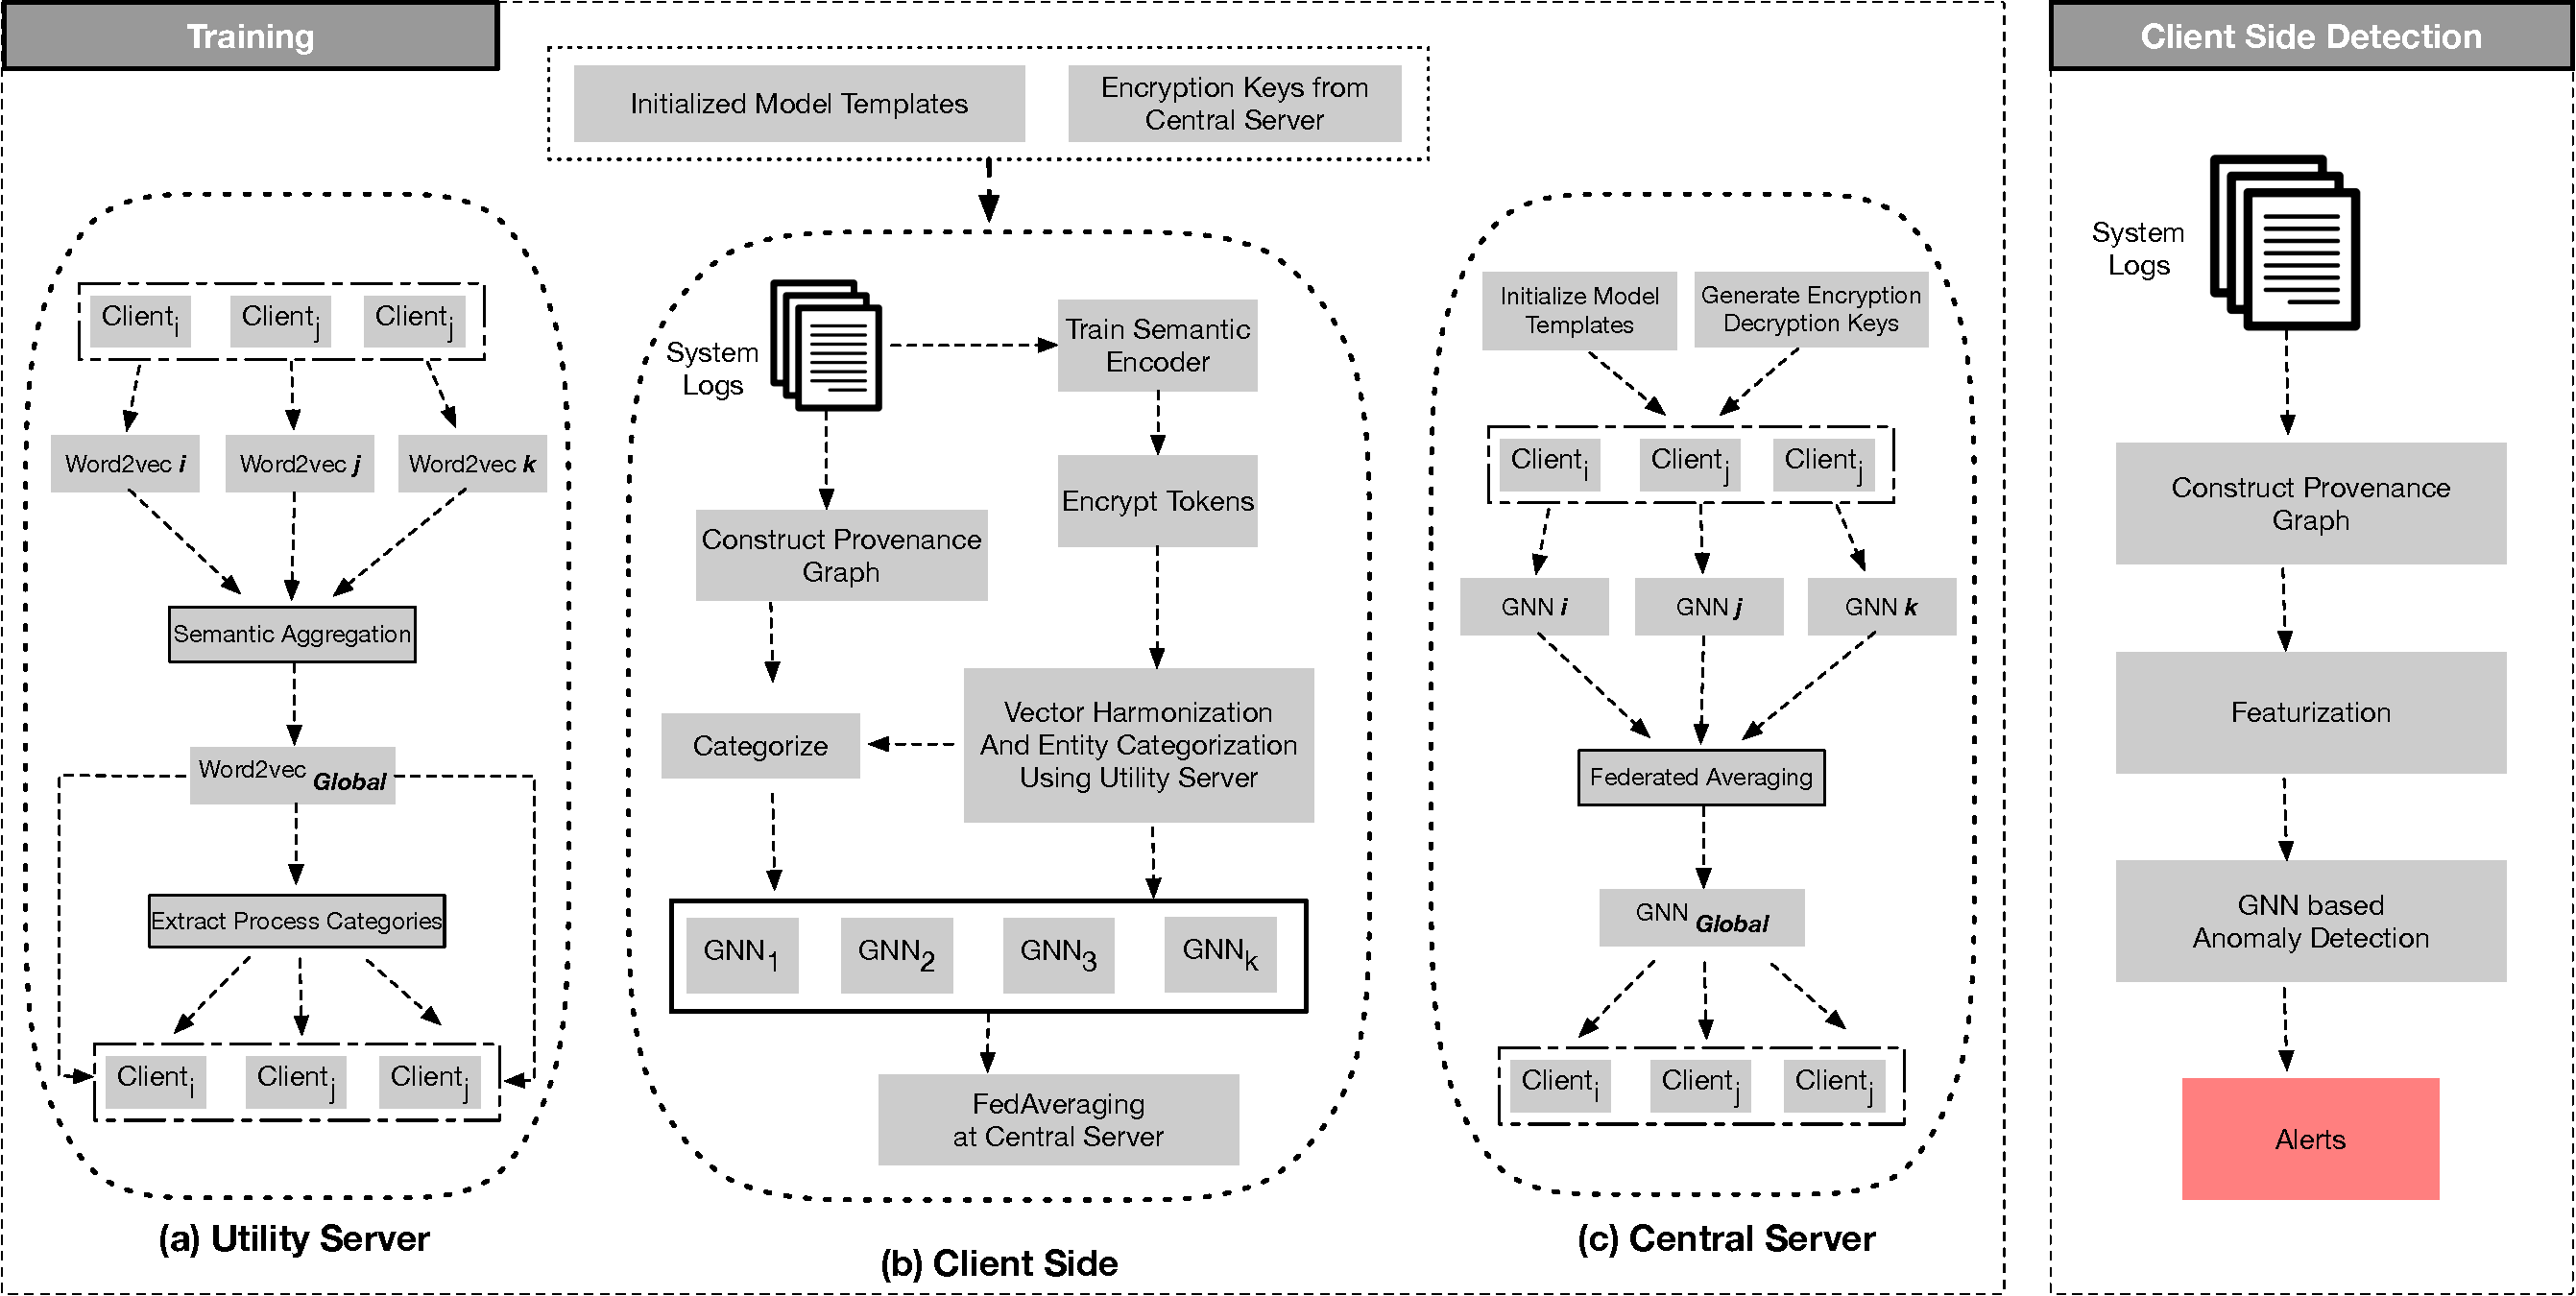
\includegraphics[width=1\textwidth]{fig/archv3.pdf}
  \caption{High-level architecture of \Sys. In the training phase, our system builds local provenance graphs for each client and trains an ensemble of \gnnshort models. Prior to this, we aggregate semantic models contextually for feature encoding. The local \gnnshort models participate in federated learning to develop a global \gnnshort model, which is then utilized for anomaly detection. Notations are defined in Table~\ref{tab:keynotations}. \wajih{lets use some notations in the Client Side Detection as well. Also, please try to use consistent terminologies in the boxes. Also connect Client 1 Client 2 arrows with Word2vec 1 and Word2vec 2. Same goves for GNN 1 and GNN2. }}
  \vspace{-3ex}
  \label{fig:arch}
\end{figure*}


\subsection{Overview}
\wajih{Make sure that subsection titles/headings match in the following paragraph. }
\Sys comprises five key modules, starting with the \textit{Provenance Graph Constructor} module (Section~\ref{sub:provconstruct}) on each client machine, which transforms logs into a provenance graph. The \textit{Semantic Featurization \& Harmonization} module (Section~\ref{semanfeat}) trains word2vec models to encode semantic attributes and consolidates individual client models into a cohesive global model using a trusted utility server and encryption techniques. The \textit{Process Entity Categorization Module} (Section~\ref{sys:catg}) standardizes system entities across clients, ensuring uniformity in GNN model training. The \textit{Federated Provenance Graph Learning Module} (Section~\ref{sys:fpgl}) then trains GNN models on each client machine using harmonized semantic features, with the models aggregated on a central server through federated averaging. Finally, the \textit{Anomaly Detection Module} (Section~\ref{sys:anomaly_detection}) applies the unified global models for anomaly detection on each client machine. Figure~\ref{fig:arch} illustrates the overall architecture of \Sys.

\subsection{Problem Statement}
\wajih{double check this subsection as I added this.}

\Sys aims to detect anomalous nodes in client-specific provenance graphs \( \{PGClient_{1}, PGClient_{2}, \ldots, PGClient_{N}\} \), which are constructed from system logs on a set of decentralized clients \( \mathcal{C} \). These anomalies represent deviations from benign behavior and are indicative of potential security threats.

To achieve this, \Sys employs a novel adaptation of Federated Learning (FL) to collaboratively train a set of global GNN models \( {GNN}_{\text{global}} = \{GNN_1, GNN_2, \ldots, GNN_{K_{cat}}\} \) without requiring raw log data to leave client machines. Each client locally optimizes its model by minimizing a loss function \( \mathcal{L}_i(w) \) and shares only model updates \( \Delta w_i \) with the central server. The global model is updated iteratively through aggregation:
\[
w = \frac{1}{N} \sum_{i=1}^{N} \Delta w_i,
\]
where \( N \) represents the total number of clients. This decentralized approach preserves privacy while enabling the detection of threats across diverse and distributed system logs. The key notations for our system are summarized in Table~\ref{tab:keynotations}.

\begin{table}[!t]
    \centering
    \scriptsize
    \caption{Key notations used in \Sys. \wajih{ Define  \( \Delta w_i \),   \( X_v \) }, \( v_k' \) }
    \label{tab:keynotations}
    \begin{tabular}{|p{3cm}|p{5cm}|}
    \hline
    \textbf{Notation} & \textbf{Definition} \\ \hline
    \( N \) & Total number of clients in federated learning. \\ \hline
    \( K_{cat} \) & Number of categories for process entities. \\ \hline
    \( \mathcal{C} = \{C_1, C_2, \ldots, C_N\} \) & Set of all client machines. \\ \hline
  
    \( PGClient_{i} = (\mathcal{V}_i, \mathcal{E}_i) \) & Provenance graph for client \( i \), with nodes \( \mathcal{V}_i \) and edges \( \mathcal{E}_i \). \\ \hline
    \( {GNN}_{\text{global}} = \{GNN_1, \ldots, GNN_{K_{cat}}\} \) & Set of global GNN models, one per category. \\ \hline
    \( w_j^{(r)} \) & Weights of global GNN for category \( j \) after round \( r \). \\ \hline
    \( \mathcal{P}_{\text{global}} \) & Global set of unique process entities. \\ \hline
    \( \psi(p) \) & Categorization map assigning process \( p \) to category \( \mathcal{C}_j \). \\ \hline
    \( y_v \) & True label of node \( v \). \\ \hline
    \( \hat{y}_v^j \) & Predicted label of node \( v \) by submodel \( j \). \\ \hline
    \( M_{\text{w2v-harm}} \) & Harmonized \wordvec model that converts contextual attributes into vector space. \\ \hline
    \( \mathcal{L}^{(r)} \) & Loss function value after round \( r \). \\ \hline
    \end{tabular}
  \end{table}

\subsection{Provenance Graph Constructor}
\label{sub:provconstruct}

\Sys utilizes \logs to construct a system provenance graph. It operates on each client machine, using their local system logs to build the graph. Major operating systems, including Linux and Windows, come equipped with built-in mechanisms for log collection -- specifically, the Linux Audit system~\cite{linuxaudit} and Windows Event Tracing~\cite{windowsaudit}. These logs provide detailed insights into the interactions among various system entities, capturing activities, such as process executions, file operations, and network connections. Using this data, \Sys forms a graph where nodes represent system entities including processes, files, and sockets. The edges of this graph denote events, identified by syscalls, that occur between these entities. Moreover, \Sys enhances each node with comprehensive attributes, including process names, command lines, file names, and network IP addresses. As demonstrated by prior works~\cite{flash2024,cheng2023kairos}, these contextual attributes enable the model to develop a robust understanding of system behavior. Figure~\ref{provexp} shows an example graph where \textit{Explorer.exe} executes processes like \textit{Notepad.exe} and \textit{Firefox.exe}, which then interact with file and socket nodes.

\begin{figure}[t!]
  \centering
  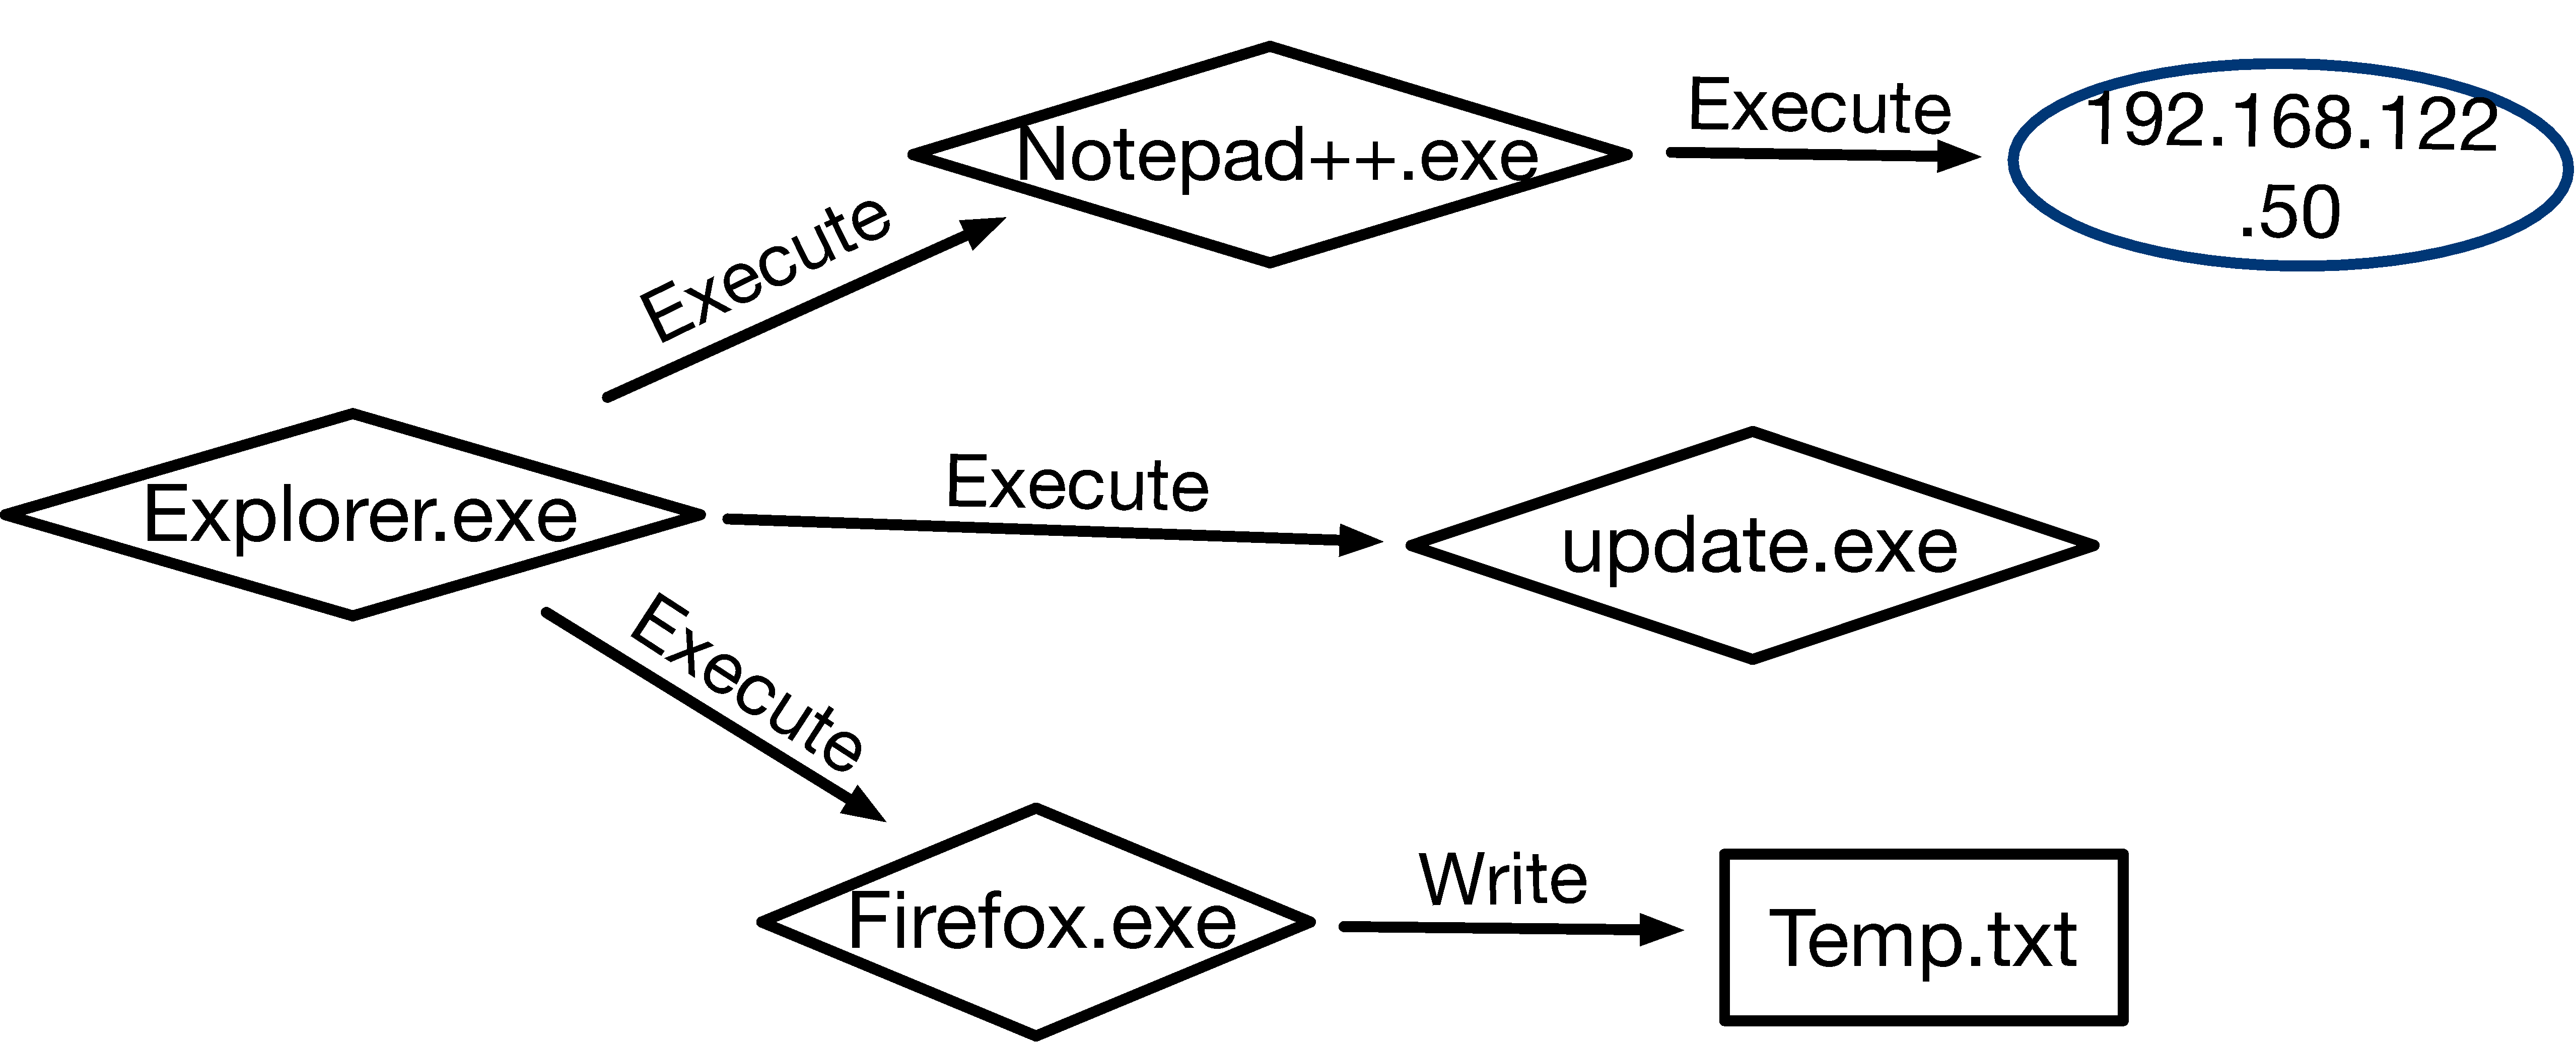
\includegraphics[width=0.4\textwidth]{fig/provexp.pdf}
  \caption{Data provenance graph example.}
  \label{provexp}
  \vspace{-3ex}
\end{figure}


\subsection{\wordvec Model Generation}
\label{sub:word2vec:model}

\wajih{this is a new subsection. If you can think of better title then use that title for this subsection. }
\wajih{use key notations if possible below.}
After provenance graph are generated on each client, the node attributes of these provenance graphs' are converted into feature vectors for the graph learning phase. Existing systems, such as \flash~\cite{flash2024}, have demonstrated the effectiveness of utilizing semantic attributes of nodes to enhance detection performance. System logs are rich in attributes related to various entities, including process names and file paths. These attributes must first be converted into vector space to serve as node features for our GNN model. For this encoding, we employ the \wordvec model.

\wajih{use key notations if possible below.}

\wajih{what is "subgraph" below. It is not clear how you generate node subgraph.}

The \wordvec model processes different attributes for each type of node: for process type nodes, it considers the process name and command line arguments; for file nodes, the file path; for socket nodes, the network IP address and port; and for module nodes, the module name. We transform the subgraph for each node into a document by combining its semantic attributes with the types of causal events, such as system calls, involving its neighbors. These documents are then transformed into fixed-length vectors using a \wordvec model trained on benign system logs. This approach effectively captures the semantic relationships between terms, producing dense embeddings that enhance the subsequent learning of graph representations.


\subsection{Privacy-preserving \wordvec Model Harmonization}
\label{sub:model:harmonization}

\PP{Addressing Token Variability Across Clients} Each client independently trains a \wordvec model using their local logs for feature encoding. However, before these models can be utilized to encode text attributes effectively, it is essential to contextually merge individual client \wordvec models into a unified model \( M_{\text{w2v-harm}} \) for use across all clients. This unification is crucial; without it, each client would produce a different encoding, \(v_a^i\), for identical inputs, where \(i\) denotes the client. The variability in feature vectors, \(\{v_a^1, v_a^2, \ldots, v_a^N\}\), for the same attribute \(a\) across \(N\) clients, would compromise the consistency of client-based \gnnshort models. To ensure uniformity, the feature vectors for overlapping attributes must be averaged across clients. Such averaging ensures consistency in the feature representation, enhancing the effectiveness of the downstream federated averaging technique by maintaining uniformity in the input space for the \gnnshort models across all clients.

Our system harmonizes only the tokens that overlap in the \wordvec models across clients. Tokens that do not overlap are not averaged and remain unchanged. While clients share common activities due to standard system-level routines, some variations and patterns are unique to each client. Non-overlapping tokens preserve these unique patterns; however, they contribute to additional heterogeneity, which cannot be eliminated through harmonization. If these unique patterns are not accurately learned, they can lead to high false alarm rates. To capture these distinct local variations between clients, we have developed a novel ensemble GNN learning framework, detailed in Section~\ref{sys:fpgl}, where each submodel specializes in distinct system patterns across clients, enhancing model precision as shown in Section~\ref{sec:eval}.

\PP{Overlap Statistics Across Clients} Our experiments with the \optc dataset revealed that, on average, different hosts can have up to 75\% overlap in process names, 41\% in files, and 60\% in network flows. This finding aligns with related work \cite{flash2024}, which shows that many system-level processes and files are common across different systems. In a centralized \pids, these attributes are learned by a single semantic model, mapping them to the same embedding space. In contrast, a federated setting, where each client trains its own model, can introduce model bias into the token embeddings, complicating the convergence for downstream GNN models using these vectors. To address this, it is essential to harmonize overlapping tokens to provide the model with a unified understanding of the semantic information present in system logs.

\wajih{The below paragraph looks very out of place. You need to connect it with the previous paragraph (the transition is missing) or move the whole paragraph somewhere else with correct transition.}

The \wordvec model functions as a key-value store, with vocabulary tokens as keys, \(k\), and their corresponding vector representations as values, \(v_k\). To combine these models, we calculate the average vector of overlapping tokens from all client machines, creating a central model. The representation for averaging vectors of a token \(k\) across \(N\) clients is given by \(\bar{v}_k = \frac{1}{N}\sum_{i=1}^{N} v_{k,i}\) where \(\bar{v}_k\) is the averaged vector for token \(k\), and \(v_{k,i}\) is the vector representation of token \(k\) from the \(i\)-th client model.


\PP{Harmonization with Encryption} However, transferring tokens -- containing sensitive data like process names, file names, and IP addresses -- to a central server could breach user privacy. To mitigate this, we employ a trusted utility server. Initially, the central server uses Fernet symmetric key encryption~\cite{ismail2020fernet,bokhari2016review} to generate an encryption key, which is distributed to clients. Clients then encrypt their \wordvec model tokens using the encryption key: \( E(v_{k}) = v_{k}^{'} \) and send them to the utility server. This server merges the encrypted models and dispatches the unified semantic vectors back to the respective clients, who decrypt them back: \( D(v_{k}^{'}) = v_{k} \). This procedure ensures that neither the central server nor the utility server can access the actual token information, assuming no collusion between the two servers. The process is detailed in Algorithm~\ref{alg:secure_integration_averaging_word2vec}.

\begin{algorithm}[!t]
    \scriptsize
    \DontPrintSemicolon
    \SetKwInOut{Input}{Inputs}
    \SetKwInOut{Output}{Output}
    \Input{Client Word2Vec models $\{Word2vec_1, Word2vec_2, \ldots, Word2vec_N\}$.}
    \Output{Harmonized Word2Vec model $M_{\text{w2v-harm}}$ sent to clients.}
    \BlankLine
    \tcc{Central server distribute symmetric encryption keys to each client.}
    \ForEach{client $C_i$}{
  
      Send $key$ to $C_i$\\
    }
    \tcc{Clients encrypt their model tokens.}
    \ForEach{client model $word2vec_i$}{
      $Word2vec_i \leftarrow$ EncryptModelTokens($Word2vec_i$, $E$) \tcc*{Encrypt tokens using $E$.}
      Send $Wor2vec_i$ to Utility Server\\
    }
    \tcc{Utility server merges encrypted models.}
    $TokenVectors \leftarrow$ InitializeEmptyDictionary()\\
    $TokenCounts \leftarrow$ InitializeEmptyDictionary()\\
    \ForEach{encrypted model $Word2vec_i$}{
      \ForEach{token $t$ in $Word2vec_i$}{
        $Vector \leftarrow Word2vec_i[t]$\\
        \eIf{$TokenVectors$.HasKey($t$)}{
          $TokenVectors[t] \leftarrow TokenVectors[t] + Vector$\\
          $TokenCounts[t] \leftarrow TokenCounts[t] + 1$\\
        }{
          $TokenVectors[t] \leftarrow Vector$\\
          $TokenCounts[t] \leftarrow 1$\\
        }
      }
    }
    \tcc{Average the vectors for overlapping tokens.}
    \ForEach{token $t$ in $TokenVectors$.Keys()}{
      $TokenVectors[t] \leftarrow TokenVectors[t] / TokenCounts[t]$\\
    }
    $M_{\text{w2v-harm}} \leftarrow$ NewModel($TokenVectors$, $EncryptedTokens$) \tcc*{Constructing a new harmonized model.}
    \ForEach{client $C_i$}{
      Send $M_{\text{w2v-harm}}$ to $C_i$\\
    }
    \BlankLine
    \Return{Harmonized model $M_{\text{w2v-harm}}$ has been dispatched to all clients.}\\
    \BlankLine
    \caption{Privacy-preserving \wordvec Model Harmonization.}
    \label{alg:secure_integration_averaging_word2vec}
  \end{algorithm}

\subsection{Process Entity Categorization}
\label{sys:catg}

During our initial experiments (Table~\ref{categorized_gnn}), we found that a single \gnnshort global model cannot achieve good detection performance in an FL setting due to the diverse and heterogeneous distributions of clients data. The disparity in data distributions among \( N \) clients poses a significant challenge in effectively training a unified model that can generalize well across all clients, since the global model struggles to capture the unique characteristics and patterns inherent in each client's data.

% \wajih{use key notations below if possible.}
To address this limitation, we developed a comprehensive framework that organizes process entities across different clients into distinct groups. Each category is modeled by a dedicated submodel, enabling it to focus on the unique distribution and intricate patterns of its assigned category and thereby enhance overall detection performance.

% \wajih{please refer to algorithm in the whole paragraph. Divide the following paragraph into three steps using latex enumerate macro.}
As shown in \Fix{Algorithm~\ref{alg:categories}}, the framework leverages a central utility server to orchestrate the categorization of process entities. Specifically, it proceeds in three main steps:
\begin{enumerate}
    \item \textbf{Collection of Encrypted Process Names.} Each client \(C_i \in \mathcal{C}\) transmits an encrypted list of its process names to the utility server. The server merges these into a global list of unique process entities, denoted by \( \mathcal{P}_{\text{global}} \).

    \item \textbf{Random Categorization.} The utility server applies the categorization map \( \psi(p) \) to randomly partition all process names in \( \mathcal{P}_{\text{global}} \) into \( K_{cat} \) categories. Although the partitioning is random, it is performed only once at the global level, ensuring that any process name \( p \) is consistently mapped to the same category \( j \) across all clients, i.e., \( \psi(p) = j \).

    \item \textbf{Distribution of Categories.} Finally, the resulting category assignments are disseminated back to each client, guaranteeing a unified and consistent mapping of processes into categories across the federated network.
\end{enumerate}

\begin{algorithm}[!t]
    \scriptsize
    \DontPrintSemicolon
    \SetKwInOut{Input}{Inputs}
    \SetKwInOut{Output}{Output}
    \caption{Categorizing processes into \(\,K_{cat}\) categories.}
    \label{alg:categorization_process}
  
    \Input{
      Number of clients \(N\); Number of categories \(K_{cat}\); Client datasets \(\mathcal{C}\)
    }
    \Output{
      Category assignment function \(\psi\)
    }
  
    \BlankLine
    \tcc{Step 1: Initialization of utility server and global process list.}
    \(\mathcal{P}_{\text{global}} \leftarrow \emptyset\) \\
    \ForEach{client \(C_i \in \mathcal{C}\)}{
        Transmit encrypted process list to utility server \\
        \(\mathcal{P}_{\text{global}} \leftarrow \mathcal{P}_{\text{global}} \cup \text{Encrypt}(C_i)\)
    }
  
    \BlankLine
    \tcc{Step 2: Categorization of processes into \(K_{cat}\) categories.}
    \For{\(p \in \mathcal{P}_{\text{global}}\)}{
        \(\psi(p) \leftarrow \text{RandomCategory}(K_{cat})\)
    }
  
    \BlankLine
    \tcc{Step 3: Distribute global category assignments to clients.}
    \ForEach{client \(C_i \in \mathcal{C}\)}{
        Send categorization \(\psi\) to \(C_i\)
    }
  
    \BlankLine
    \Return \(\psi\)
    \label{alg:categories}
  \end{algorithm}

% Once the categories are established, each client employs the categorized process sets to build provenance subgraphs \( PGClient_{i} \). The neighborhood hop length of these subgraphs is aligned with the number of graph convolution layers in \( {GNN}_{\text{global}} \), ensuring the model has complete neighborhood information for each node. In our experiments, we fix this hop length to two, which past studies~\cite{wang2022threatrace,flash2024} have shown to offer an optimal trade-off between efficiency and accuracy. These subgraphs provide training data for an ensemble of \({GNN}_{\text{global}}\) models in a federated manner. Each submodel specializes in learning the patterns of its assigned category and participates in federated averaging. This ensures a balanced segmentation of data across clients and maintains consistency in the training datasets for each submodel before federated averaging.

% \wajih{move this example at the of this subsection. Make sure that transitions among all the paragraphs is smooth.}
To illustrate this process, consider two clients: \emph{A} and \emph{B}:
\begin{itemize}[itemsep=0.1em, parsep=0em, topsep=0em, leftmargin=*]
    \item \emph{A} has a set of processes \{\texttt{chrome}, \texttt{ssh}, \texttt{mysql}\}.
    \item \emph{B} has a set of processes \{\texttt{chrome}, \texttt{firefox}, \texttt{ssh}, \texttt{mysql}\}.
\end{itemize}
Both clients send encrypted lists of these process names to the utility server, which combines them into a single global list of unique names \{\texttt{chrome}, \texttt{ssh}, \texttt{mysql}, \texttt{firefox}\}. The server then applies \( \psi \) to randomly assign each name to one of the \( K_{cat} \) categories. For example, \( \psi(\texttt{chrome}) \) and \( \psi(\texttt{mysql}) \) may map to category~1, while \( \psi(\texttt{ssh}) \) and \( \psi(\texttt{firefox}) \) map to category~2.

This assignment is transmitted back to both clients, ensuring that \texttt{chrome} and \texttt{mysql} are consistently grouped under category~1, and \texttt{ssh} and \texttt{firefox} under category~2. As a result, each category gathers similar processes across all clients, even though the initial split is random. By dividing the overall task into sub-tasks (submodels) and distributing them to different subsets of processes, the influence of clients with larger datasets is shared among multiple models. This approach reduces the risk of any single client dominating the federated training process and facilitates more balanced contributions from all participants, ultimately improving the robustness and performance of the system.

\subsection{FL using Categorized Process Entities}
\label{sys:fpgl}

\begin{algorithm}[!t]
    \scriptsize
    \DontPrintSemicolon
    \SetKwInOut{Input}{Inputs}
    \SetKwInOut{Output}{Output}
    \caption{Training and federated aggregation of category-specific submodels.}
    \label{alg:training_submodel}
  
    \Input{
      Global process list \(\mathcal{P}_{\text{global}}\), \\
      Category assignment function \(\psi\), \\
      Number of categories \(K_{cat}\), \\
      Client datasets \(\mathcal{C}\)
    }
    \Output{
      Trained global GNN models \(\text{GNN}_{\text{global}}\)
    }
  
    \BlankLine
    \tcc{Step 1: Local training of submodels for each category.}
    \ForEach{client \(C_i \in \mathcal{C}\)}{
        \ForEach{\(p \in C_i\)}{
            \(j \leftarrow \psi(p)\) \\
            Train GNN submodel on processes in category \(j\) from client \(C_i\)
        }
    }
  
    \BlankLine
    \tcc{Step 2: Aggregation and federated averaging of submodels.}
    \ForEach{category \(j \in \{1, \ldots, K_{cat}\}\)}{
        \(w_j^{(0)} \leftarrow \text{InitializeRandomWeights}()\) \\
        \ForEach{client \(C_i \in \mathcal{C}\)}{
            \(w_j^{(i)} \leftarrow \text{ExtractWeights}(C_i, j)\)
        }
        \(\displaystyle w_j^{(r)} \leftarrow \text{FederatedAveraging}\bigl(\{w_j^{(i)}\}\bigr)\)
    }
  
    \BlankLine
    \Return \(\displaystyle \text{GNN}_{\text{global}} \leftarrow \{\,w_1^{(r)},\, w_2^{(r)},\, \ldots,\, w_{K_{cat}}^{(r)}\}\)
    \label{alg:submodel}
  \end{algorithm}
  


% \wajih{First paragraph should connect this subsection with the previous subsection. Say something like "Once the blah blah is generated in the previous module (Section{}), we can use these blah blah for blah blah. However, blah blah is not possible without blah blah.}

%\wajih{Is process entitiy categorization related to Categorized Provnenace subgraph? it is not clear at all. Please do not use words without connecting them with the broader context.}

% \wajih{move this paragraph to discussion section why we combine FL with GNN.}
% APTs involve multiple causally linked attack steps across various system entities, highlighting the need to capture and model the interactions among these entities for effective detection. Analyzing each system event in isolation does not allow us to capture these interactions properly, as observed in existing log-level systems~\cite{deeplog2017,liu2019log2vec,xia2019loggan}; hence, provenance graphs, \( PGClient_{i} \), are being used to effectively model the interaction of system entities. Moreover, graph representation learning is used to learn the patterns present in these graphs, as shown in related works~\cite{flash2024,cheng2023kairos,jia2023magic}. We integrate federated learning with graph representation learning to bring privacy and decentralization to intrusion detection while maintaining the strong detection performance offered by the provenance graph learning technique.

% \wajih{Refer to the Algorithm throught the paragraph. use steps just like you have in the algorithm. Maybe break this paragraph into multiple paragraph otherwise this subsection will look very small. }
% Our approach includes a central server responsible for initializing the global GNN models, \({GNN}_{\text{global}}\), with random weights, \( w_j^{(0)} \), which are then sent to all clients in \( \mathcal{C} \). These clients use their local process subgraphs, \( PGClient_{i} \), and semantic feature vectors to train the GNN models in an unsupervised way, following a training method similar to \flash. The objective of the GNN model is to classify each node \( v \) into its corresponding type, yielding predictions \(\hat{y}_v^j\). The server then applies the federated averaging algorithm to merge the GNN models into a set of global models, \({GNN}_{\text{global}}\), based on the process entity categories on which they were trained. This ensures that models with similar distributions are combined together to address the data heterogeneity problem. Specifically, the server aggregates parameters from \( N \) client models to update each global submodel as \(\bar{w} = \frac{1}{N} \sum_{i=1}^{N} w_i\). Algorithm~\ref{alg:training_submodel} explains this process in detail.

% The federated averaging process is repeated for a set number of rounds \( R \), and concludes when there is no further reduction in the training loss, \(\mathcal{L}^{(r)}\). 
Once the categorized bins of processes have been generated, we train specialized GNN models for each bin. Each \({GNN}_{\text{global}}\) submodel focuses on a standardized subset of processes across clients, identified through entity categorization. This approach effectively captures distinct patterns and structures while reducing data heterogeneity. Our method proceeds in three main steps, as detailed in Algorithm~\ref{alg:training_submodel}.

\textbf{Step 1: Initialization.} As in Step~1 of Algorithm~\ref{alg:training_submodel}, the central server initializes the global GNN models, \({GNN}_{\text{global}}\), with random weights \( w_j^{(0)} \). The server then transmits these initial weights \( w_j^{(0)} \) to all clients in \(\mathcal{C}\).

\textbf{Step 2: Local Model Training.} Each client \( C_i \) organizes its local processes into bins based on the assigned categories, \(\psi(p)\) which it gets using the methodology detailed in section~\ref{sys:catg}. From each category bin, the client constructs a \emph{provenance subgraph} capturing the local relationships of processes within that category. The neighborhood hop length of these subgraphs matches the number of graph convolution layers in \({GNN}_{\text{global}}\), ensuring the model has sufficient neighborhood information for each node. Each client then leverages these categorized subgraphs, along with semantic feature vectors, to train the GNN models in an unsupervised manner. Similar to the approach in \flash, the objective of each GNN submodel is to classify every node \(v\) into its corresponding type, yielding predictions \(\hat{y}_v^j\). This localized, category-focused training ensures that each submodel effectively captures the unique structures and distributions within each category for the client’s data.

\textbf{Step 3: Federated Averaging and Category-Based Aggregation.} As in Step~2 of Algorithm~\ref{alg:training_submodel}, the server collects the updated parameters from all \( N \) clients for each category-specific submodel. It then applies the federated averaging algorithm to merge these parameters, computing
\(
\bar{w} \;=\; \frac{1}{N} \sum_{i=1}^{N} w_i
\) for each category’s global submodel. Because every submodel is trained on processes belonging to the same category across all clients, the data distributions within each submodel are more homogeneous, effectively addressing data heterogeneity. This category-based aggregation integrates knowledge gained from multiple clients, leading to robust, specialized global models.

The federated averaging process (Step~3 of Algorithm~\ref{alg:training_submodel}) is repeated for \( R \) rounds, concluding once there is no further reduction in the training loss \(\mathcal{L}^{(r)}\). The resulting ensemble of global submodels, each attuned to a distinct process category, provides a comprehensive solution that balances the diverse data distributions across clients while preserving privacy.

\subsection{GNN-based Anomaly Detection}
\label{sys:anomaly_detection}

\Sys employs a node level detection methodology focusing on identifying irregular nodes through the comparison of their expected and observed types. This approach is grounded in a detailed analysis of both the surrounding structures and inherent properties of the nodes, to define normal pattern baselines for various node types. Typically, entities with malicious intentions display neighborhood structures and characteristics deviating from these established norms as shown in previous work~\cite{flash2024,cheng2023kairos,yangprographer}. In operational phases, the detection of anomalies that diverge from the pre-established node distribution patterns often results in their misclassification. The emergence of nodes misclassified in the system's output is indicative of potential security issues.

\Sys performs threat detection in a decentralized manner on clients' provenance graphs (\( \{PGClient_{1}, PGClient_{2}, \ldots, \\ PGClient_{N}\} \)) in an organization. For a given provenance graph \(PGClient_{i}\), \Sys uses the global \gnnshort models \(\{GNN_1, \\ GNN_2, \ldots, GNN_{K_{cat}}\}\) trained using federated learning. Each submodel performs inference on the client's full provenance graph, utilizing the nodes' features \(X_v\) and the graph's adjacency matrix \(A\) to predict each node \(v\)'s label \(\hat{y}_v^j\). Let us define a misclassification indicator \(\mathcal{M}(v, j)\) as
\[
\mathcal{M}(v, j) \;=\;
\begin{cases}
1, & \text{if } \hat{y}_v^j \neq y_v,\\
0, & \text{otherwise}.
\end{cases}
\]
Accordingly, a node \(v\) is identified as an anomaly if it is misclassified by \emph{all} submodels, i.e.,
\[
\mathcal{A}(v) \;=\;
\begin{cases}
1, & \text{if } \sum_{j=1}^{K_{cat}} \mathcal{M}(v, j) \;=\; K_{cat},\\
0, & \text{otherwise}.
\end{cases}
\]
This indicates that none of the submodels recognize the neighborhood structure or features displayed by \(v\), prompting its classification as an anomaly.


To regulate the frequency of alerts, we define a threshold \(T\) similar to \flash. This parameter sets a threshold on the likelihood of a classification being considered valid, with a higher value of \(T\) implying stronger confidence and increasing the probability of identifying anomalies.

% \section{Implementation}
\label{s:impl}

 \section{Evaluation}
 \label{sec:eval}

%  \wajih{Be consistent with datasets in each research question. Sometimes you use OpTC and sometimes you use E3 and you don't even explain why you excluded the other datasets. Rule of thumb is use all the datasets for the experiments unless you have reason or justification why you excluded certain datasets.}

 %\mati{Evaluation section has some writing inconsistencies. I will make a pass over it later today to fix it.}

%  \wajih{the word DISTDET is not consistent in the paper.}

 %\wajih{Use macros for common words in this whole section.}

 %\wajih{Be consistent with the terminology that you used in the abstract/intro.}

 %\wajih{Captions need to be lowercase}



%We evaluate \Sys using the open-source datasets \darpa E3 and \optc, which comprise system audit logs that simulate enterprise environments. These logs are collected from both Windows and Linux operating systems.



%\wajih{We also need to handle as ORTHRUS in the related work or evaluation section. I would love to hear creative way we can handle that.}

%\wajih{Handle this comment in the evaluation section: "I'm quite concerned about the evaluation results in Table 2. It doesn't look right to me that the number of malicious nodes in DARPA TC datasets can be sometimes around 20\%!"}

\wajih{ We claim that the categorization-based ensemble improves convergence. But there is no empirical convergence analysis in the evaluation section e.g., training loss curves or number of FL rounds, etc. }

\wajih{Add in the evaluation section how many clients we have in each dataset. "I can't find the number of FL clients in your text" }

Our evaluation experiments are conducted on a machine running Ubuntu 18.04.6 LTS, equipped with a 10-core Intel CPU, NVIDIA RTX 2080 GPU, and 120 GB of memory. In our experiments, we set the federated learning rounds and the number of categorized \gnnshort to 10 per host. Each model is trained for 20 epochs per round. We use regularization and dropout layers in our models to avoid overfitting. To evaluate \Sys, we address the following research questions: \wajih{I have moved things around so align the RQs with that.}

%\wajih{RQ6 is not in this section. so please remove it. }

%\wajih{Add section references like I added for RQ1}

% \Fix{There are eight subsection in the evaluation while we have six research question. Make them consistent. This can confuse reader. Also, if you moved something to Appendix, refer them below. }

% \wajih{These are just too many research question. You need to combine similar RQs into one. If you think something is an ablation study then move it to the ablation study section. }
\begin{itemize}[leftmargin=*,itemsep=0.1em, parsep=0em, topsep=0em]
  \item \textbf{RQ1.} How does \Sys compare to existing systems in terms of detection performance? (Section~\ref{sub:detect:perf})
  \item \textbf{RQ2.} How effective is the Word2vec harmonization scheme for handling feature heterogeneity? (Section~\ref{sub:word2vec:harmonization:efficacy})
  \item \textbf{RQ3.} How effective is the categorization-based \gnnshort ensemble for handling data heterogeneity? (Section~\ref{sub:categorized:learning:efficacy})
  \item \textbf{RQ4.} How does \Sys compare to existing FL solutions in addressing data heterogeneity and non-IID challenges? (Section~\ref{sec:fedalternatives})
  \item \textbf{RQ5.} How scalable is \Sys in an enterprise-level setting with multiple host machines? (Section~\ref{cost_metric})
  % \item \textbf{RQ6.} How robust is \Sys against adversarial mimicry attacks?
  \item \textbf{RQ6.} What is the resource consumption of various components of \Sys and its end-to-end processing time on a client machine? (Appendix~\ref{sec:resource_consumption})
  \item \textbf{RQ7.} What does the ablation study reveal about \Sys's scalability and effectiveness across key factors like \gnnshort submodels, averaging rounds, federated averaging rounds, etc.? (Appendix~\ref{app:ablation})
  
  \end{itemize}  


\PP{Implementation} \Sys is developed in Python with around 5500 lines of code. It leverages the PyTorch and Torch Geometric libraries to implement the federated provenance graph learning framework. The graph learning framework uses the GraphSAGE~\cite{hamilton2017inductive} family of \gnnshort. Our architecture consists of two graph convolution layers with a Tanh activation function in between. The last layer uses a softmax function to output class probabilities for the nodes. For implementing the \wordvec model, we employ the Gensim library. Secure communication between clients and the utility server is ensured through Python's Cryptography module. The federated averaging, semantic vector harmonization, and entity categorization modules are implemented as individual Python functions on the central and utility servers.

% \PP{Datasets} We have utilized the \darpa E3~\cite{error3}, E5~\cite{bug5}, and \optc~\cite{darpaoptc} datasets for our evaluation. The E3 and E5 datasets consist of several adversarial engagements that simulate real-world APTs on enterprise networks. In these exercises, the red team aims to exploit vulnerabilities in the enterprise's services while hiding their attacks behind benign system activities. The logs captured from these exercises are documented under various scenario names, including Cadets, Trace, Theia and ClearScope. The \optc dataset, another open-source resource from \darpa, encompasses a comprehensive collection of audit logs from an enterprise environment with 1,000 hosts. This dataset includes six days of benign system logs, serving as training data for our system to learn normal behavior patterns. Subsequently, attack logs span three days of system activities, featuring red team tactics such as initial compromises, privilege escalations, malicious software installations, and data exfiltration. Each of these datasets is accompanied by ground truth documents that facilitate the distinction between benign and malicious events. For our evaluation, we employ attack labels from existing systems, such as \threatrace, \kairos and \flash for our evaluation. We evaluate our system using the same subset of datasets as existing open-source systems such as \kairos and \flash, and we utilize the attack node labels provided by them to ensure fairness.

\PP{Datasets} We have utilized the \darpa E3~\cite{error3}, E5~\cite{bug5}, and \optc~\cite{darpaoptc} datasets for our evaluation. These datasets contain real-world APT attacks observed in enterprise networks. The attack traces they include are stealthy, span several days, and mirror the characteristics of actual APTs. Consequently, achieving strong detection accuracy on these datasets indicates that our system can deliver comparable performance in real-world deployments. Furthermore, these datasets incorporate logs of various sizes from Linux, FreeBSD, Android, and Windows operating systems. Our system’s robust detection accuracy across all datasets demonstrates its effective generalization to heterogeneous platforms with differing log sizes, reaching performance levels on par with state-of-the-art centralized \pids. Notably, the datasets capture APT attacks of varying stealthiness, with the proportion of malicious nodes ranging from 0.05\% in \optc to 2\% in E3, and approximately 19\% in E5. The low infiltration rate in \optc underscores the system’s capacity for detecting highly stealthy adversaries, whereas the more widespread attacks in E5 highlight the resilience of our approach when confronted with a higher density of malicious nodes. Collectively, these datasets serve as a strong benchmark to evaluate the scalability and adaptability of our system. Each \darpa dataset is accompanied by ground truth documents that aid in distinguishing benign events from malicious ones. For this evaluation, we employ attack labels from existing systems such as \threatrace, \kairos, and \flash. Further details regarding the datasets appear in Appendix~\ref{sec:dataset:description}. ATLASv2~\cite{riddle2023atlasv2} is another recent dataset containing APT attack traces, but we did not evaluate it because it only includes data from two hosts, making it unrepresentative of a typical federated learning scenario.




\PP{Detectors for comparison} To benchmark our system, we conduct comparisons against existing state-of-the-art \pids. \threatrace~\cite{wang2022threatrace}, a node-level system, employs graph representation learning to identify anomalous nodes within a provenance graph. MAGIC~\cite{jia2023magic} is another recent \pids which uses masked graph representation learning to detect system threats. \flash~\cite{flash2024} is another notable node-level system, which utilizes semantic feature vectors and an embedding recycling database to offer superior detection performance and efficiency. \flash detection results, as shown in Table~\ref{summary:benchmarks:large}, have been shown to surpass \threatrace. Hence, our comparison primarily focuses on \flash. Additionally, we include \kairos~\cite{cheng2023kairos} in our comparison, which utilizes temporal graph networks to capture the evolution of a system's provenance graph over time.

\PP{Excluded Detectors} We do not compare against Streamspot~\cite{streamspot} and Unicorn~\cite{han2020unicorn} as they are graph-level detectors, and recent systems like \threatrace and \flash have been shown to surpass them in detection performance. While \disdet~\cite{dong2023distdet}, Prographer~\cite{yangprographer} and Shadewatcher~\cite{shadewatcher} are notable \pids, we exclude them from our comparison because \disdet and Prographer are closed-source and a major component of Shadewatcher is proprietary, which hinders our ability to conduct a thorough comparison. It is important to note that, similar to existing works (e.g., \kairos, Shadewatcher, and Prographer), \Sys considers only three node types in provenance graphs: \emph{processes}, \emph{files}, and \emph{sockets}. However, in the E3 dataset, \flash has also been evaluated using additional node types. Therefore, we executed \flash using these three node types to report the results in Table~\ref{summary:benchmarks:large}.


\subsection{Detection Performance Against a Vanilla Privacy-Preserving PIDS}
\label{sub:detect:perf:vanilla}

\wajih{Add a line about Vanilla Privacy-Preserving PIDS and how it was created by using basic FL with Flash. and say that Besides Flash we tried other SOTA PIDS and we got similar results for Vanilla Privacy-Preserving PIDS so we only include results for Flash.}

\wajih{Add results and table for Vanilla Privacy-Preserving PIDS}

\begin{table*}[!t]
  \centering
  \scriptsize
  \caption{Comparison of \Sys against vanilla privacy-preserving PIDS as baseline.}
  \setlength{\tabcolsep}{4pt} % slightly narrower columns
  \renewcommand{\arraystretch}{1} % optional: improves vertical spacing
  \begin{tabular*}{\textwidth}{@{\extracolsep{\fill}}lcccccccccccccc}
    \toprule
    \multirow{2}{*}{\textbf{Dataset}} &
    \multicolumn{7}{c}{\textbf{Baseline}} &
    \multicolumn{7}{c}{\textbf{\Sys}} \\
    \cmidrule(lr){2-8} \cmidrule(lr){9-15}
    & Precision & Recall & F1-score & TP & FP & FN & TN
    & Precision & Recall & F1-score & TP & FP & FN & TN \\
    \midrule
    E3-CADETS       & 0.64 & 0.99 & 0.78 & 12846 & 7243 & 4 & 699725
                    & \TCP & \TCR & \TCF & \TCTP & \TCFP & \TCFN & \TCTN \\
    E3-TRACE        & 0.85 & 0.99 & 0.92 & 67357 & 11390 & 20 & 2404623
                    & \TTP & \TTR & \TTF & \TTTP & \TTFP & \TTFN & \TTTN \\
    E3-THEIA        & 0.69 & 0.99 & 0.81 & 25314 & 11337 & 38 & 3493999
                    & \TTHP & \TTHR & \TTHF & \TTHTP & \TTHFP & \TTHFN & \TTHTN \\
    OpTC            & 0.36 & 0.99 & 0.53 & 649 & 1142 & 1 & 1286213
                    & \TOP & \TOR & \TOF & \TOTP & \TOFP & \TOFN & \TOTN \\
    E5-CADETS       & 0.76 & 0.99 & 0.86 & 40098 & 12356 & 10 & 1258638
                    & \ETCP & \ETCR & \ETCF & \ETCTP & \ETCFP & \ETCFN & \ETCTN \\
    E5-THEIA        & 0.73 & 0.99 & 0.84 & 54810 & 20767 & 270 & 1250910
                    & \ETTHP & \ETTHR & \ETTHF & \ETTHTP & \ETTHFP & \ETTHFN & \ETTHTN \\
    E5-ClearScope   & 0.79 & 0.97 & 0.88 & 13670 & 3491 & 397 & 79857
                    & \ETClP & \ETClR & \ETClF & \ETClTP & \ETClFP & \ETClFN & \ETClTN \\
    \bottomrule
  \end{tabular*}
  \label{summary:benchmarks:vanilla}
\end{table*}


 \subsection{Detection Performance Against SOTA PIDS}
 \label{sub:detect:perf}

 \renewcommand{\arraystretch}{1}
\begin{table*}[!t]
  \centering
  \scriptsize
  \caption{Comparison of \Sys with SOTA PIDS. Prec.: Precision; Rec.: Recall; F1.: F1-Score. While \flash performs slightly better, \Sys offers strong privacy and scalability through decentralization. Refer to SOTA PIDS papers for their FP/FN details. The fraction in parentheses for Mirage indicates how many systems (out of the total compared) it outperforms or matches on that metric.}
  \setlength{\tabcolsep}{1pt}
  \newcolumntype{Y}{>{\centering\arraybackslash}X}
  \begin{tabularx}{\textwidth}{l*{4}{YYY}G{1.4cm}G{1.4cm}G{1.4cm}}
    \toprule
    \textbf{Dataset}
    & \multicolumn{3}{c}{\textbf{MAGIC~\cite{jia2023magic}}}
    & \multicolumn{3}{c}{\textbf{\flash~\cite{flash2024}}}
    & \multicolumn{3}{c}{\textbf{\kairos~\cite{cheng2023kairos}}}
    & \multicolumn{3}{c}{\textbf{\orthrus~\cite{jiang2025orthrus}}}
    & \multicolumn{3}{c}{\textbf{\Sys}} \\
    \cmidrule(r{2pt}){2-4} \cmidrule(r{2pt}){5-7} \cmidrule(r{2pt}){8-10} \cmidrule(r{2pt}){11-13} \cmidrule(l){14-16}
      & Prec. & Rec. & F1.
      & Prec. & Rec. & F1.
      & Prec. & Rec. & F1.
      & Prec. & Rec. & F1.
      & Prec. & Rec. & F1.   \\
    \midrule
    E3-CADETS       & 0.94 & 0.99 & 0.97 & \FCP  & \FCR  & \FCF  & \KCP  & \KCR  & \KCF  & 0.52 & 0.37 & 0.43 & \TCP~(\ccmark{3/4}) & \TCR~(\ccmark{3/4}) & \TCF~(\ccmark{3/4}) \\
    E3-TRACE        & 0.99 & 0.99 & 0.99 & \FTP  & \FTR  & \FTF  & --    & --    & --    & --    & --    & --  & \TTP~(\ycmark{0/3}) & \TTR~(\ccmark{3/3}) & \TTF~(\ycmark{0/3}) \\
    E3-THEIA        & 0.98 & 0.99 & 0.99 & \FTHP & \FTHR & \FTHF & \KTHP & \KTHR & \KTHF & 0.81 & 0.40 & 0.54 & \TTHP~(\ycmark{2/4}) & \TTHR~(\ccmark{3/4}) & \TTHF~(\ycmark{2/4}) \\
    \optc           & --   & --   & --   & \FOP  & \FOR  & \FOF  & \KOP  & \KOR  & \KOF  & --   & --   & --   & \TOP~(\ycmark{1/2}) & \TOR~(\ycmark{1/2}) & \TOF~(\ycmark{1/2}) \\
    E5-CADETS       & 0.00 & 1.00 & 0.00 & \EKCP & \EKCR & \EKCF & \EFCP & \EFCR & \EFCF & 0.17 & 0.02 & 0.03 & \ETCP~(\ycmark{2/4}) & \ETCR~(\ccmark{3/4}) & \ETCF~(\ycmark{2/4}) \\
    E5-THEIA        & 0.00 & 0.00 & 0.00 & \EKTHP & \EKTHR & \EKTHF & \EFTHP & \EFTHR & \EFTHF & 0.87 & 0.19 & 0.31 & \ETTHP~(\ccmark{4/4}) & \ETTHR~(\ccmark{3/4}) & \ETTHF~(\ccmark{4/4}) \\
    E5-ClearScope   & 0.00 & 1.00 & 0.00 & \EKClP & \EKClR & \EKClF & \EFClP & \EFClR & \EFClF & 0.33 & 0.08 & 0.13 & \ETClP~(\ccmark{4/4}) & \ETClR~(\ccmark{3/4}) & \ETClF~(\ccmark{4/4}) \\
    \bottomrule
  \end{tabularx}
  \label{summary:benchmarks:large}
\end{table*}

% \renewcommand{\arraystretch}{1}
% \begin{table*}[!t]
%   \centering
%   \scriptsize
%   \caption{Comparison of \Sys with SOTA PIDS. Prec.: Precision; Rec.: Recall; F1.: F1-Score. While \flash performs slightly better, \Sys offers strong privacy and scalability through decentralization. Refer to SOTA PIDS papers for their FP/FN details. The fraction in parentheses for Mirage indicates how many systems (out of the total compared) it outperforms or matches on that metric. \wajih{This looks SUPER bad. Could you bring back the previous one without grey }}
%   \setlength{\tabcolsep}{4pt}
%   \newcolumntype{Y}{>{\centering\arraybackslash}X}
%   \begin{tabularx}{\textwidth}{lYYYYYYY}
%     \toprule
%     \textbf{Dataset}
%     & \textbf{Ortrhurs}
%     & \textbf{MAGIC~\cite{jia2023magic}}
%     & \textbf{\flash~\cite{flash2024}}
%     & \textbf{\kairos~\cite{cheng2023kairos}}
%     & \multicolumn{3}{c}{\textbf{\Sys}} \\
%     \cmidrule(r{4pt}){2-2} \cmidrule(r{4pt}){3-3} \cmidrule(r{4pt}){4-4} \cmidrule(r{4pt}){5-5} \cmidrule(lr){6-8}
%       & {\bf Prec./Rec./F1.}
%       & {\bf Prec./Rec./F1.}
%       & {\bf Prec./Rec./F1.}
%       & {\bf Prec./Rec./F1.}
%       & \textbf{Prec.} & \textbf{Rec.} & \textbf{F1.} \\
%     \midrule
%     E3-CADETS       & 0.52/0.37/0.43 & 0.94/0.99/0.97 & \FCP/\FCR/\FCF       & \KCP/\KCR/\KCF       & \TCP~(\ycmark{3/4}) & \TCR~(\ycmark{3/4}) & \TCF~(\ycmark{3/4}) \\
%     E3-TRACE        & 0.81/0.40/0.54 & 0.99/0.99/0.99 & \FTP/\FTR/\FTF       & --                   & \TTP~(\ycmark{1/3}) & \TTR~(\ccmark{3/3}) & \TTF~(\ycmark{1/3}) \\
%     E3-THEIA        & 0.25/0.05/0.08 & 0.98/0.99/0.99 & \FTHP/\FTHR/\FTHF    & \KTHP/\KTHR/\KTHF    & \TTHP~(\ycmark{2/4}) & \TTHR~(\ycmark{3/4}) & \TTHF~(\ycmark{2/4}) \\
%     \optc           & --             & --             & \FOP/\FOR/\FOF       & \KOP/\KOR/\KOF       & \TOP~(\ycmark{1/2}) & \TOR~(\ycmark{1/2}) & \TOF~(\ycmark{1/2}) \\
%     E5-CADETS       & 0.17/0.02/0.03 & 0.00/1.00/0.00 & \EKCP/\EKCR/\EKCF    & \EFCP/\EFCR/\EFCF    & \ETCP~(\ycmark{2/4}) & \ETCR~(\ycmark{3/4}) & \ETCF~(\ycmark{2/4}) \\
%     E5-THEIA        & 0.87/0.19/0.31 & 0.00/0.00/0.00 & \EKTHP/\EKTHR/\EKTHF & \EFTHP/\EFTHR/\EFTHF & \ETTHP~(\ccmark{4/4}) & \ETTHR~(\ycmark{3/4}) & \ETTHF~(\ccmark{4/4}) \\
%     E5-ClearScope   & 0.33/0.08/0.13 & 0.00/1.00/0.00 & \EKClP/\EKClR/\EKClF & \EFClP/\EFClR/\EFClF & \ETClP~(\ccmark{4/4}) & \ETClR~(\ycmark{3/4}) & \ETClF~(\ccmark{4/4}) \\
%     \bottomrule
%   \end{tabularx}
%   \label{summary:benchmarks:large}
% \end{table*}

\wajih{do not discuss FP/FN in this subsection as I have removed them from the table.}
 We conducted experiments to assess how \Sys compares with other systems in terms of detection performance. Initially, we outline our methodology for deploying \Sys on the \darpa E3, E5, and \optc datasets. The E3 dataset comprises various scenarios, including Cadets, Theia, and Trace, each representing logs generated by a single host machine. To evaluate \Sys on E3, we treat each scenario as an individual host. Consequently, in our federated learning approach, we trained local \gnnshort models on each scenario individually. These local models then participated in federated averaging, a process repeated across 10 rounds. Upon completing the training, we evaluated the global \gnnshort model against the attack logs from these E3 scenarios. Similar to E3, the E5 dataset is also divided into different scenarios; however, each scenario comprises three different hosts. For the \optc dataset, we used multiple hosts for inclusion in our federated provenance graph learning experiment. Additionally, we also conducted analysis on an enterprise level using this dataset, the results of which are detailed in Section~\ref{cost_metric}. For each dataset, we use logs from the benign period to train our system and then evaluate it on the attack logs. The attack logs proceed benign logs in the timeline. For example, the \optc dataset has six days of benign system logs and three days of attack logs. We run \Sys on all days of attack logs to analyze detection performance. For conducting these evaluations, we use the same detection metrics as defined by existing node-level detectors such as \threatrace and \flash.

 Table~\ref{summary:benchmarks:large} reveals that \Sys's performance on these datasets is comparable to that of \flash, despite the data heterogeneity, diverse log patterns, and data imbalance contained within each E3, E5, and \optc datasets. This underscores \Sys's capability to maintain robust detection performance amidst such heterogeneity. \kairos's evaluation, based on a coarser time-window granularity compared to the node-level granularity of \flash and \Sys, poses a challenge for direct comparison. Nevertheless, our results remain competitive with \kairos. Beyond detection performance, we also highlight \Sys's qualitative advantages, including its privacy-preserving features and decentralized, scalable operation. These aspects underscore the value of \Sys in contrast to centralized systems, emphasizing its high practicality in real-world deployments. Since \kairos was not originally evaluated on the DARPA E3 Trace, we did not compare \kairos on this dataset for fairness because unlike \flash extensive hyperparameter tuning might be needed for \kairos to produce the best results.

%  \subsection{Resource consumption}

%  We conducted experiments to analyze the resource consumption of the central, utility server, and client-side modules of \Sys. We modeled the resource utilization on a client machine using different batches of audit events of varying sizes. For the central and utility servers, we studied resource consumption by varying the number of clients to understand the demands of federated averaging and semantic vector harmonization. The results, depicted in Figure~\ref{fig:resource}, indicate that \Sys's resource consumption is moderate. Specifically, \Sys can process up to 100,000 audit events simultaneously while consuming less than 900 MB of memory and utilizing less than 20\% of CPU resources. This performance suggests that \Sys does not significantly burden the client machine, especially considering the typically low event throughput on such machines. Additionally, our analysis of the host data in the \optc dataset shows that, on average, each client generates approximately 100,000 audit log events within a three-hour period. For the central and utility servers, the resource usage is minimal, demonstrating that our architecture is scalable and suitable for large organizations with many clients.

%  \begin{figure}[!t]
%   \centering
%   \subfloat[CPU utilization client side.]{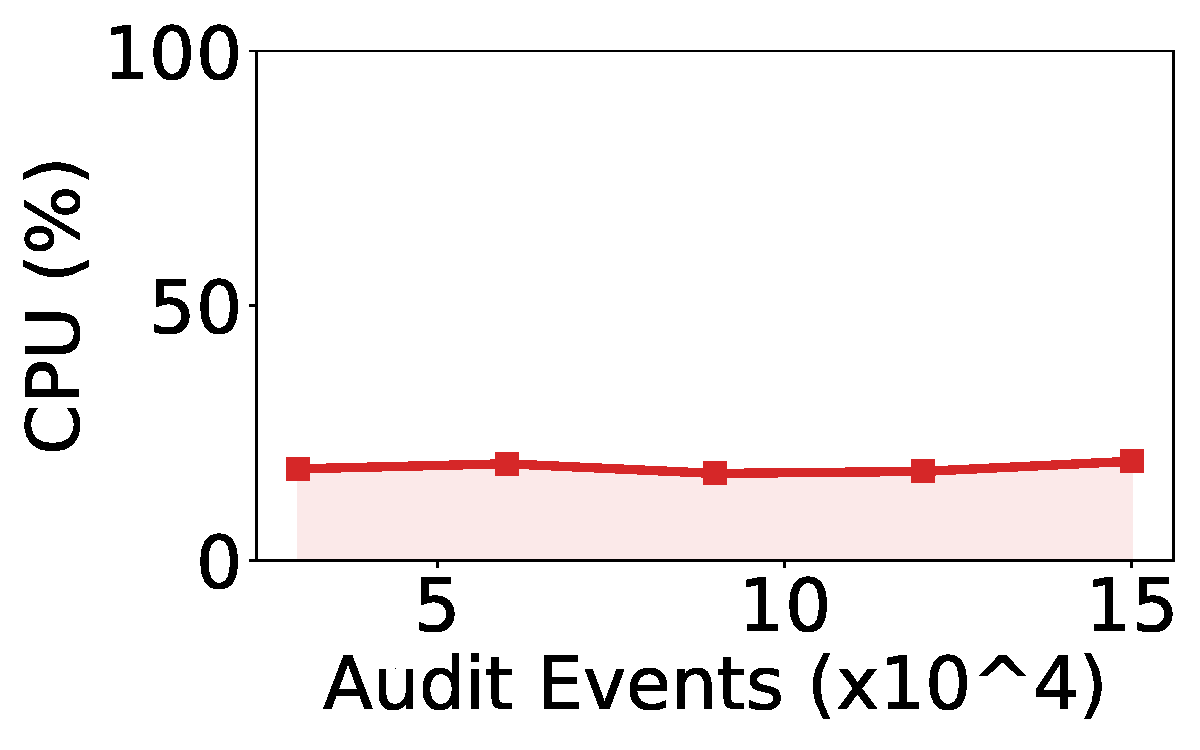
\includegraphics[width=0.20\textwidth]{fig/cpu.pdf}\label{cpu_client}}
%   \hfill
%   \subfloat[RAM utilization client side]{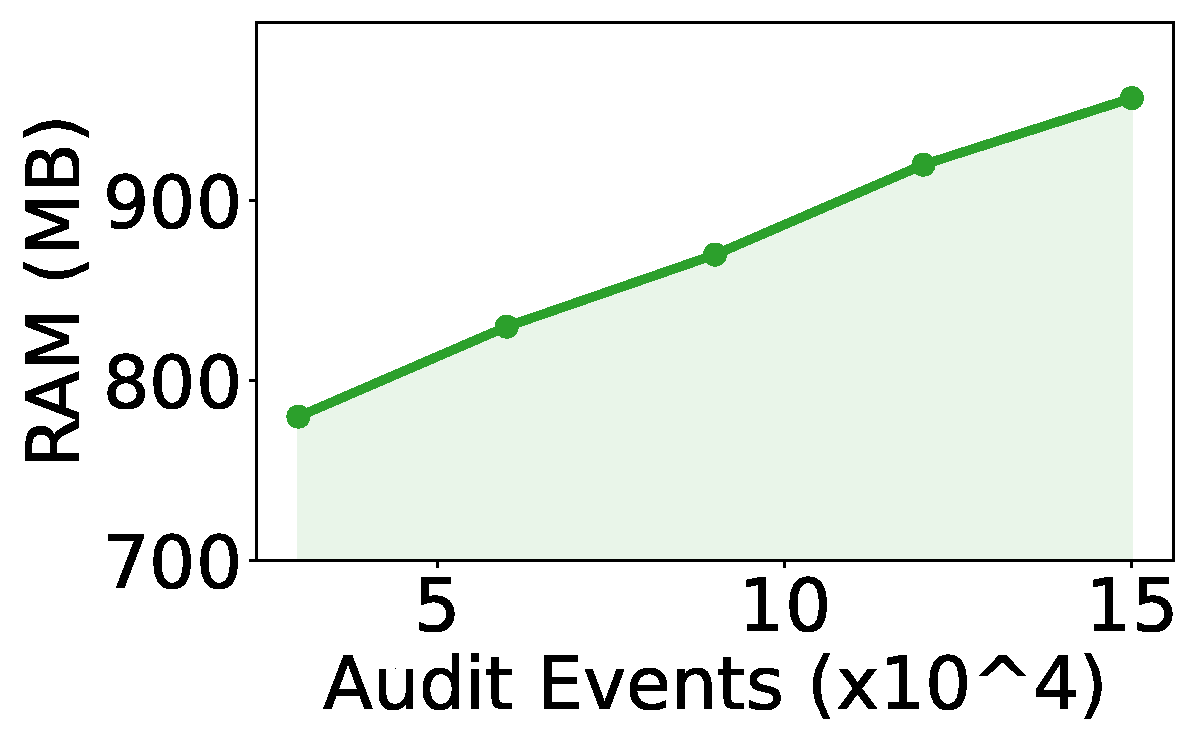
\includegraphics[width=0.20\textwidth]{fig/ram.pdf}\label{ram_client}}
%   \hfill
%   \subfloat[CPU utilization central server.]{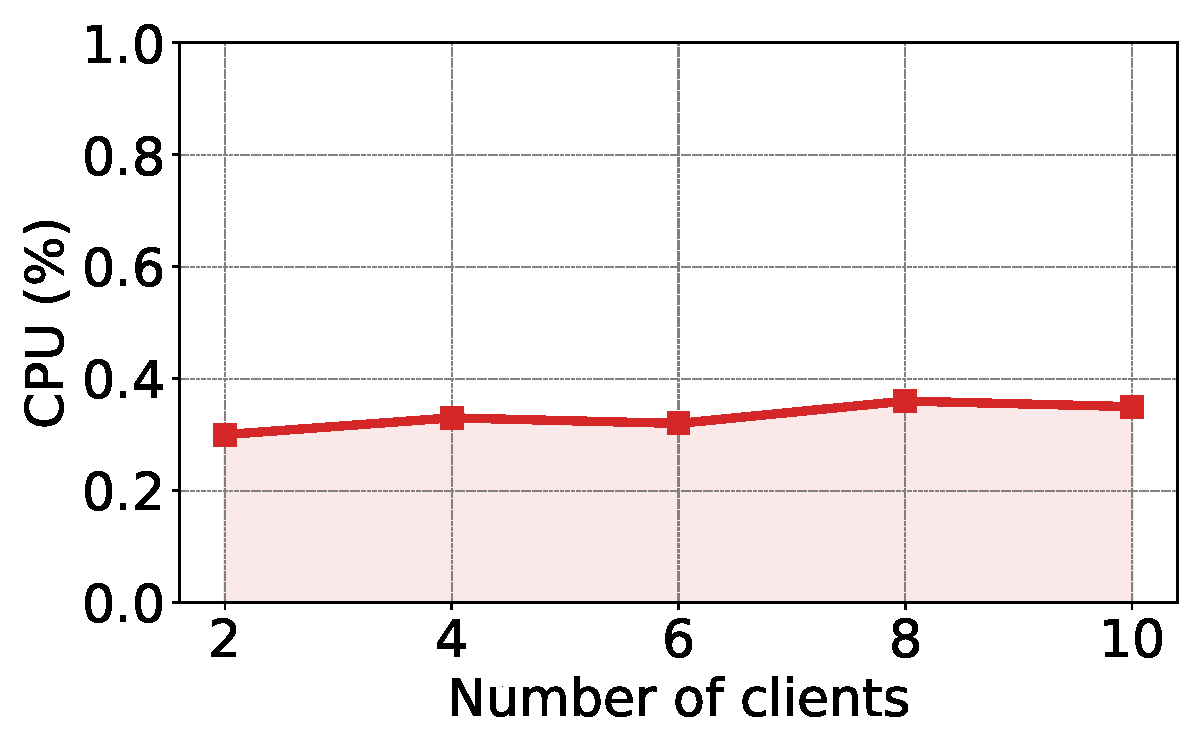
\includegraphics[width=0.20\textwidth]{fig/cpu_central.pdf}\label{cpu_central}}
%   \hfill
%   \subfloat[RAM utilization central server]{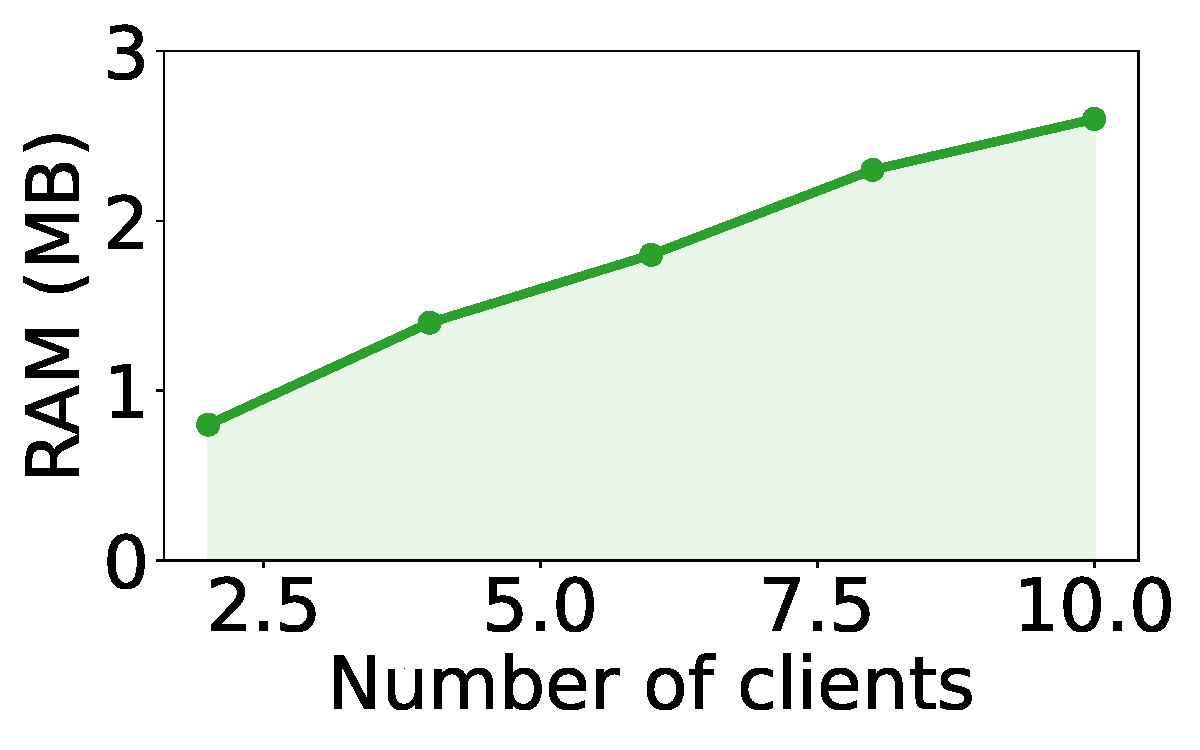
\includegraphics[width=0.20\textwidth]{fig/ram_central.pdf}\label{ram_central}}
%   \hfill
%   \subfloat[CPU utilization utility server.]{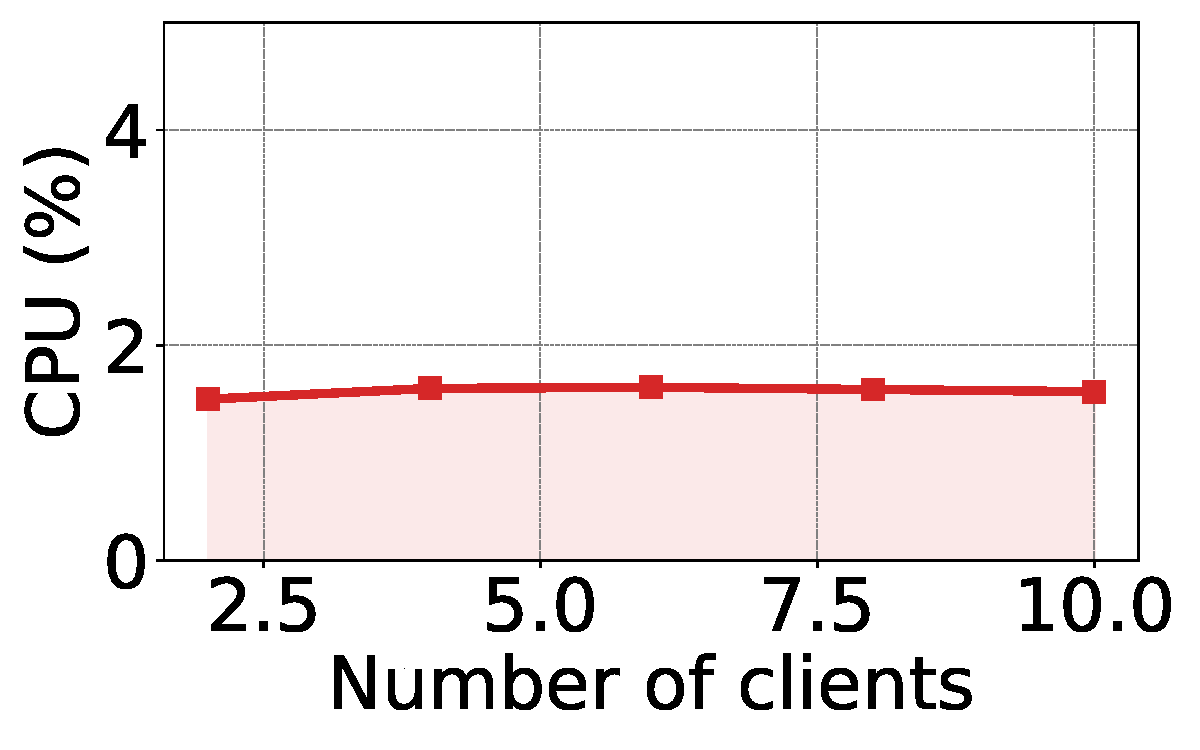
\includegraphics[width=0.20\textwidth]{fig/cpu_utility.pdf}\label{cpu_utility}}
%   \hfill
%   \subfloat[RAM utilization utility server]{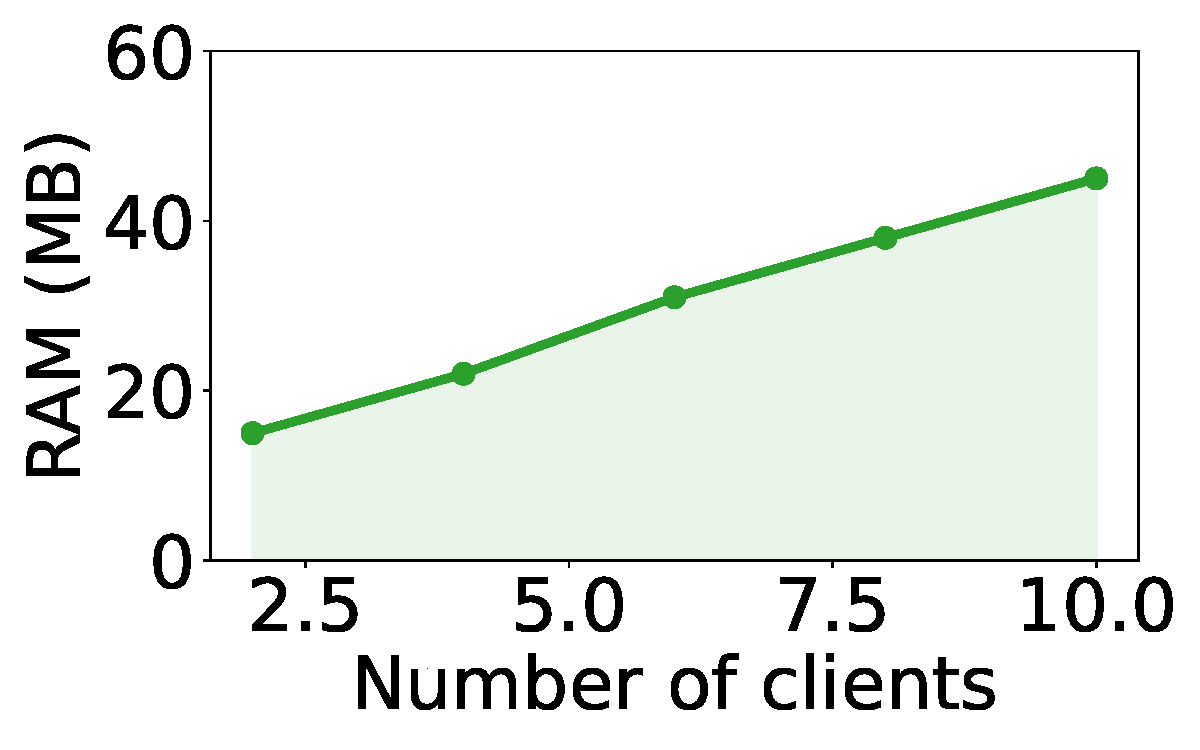
\includegraphics[width=0.20\textwidth]{fig/ram_utility.pdf}\label{ram_utility}}
%   \caption{Resource consumption of various components of \Sys.}
%   \label{fig:resource}
%   \vspace{-2ex}
% \end{figure}



% \subsection{Enterprise settings evaluation}
% \label{cost_metric}
% We examined the operational costs of deploying \Sys in comparison to centralized solutions like \flash and \kairos for organizational use. Our evaluation concentrates on two primary cost components: network expenses (\(C_{N}\)), and processing costs (\(C_{P}\)).

% \PP{Network Overhead:} We estimate this cost for the \flash and \kairos system using the \optc dataset. Each host within \optc produces approximately 1GB of audit logs daily, equating to nearly one million audit events. For an organization with 1,000 hosts, the total daily log volume would be 1,000 GB. This data volume necessitates transmission over the network to a central server operating the \pids. In contrast, \Sys achieves a significant reduction in these overheads. The only network expenses for \Sys arise from the transmission of the \gnnshort and \wordvec models; the \gnnshort model is roughly 13kb, while the average \wordvec model is 6 MB. Thus, the communication cost with the central server would be 12.70 MB, and for the utility server, it would be 5.86 GB. Ultimately, \Sys results in a 170-fold decrease in communication costs compared to \flash and \kairos.

% \PP{Processing Overhead:} Additionally, \flash processes one million events in about 100 seconds, implying that processing events from 1,000 clients would necessitate approximately 27.7 hours. In contrast, \kairos processes 57,000 events in 11.6 seconds, leading to a processing time of 204 seconds for one million events. Consequently, processing data from 1,000 clients with \kairos would require around 56.6 hours. Compared to existing systems, \Sys processes client logs in a decentralized manner and the total processing time is bounded by the client with the most log data; it will only take approximately 3 minutes to run inference on the complete \optc dataset. The central and utility servers conduct a simple mean operation on the models, taking only a few seconds.

% \PP{Overall Operating costs:} To calculate the daily operational costs of running these systems for a specific organization, we utilized the Google Cloud Platform's (GCP) pricing calculator~\cite{gcp}. The cost to operate \flash under the previously mentioned workload is estimated at \$135, with computing expenses accounting for \$100 and network costs comprising \$35. Given its longer processing duration, the operational cost for \kairos would be twice that of \flash. Compared to these systems, the operational cost of \Sys for 1,000 client machines would be approximately \$10 per day, marking a 13-fold reduction compared to \flash and a 26-fold reduction compared to \kairos.

% Scalability concerns are addressed in this section

\subsection{Scalability in Enterprise settings}
\label{cost_metric}
We analyzed the performance of our system in an enterprise setting using the \optc dataset, which includes a large number of host machines. We compared our system to centralized systems such as \flash and \kairos, focusing on important metrics including network and processing overhead. We also provide further discussion on scaling FL to massive enterprise networks in Appendix~\ref{state:explosion}.

\PP{Network Overhead:} We estimate this cost for the \flash and \kairos system using the \optc dataset. Each host within \optc produces approximately 1GB of audit logs daily, equating to nearly one million audit events. For an organization with 1,000 hosts, the total daily log volume would be 1,000 GB. This data volume necessitates transmission over the network to a central server operating the \pids. In contrast, \Sys achieves a significant reduction in these overheads. The only network expenses for \Sys arise from the transmission of the \gnnshort and \wordvec models; the \gnnshort model is roughly \modelsize, while the average \wordvec model is 6 MB. Thus, the communication cost with the central server would be 12.70 MB, and for the utility server, it would be 5.86 GB. Hence, the network latency of model communications in \Sys is minimal compared to centralized systems where the raw system logs need to be sent over the network. Ultimately, \Sys results in a 170-fold decrease in communication costs compared to centralized \pids.  

\PP{Processing Overhead:} Additionally, \flash processes one million events in about 100 seconds, implying that processing events from 1,000 clients would necessitate approximately 27.7 hours. In contrast, \kairos processes 57,000 events in 11.6 seconds, leading to a processing time of 204 seconds for one million events. Consequently, processing data from 1,000 clients with \kairos would require around 56.6 hours. Compared to existing systems, \Sys processes client logs in a decentralized manner and the total processing time is bounded by the client with the most log data; it will only take approximately 3 minutes to run inference on the complete \optc dataset. The central and utility servers conduct a simple mean operation on the models, taking only a few seconds.

% \subsection{Robustness against mimicry attacks}
% \label{sec:mimicry}

% We assessed the robustness of our system against the adversarial mimicry attack proposed by Goyal et al.~\cite{goyal2023sometimes} using the E3 dataset. The attack's objective is to generate embeddings for nodes in the attack graphs that are similar to those in the benign graph, thus evading detection. To achieve this, structures from benign nodes are integrated into the attack graph. Figure~\ref{mimicryattack} illustrates the experimental results, with the x-axis representing the number of benign structures added and the y-axis corresponding to anomaly scores for all attack nodes. The findings indicate that our detector maintains robustness against this attack; adding benign structures has minimal effect on the anomaly scores of the attack nodes. The superior robustness of \Sys can be attributed to our process-categorization-based ensemble \gnnshort architecture, wherein each model specializes in understanding the behavior of specific system entities. Thus, when the graph structure surrounding these entities changes, the models can easily detect these alterations.\footnote{In contrast, the \flash system relies on a downstream model using \gnnshort embeddings to detect malicious entities. Generalizing a single model across system entities can cause it to overlook critical details, making it vulnerable to mimicry attacks. As demonstrated by the authors, \flash initially experiences a drop in anomaly scores, increasing the likelihood of attack nodes evading detection, a vulnerability not present in our system.}

% \begin{figure}[!t]
%   \centering
%   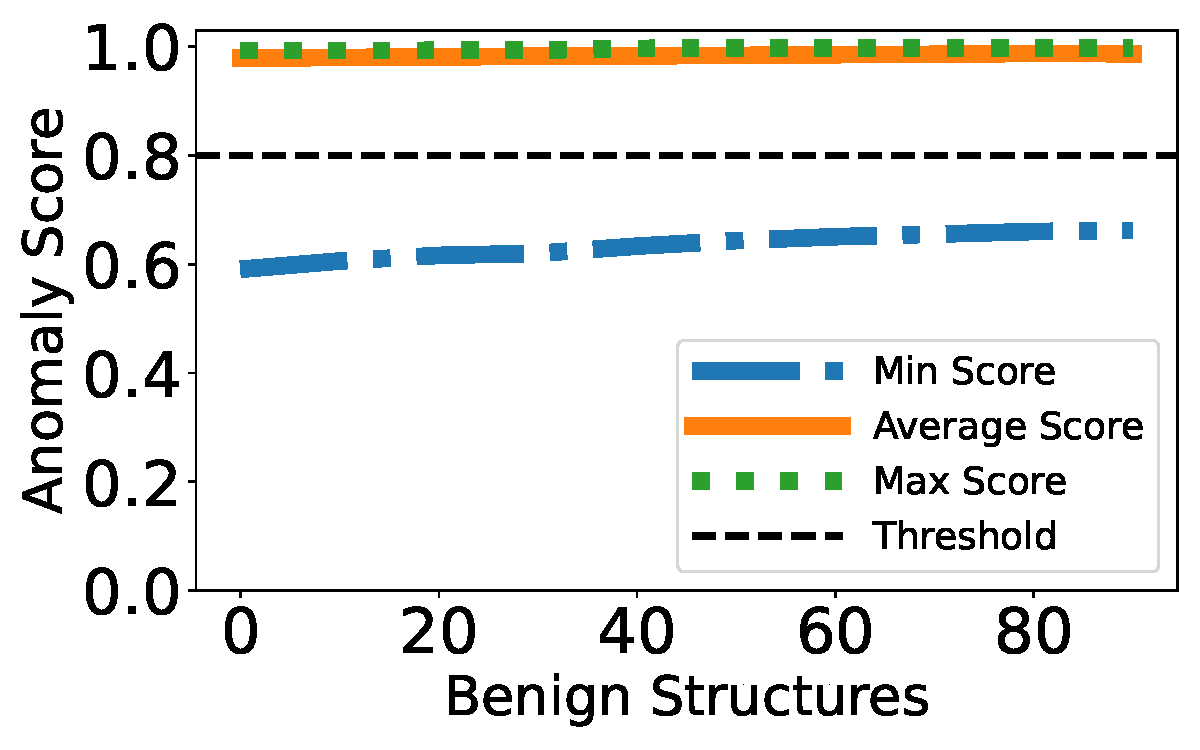
\includegraphics[width=0.4\textwidth]{fig/adversarial.pdf}
%   \caption{Adversarial mimicry attack analysis.}
%   \label{mimicryattack}
%   \vspace{-2ex}
% \end{figure}\


% \subsection{Effect of differential privacy on accuracy}

% Differential privacy is a method that can be combined with federated learning to offer protection against inference attacks~\cite{lyu2020threats,nasr2019comprehensive,zari2021efficient} at the cost of detection accuracy. We have analyzed the robustness of our system against these attacks in Section~\ref{privacy}. Here we will examine the impact of differential privacy noise levels on the detection performance of \Sys. Differential privacy achieves model privacy by adding a controlled amount of random noise to the model parameters, which helps in concealing the influence of any individual data point. In our context, differential privacy introduces a parameter called epsilon $\epsilon$ which dictates the intensity of noise added to the local \gnnshort model updates before they are aggregated at the central server for federated averaging, as detailed in Section~\ref{sec:methodology}.

% The parameter $\epsilon$ is crucial; it is inversely related to the amount of noise added -- lower values of $\epsilon$ result in higher noise levels, thereby increasing privacy but potentially degrading the utility of the model. Conversely, a higher $\epsilon$ indicates less noise, which may improve the model's detection capabilities but reduce privacy protection. By adjusting $\epsilon$ during the training phase, we assess the trade-off between privacy and detection performance in the globally trained models across various $\epsilon$ settings. Figure~\ref{epsvsscore} shows that increasing noise strength degrades model utility offering more privacy at the expense of reduced accuracy.

% \begin{figure}[!t]
%   \centering
%   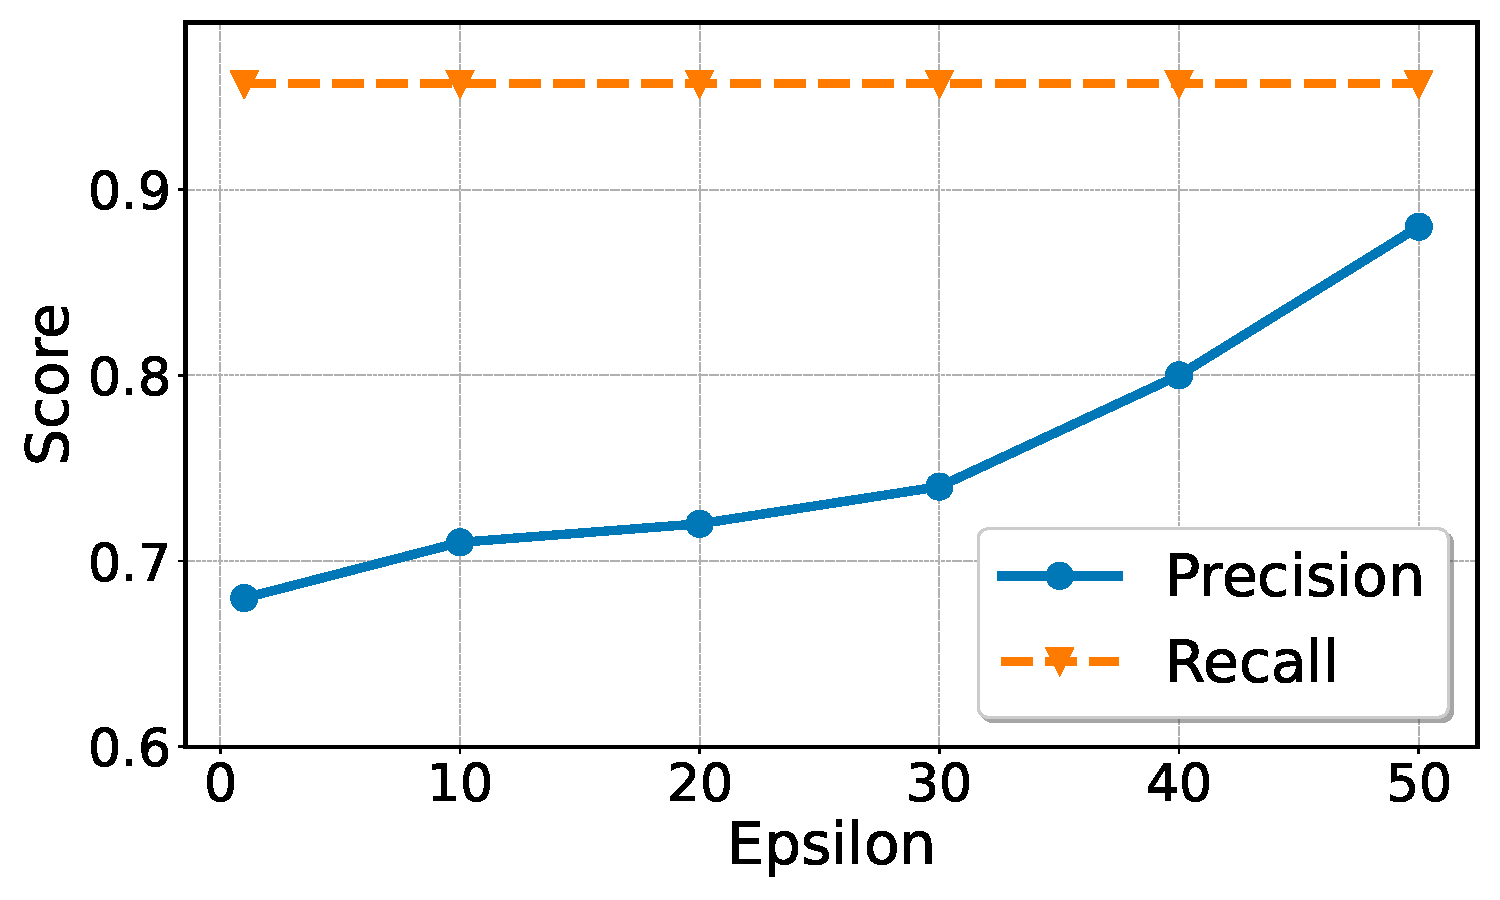
\includegraphics[width=0.25\textwidth]{fig/epsvsscore.pdf}
%   \caption{Effect of differential privacy noise on detection using E3 dataset. Note that we observed similar results on the other datasets.}
%   \label{epsvsscore}
%   \vspace{-2ex}
% \end{figure}


% \begin{figure*}[!t]
%   \centering
%   \subfloat[Anomaly threshold effect.]{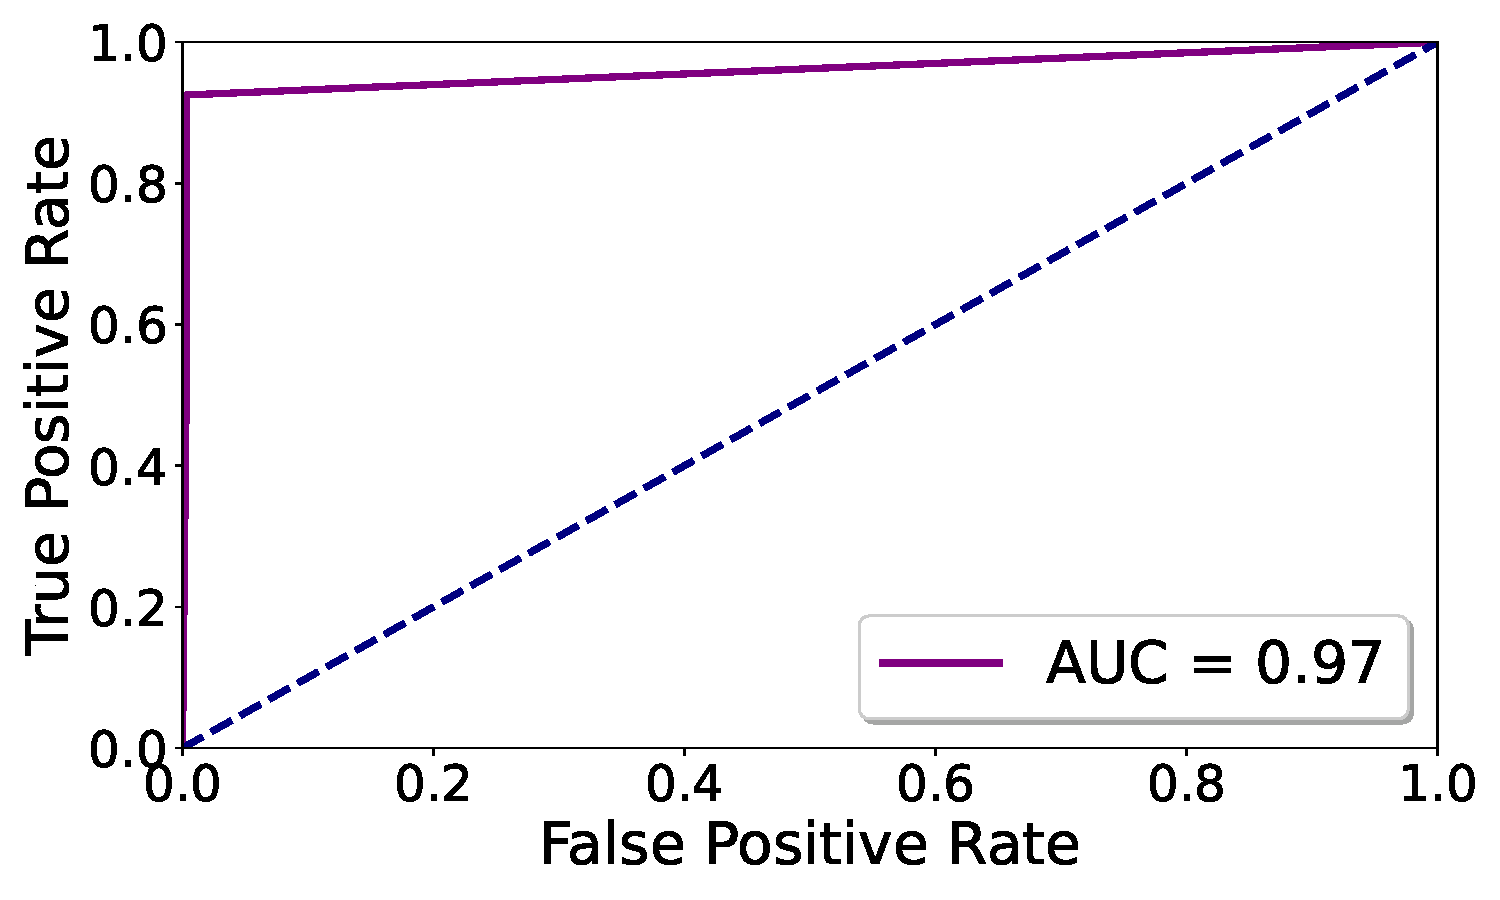
\includegraphics[width=0.24\textwidth]{fig/thresh.pdf}\label{thresh}}
%   \hfill
%   \subfloat[Effect of number of categories vs detection performance using E3 dataset.]{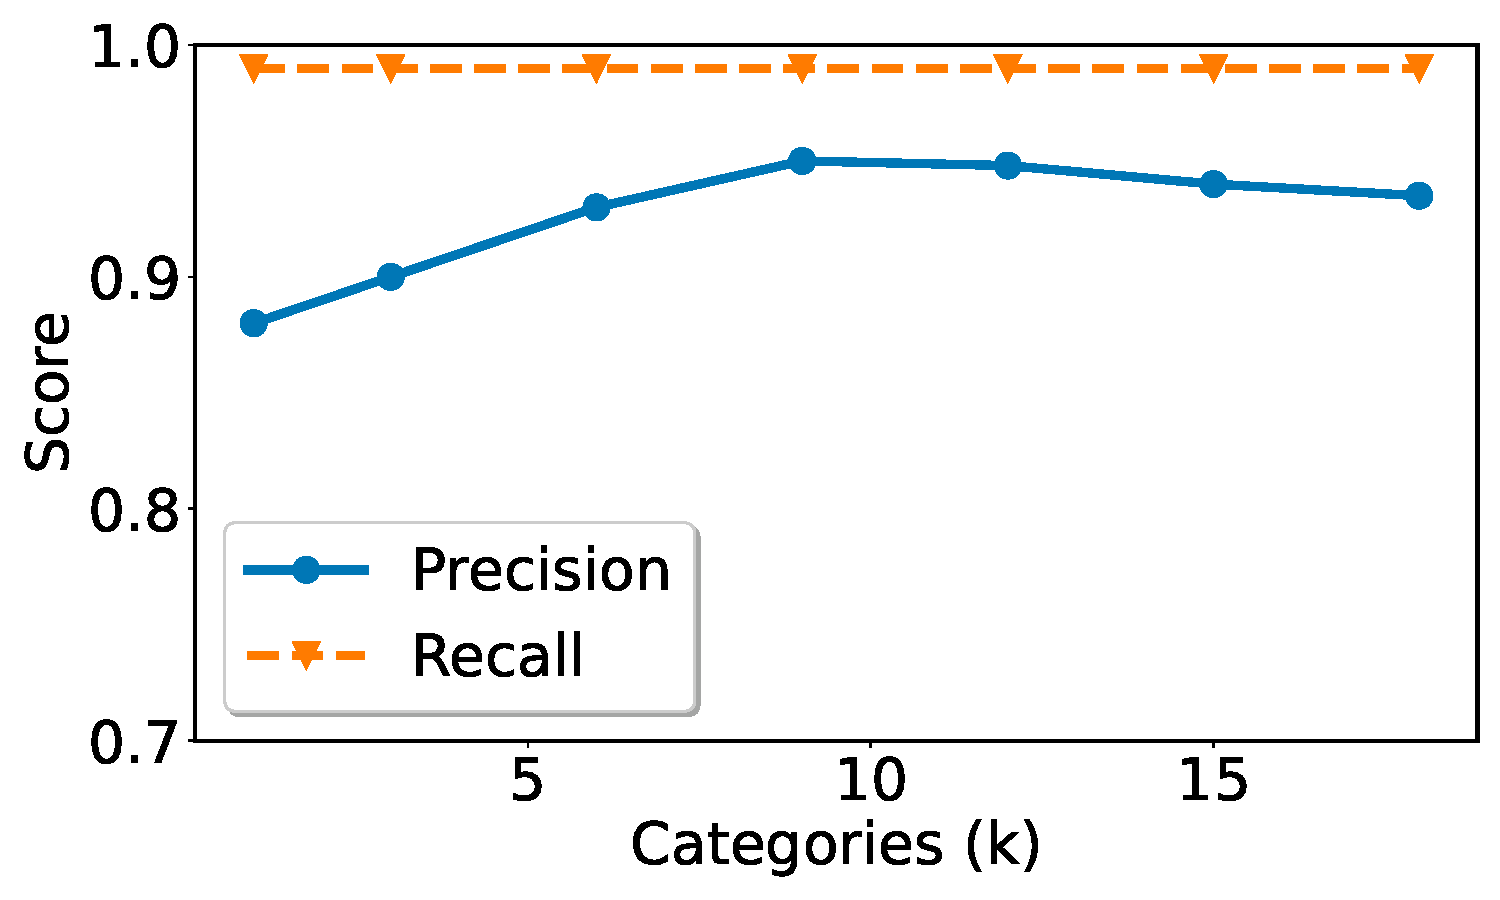
\includegraphics[width=0.24\textwidth]{fig/kvsscore.pdf}\label{catgvsscore}}
%   \hfill
%   \subfloat[Federated averaging rounds vs detection performance using E3 dataset.]{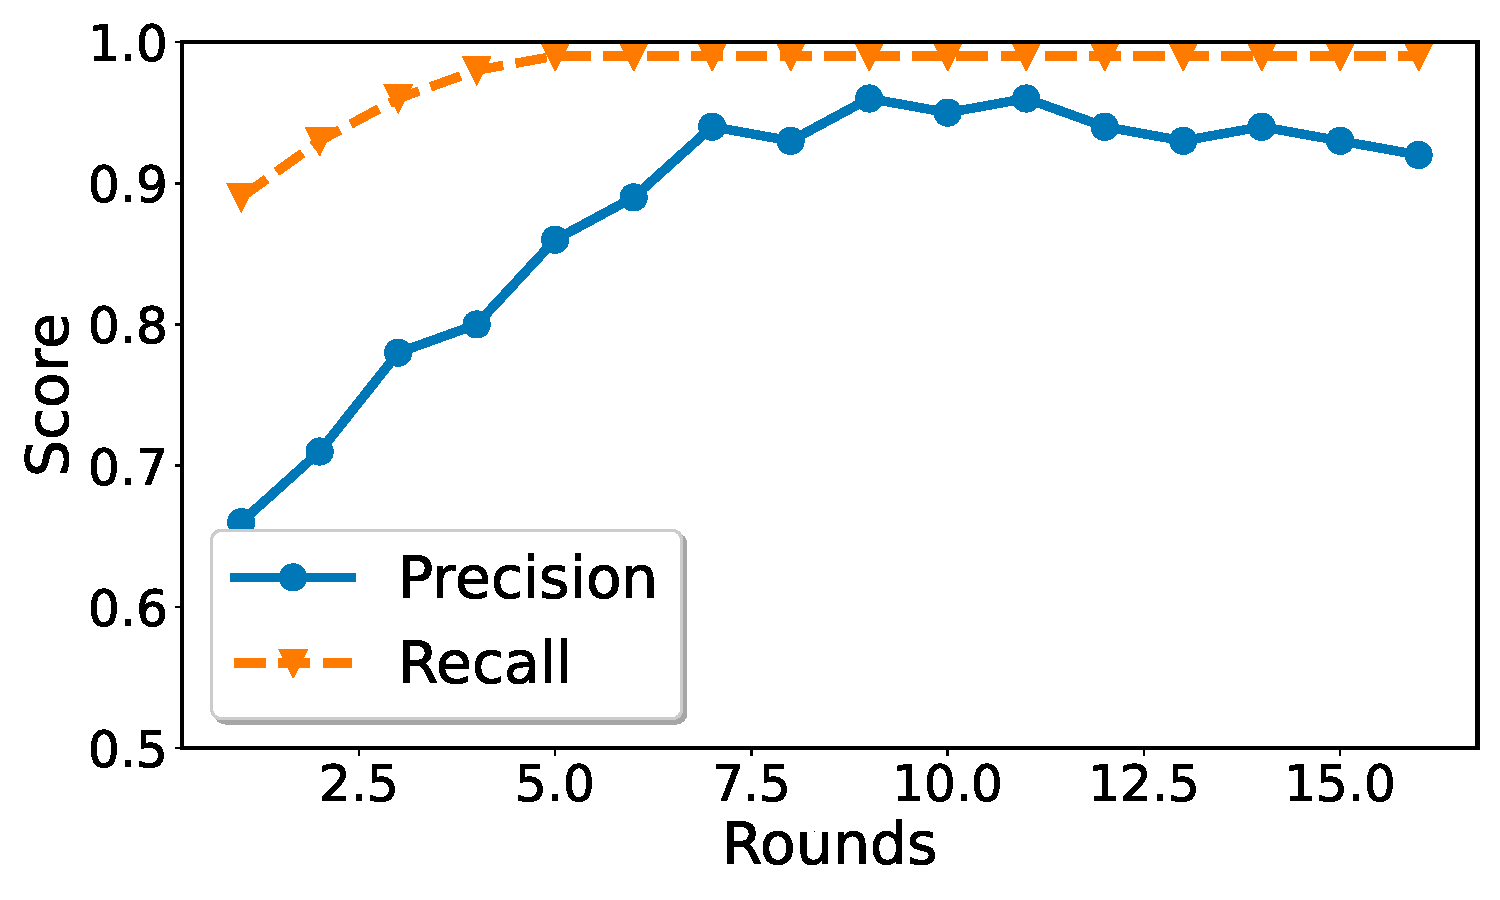
\includegraphics[width=0.24\textwidth]{fig/roundsvsscore.pdf}\label{roundsvsscore}}
%   \hfill
%   \subfloat[Effect of number of hosts vs detection metrics using \optc dataset]{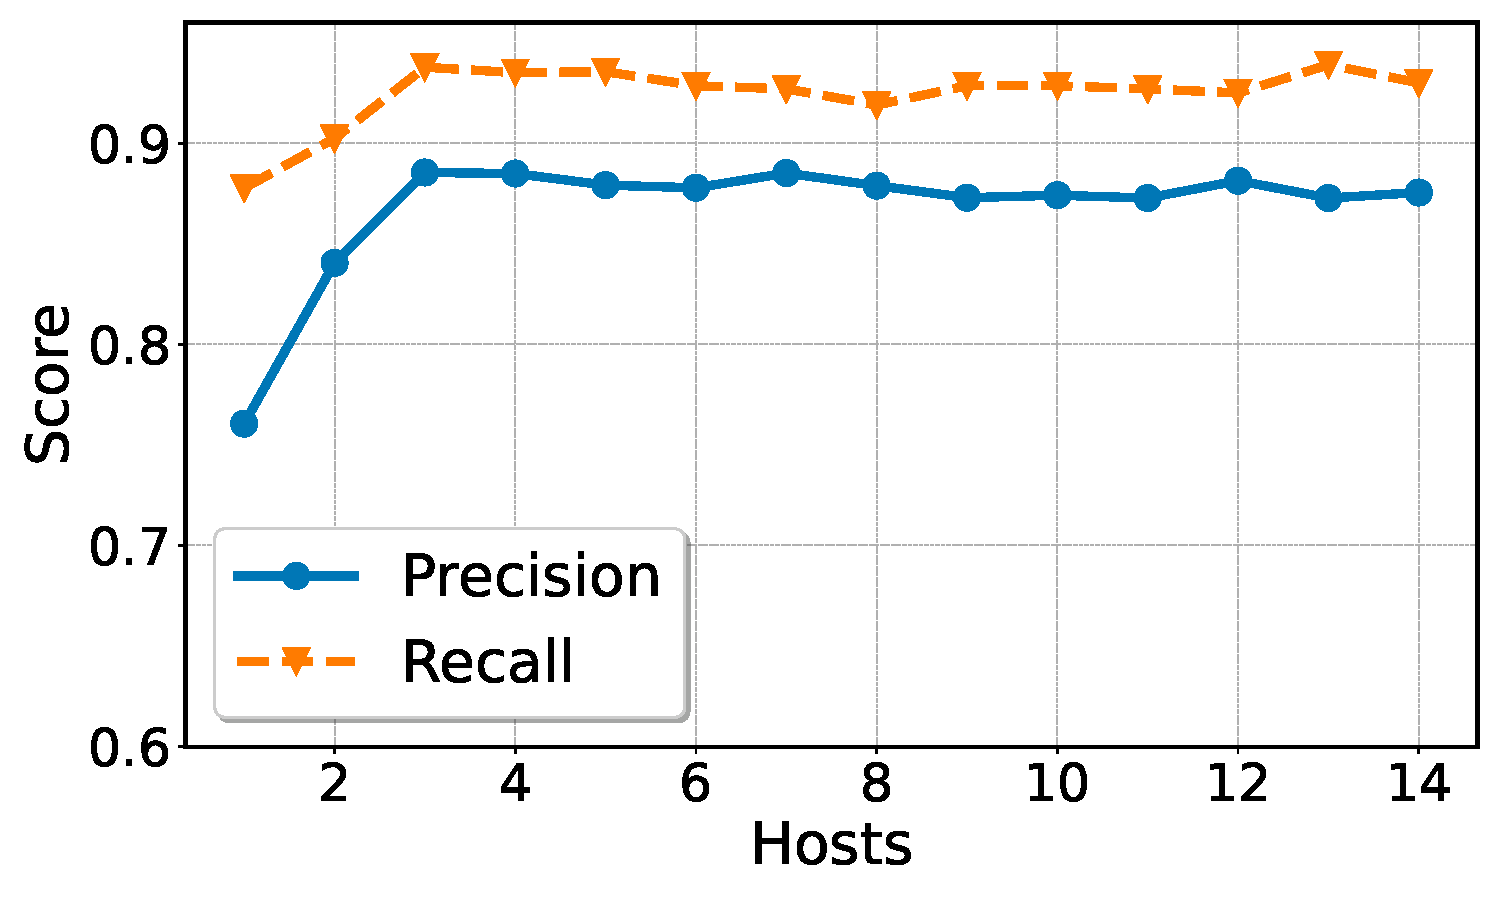
\includegraphics[width=0.24\textwidth]{fig/scoresvshosts.pdf}\label{rscoresvshosts}}
%   \caption{Ablation Study of various \Sys components.}
%   \label{ablation}
%   \vspace{-2ex}
% \end{figure*}

% \PP{Adversarial Attacks Analysis} We discussed robustness to mimicry attacks in Section~\ref{sec:mimicry}. Here, we address vulnerabilities to other types of adversarial attacks, including gradient-based attacks, model poisoning, and inference attacks (discussed in Section~\ref{sec:privacy}). Addressing these attacks is beyond the scope of this paper, as we focus on establishing an end-to-end framework for privacy-aware PIDS. We plan to integrate advancements in adversarial defense mechanisms against such attacks into \Sys to enhance its robustness in future work. These integrations are discussed below.

% Gradient-based adversarial attacks~\cite{chakraborty2021survey} typically require white-box access to the target machine learning model, including its parameters. This necessity often renders them impractical for real-world applications. In contrast, black-box attacks, which utilize iterative, query-based techniques, tend to be more detectable and complex to implement due to their conspicuous nature. Such attacks are feasible if an attacker manages to compromise a client machine. However, during the operational phase, a compromised client cannot affect other clients because they are working independently. Several existing defenses can be employed during model training to enhance the system's resilience against these attacks. Adversarial training~\cite{tramer2019adversarial} is one effective strategy, wherein the model is trained with perturbed input data to increase its robustness to such attacks.

% During the training phase, poisoning attacks executed by malicious actors may introduce corrupt weights to compromise the global model~\cite{jagielski2018manipulating}. To improve \Sys's resilience against such threats, several defensive methods can be used. Among these, advanced model aggregation methods, such as Multi-Krum~\cite{munoz2019byzantine}, can be particularly effective. This method employs clustering techniques on the central server to identify anomalous updates during model aggregation. Consequently, outlier updates are removed, enhancing the system's robustness against poisoning.

\subsection{RQ4: Adversarial Attacks Analysis}
\label{sec:adversarial}

% \wajih{would it be possible to combine Figure 4 and Figure 3 into one figure with three subflots/subfigures.}

% \begin{figure}[!t]
%   \centering
%   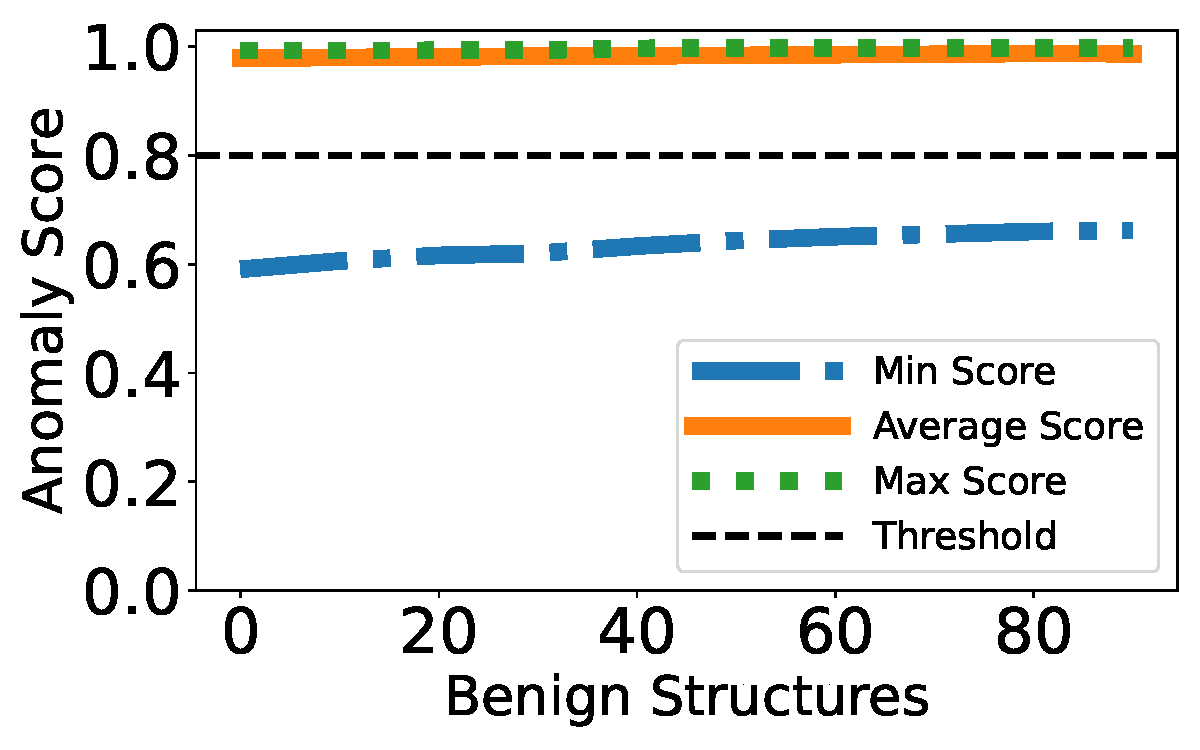
\includegraphics[width=0.34\textwidth]{fig/adversarial.pdf}
%   \caption{Adversarial mimicry attack analysis.}
%   \label{mimicryattack}
%   \vspace{-2ex}
% \end{figure}


In this section, we analyze the robustness of our system against mimicry, model poisoning, gradient-based attacks and bin-level inference attacks. Membership inference attacks are discussed in Section~\ref{sec:privacy}.

\begin{figure*}[!t]
  \centering
  \subfloat[Model poisoning: FedAvg aggregation.]{%
    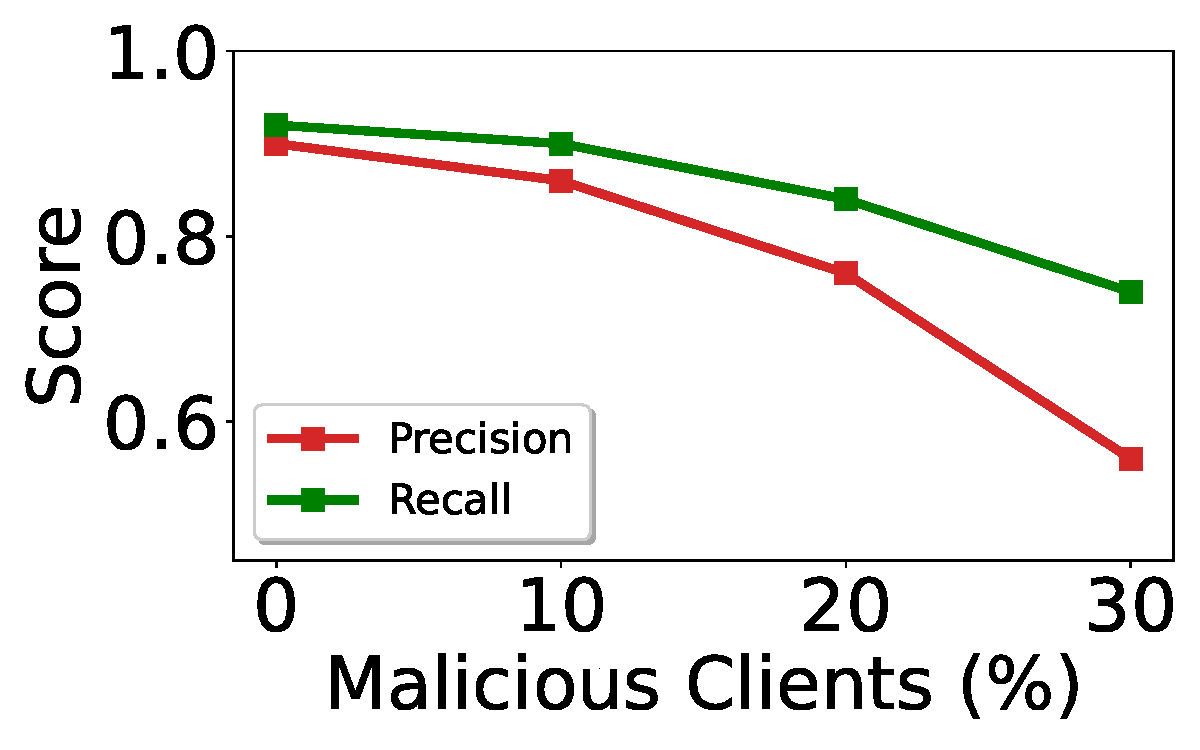
\includegraphics[height=0.15\textwidth]{fig/FedAvg_poisoning.pdf}%
    \label{fedavgpoison}
  }
  \hfill
  \subfloat[Model poisoning: Multi-Krum aggregation.]{%
    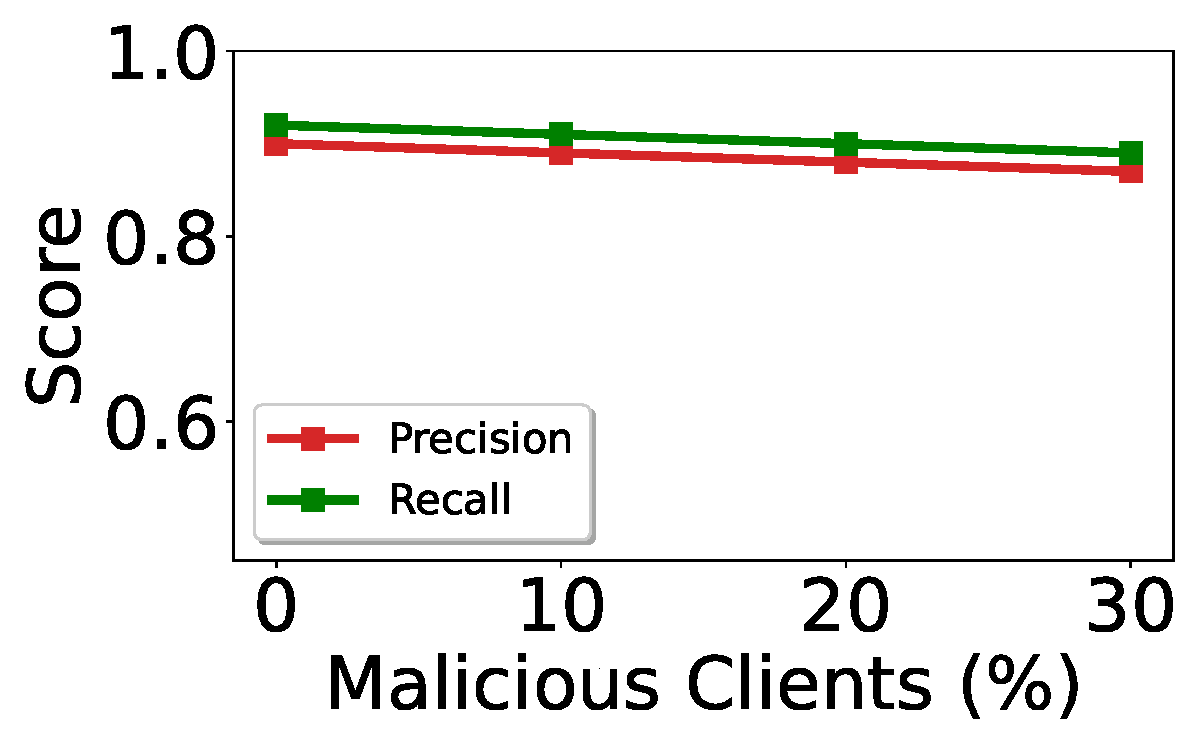
\includegraphics[height=0.15\textwidth]{fig/multi-krum.pdf}%
    \label{multikrumpoison}
  }
  \hfill
  \subfloat[Adversarial mimicry attack]{%
    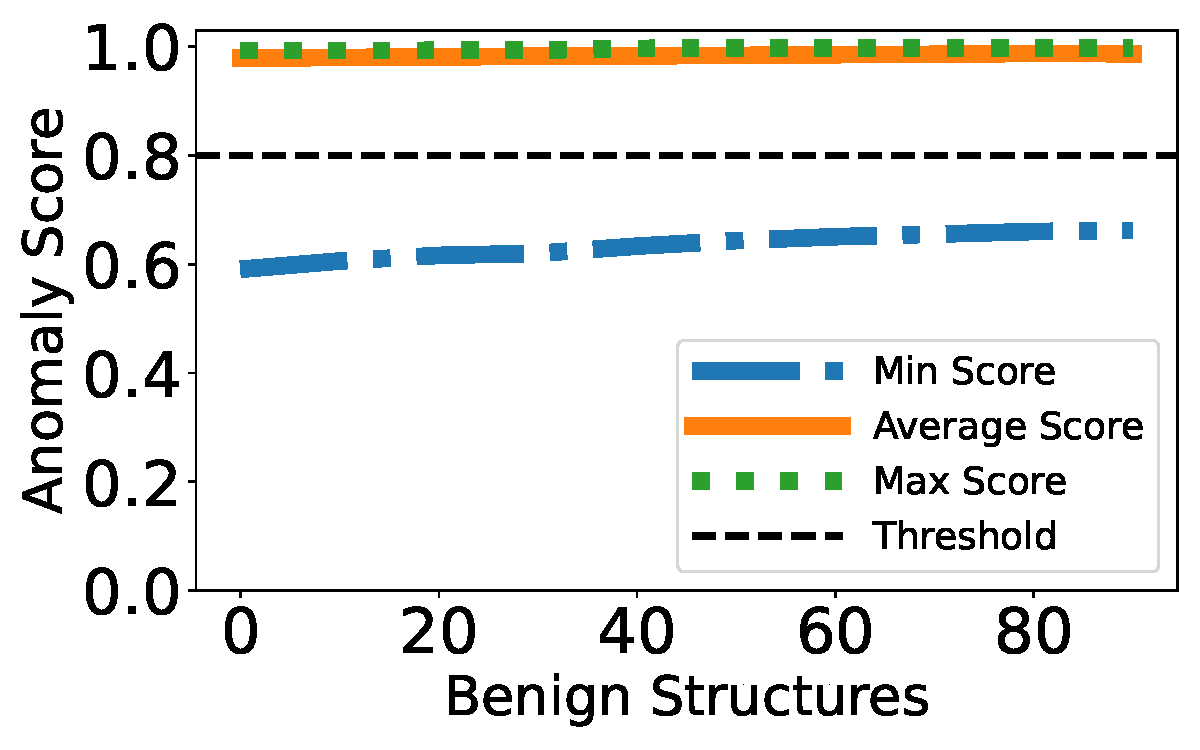
\includegraphics[height=0.15\textwidth]{fig/adversarial.pdf}%
    \label{mimicryattack}
  }
  \hfill
  \caption{Adversarial attacks analysis.}
  \label{fig:poison}
  \vspace{-3ex}
\end{figure*}

\PP{Mimicry Attacks}  We evaluated our system's resilience against the adversarial mimicry attack detailed by Goyal et al.~\cite{goyal2023sometimes} and compared its robustness with \flash. The attack aims to mimic benign graph embeddings, integrating benign node structures to evade detection. Using the E3 dataset, similar to \flash for fair comparison, our findings (shown in Figure~\ref{mimicryattack}) reveal that our detector remains robust; the integration of benign structures has a minimal impact on anomaly scores. Our system's superior robustness is due to our process-categorization-based ensemble \gnnshort architecture, which allows model specialization for different system entities, enhancing detection of structural changes. Conversely, \flash, relying on a generalized model for anomaly detection, exhibits vulnerabilities to mimicry attacks, as it may miss critical details. As demonstrated by the authors, \flash initially experiences a drop in anomaly scores, increasing the likelihood of attack nodes evading detection which is a vulnerability not present in our system. \footnote{PROVNINJA~\cite{mukherjee2023evading} is another mimicry attack that uses benign process profiles to find adversarial evasion strategies. It faces challenges against \pids like \flash and \Sys due to their multimodal architecture, which combines \wordvec for featurization and \gnnshort for anomaly detection. This complexity makes it difficult for attackers to create effective evasion strategies without accessing \wordvec directly or excessively querying the model, which conflicts with the black box nature of the assumed threat model of PROVNINJA.}


\PP{Model Poisoning Attacks} These occur when one or more malicious clients submit corrupted local model updates to the central server during training, thereby degrading the model’s performance. Existing methods typically assume an attack-free training phase, providing no defense against such attacks. We conducted experiments on the \optc dataset to assess the impact of poisoning attacks on our system, and we also evaluated how robust aggregation methods, such as Multi-Krum~\cite{munoz2019byzantine}, can enhance resilience.

Multi-Krum compares each client’s gradient with those of other clients, retaining only the most consistent updates. Since malicious updates must deviate significantly from benign ones to degrade performance, Multi-Krum effectively identifies and discards them as outliers. Figure~\ref{fig:poison} shows our experimental results using both FedAvg and Multi-Krum. With simple federated averaging, malicious noise critically affects the model by disrupting the benign distribution it learns. In contrast, Multi-Krum isolates and removes erroneous updates from malicious clients, preserving the global model. Notably, Multi-Krum assumes that fewer than one-third of all clients are malicious; therefore, in our experiments, we tested with a maximum of 30\% compromised clients.



\PP{Gradient-based Attacks} These attacks~\cite{chakraborty2021survey} exploit detailed knowledge of the target model, including its architecture and parameters, to calculate and apply malicious perturbations. Such white-box access allows an attacker to compute precise gradients that indicate how inputs should be modified to degrade the model’s performance. Other attacks tend to be black-box in nature, relying on iterative, query-based techniques to influence the model’s decisions. However, these repeated computations and queries run counter to the attacker’s aim of remaining inconspicuous, as they generate substantial activity and leave a significant footprint. Consequently, such attacks are often impractical in real-world scenarios. Several defenses can be employed during model training to bolster the system’s resilience against these threats. Adversarial training~\cite{tramer2019adversarial} is one effective strategy in which the model is trained on perturbed input data, thereby increasing its robustness against these attacks.

\PP{Bin-level Inference Attacks}  
In addition to the privacy risks outlined in Section~\ref{sec:privacy}, we identify another potential avenue for information leakage: bin-level inference attacks during training. In this scenario, a malicious client attempts to infer information about system entities held by other clients. It does so by manipulating the tokens it submits and observing changes in the utility server's harmonized vectors. Since overlapping token vectors are averaged, any noticeable change in the returned vector indicates that the token is shared across clients within the organization.  However, unlike the central and utility server inference risks, this attack does not compromise client identities and only the presence of a token in the system is revealed, preserving anonymity. Furthermore, our threat model~\ref{sec:threat}, consistent with prior \pids works, assumes a benign training environment free from adversarial clients. Bin-level inference attacks are thus only feasible during the training-time harmonization phase and not during deployment. We leave the development of federated learning methods robust to such adversarial training settings as an important direction for future work.

\section{Analysis of Privacy Protection}
\label{privacy}


\wajih{Use macros for common words in this whole section.}

\wajih{Be consistent with the terminology that you used in the abstract/intro.}

%\wajih{Make subsections if possible}

%\wajih{Look at Page 9 of the paper: "A federated graph neural network framework for privacy-preserving personaliz..." to see what to write here. }

%\wajih{If you read other privacy and FL paper you will similar sections/subsections in their paper. You can look at them to get some inspiration. Since we don't show in experiments that privacy is preserved. We need to theoretically prove that privacy is preserved. }

In this section, we analyze the preservation of user privacy within \(\Sys\), which is structured around three primary components: a central server, a utility server, and clients. The central server's role encompasses the application of federated averaging to the \(\gnnshort\) models received from clients.

The utility server performs contextual aggregation of semantic attribute vectors derived from clients' \(\wordvec\) models. The aggregation process can be represented as:
\[ V_{agg} = f(V_1, V_2, ..., V_n) \]
where \(V_{agg}\) denotes the aggregated vector, \(V_1, V_2, ..., V_n\) are the semantic attribute vectors from each client, and \(f\) is a mean aggregation function.

Clients are tasked with training the \(\wordvec\) and \(\gnnshort\) models on provenance graphs, these graphs are constructed from their local system audit logs. 

Within \(\Sys\), potential privacy compromises arise if either the central or utility server can infer specific details about individual clients' logs, such as the applications in use or particular attributes like filenames and IP addresses. Despite the central server's inability to access raw client data directly, it receives model updates from clients, thereby introducing a vulnerability to model inference attacks through analysis of these updates. Consider an attacker's objective to ascertain whether a system entity \(x\) with attributes \(y\) was utilized in training a client model \(m\). This necessitates the generation of multiple candidate node features for \(x\), taking into account various graph structures and interactions with other entities while considering diverse attributes. The search space for this task, \(S\), is extensive, spanning all conceivable processes, files, and network IPs. 

Assuming the server generates multiple candidate structures, it then requires access to the specific client's \(\wordvec\) model to generate feature vectors for these structures—a step prevented by the model's unavailability and inherent algorithmic randomness, rendering each training iteration of the \(\wordvec\) model distinct:
\[ F(x) = \wordvec(s_x) \]
where \(F(x)\) is the feature vector of structure \(x\) and \(s_x\) is the candidate sequence.

Consequently, the dual-server architecture and semantic featurization significantly limits the central server's capacity for inference attacks. The utility server's function of contextually aggregating semantic attribute vectors introduces another potential privacy concern if the server could deduce the entities these vectors represent. This risk is mitigated by the secure encryption of tokens using keys generated by the central server, which the utility server cannot access, ensuring privacy protection:
\[ V_{enc} = \text{Encrypt}(V_{agg}, K) \]
where \(V_{enc}\) is the encrypted aggregated vector, and \(K\) is the encryption key generated by the central server.

Furthermore, a malicious client attempting to utilize the global aggregate to infer the applications used across the organization faces similar constraints. Such an attack is limited by the client's lack of access to the semantic attribute vectors widespread across the organization, significantly narrowing the attack's feasibility. Therefore, the architecture of \(\Sys\) robustly defends against model inference attacks, affirming the system's capacity to preserve privacy. This resilience is predicated on the non-collusion assumption between the central and utility servers—a standard premise upheld by related works~\cite{roy2020crypte,wu2022federated}, thereby ensuring the system's high degree of privacy preservation.
% % \PP{Adversarial Attacks Analysis} We discussed robustness to mimicry attacks in Section~\ref{sec:mimicry}. Here, we address vulnerabilities to other types of adversarial attacks, including gradient-based attacks, model poisoning, and inference attacks (discussed in Section~\ref{sec:privacy}). Addressing these attacks is beyond the scope of this paper, as we focus on establishing an end-to-end framework for privacy-aware PIDS. We plan to integrate advancements in adversarial defense mechanisms against such attacks into \Sys to enhance its robustness in future work. These integrations are discussed below.

% Gradient-based adversarial attacks~\cite{chakraborty2021survey} typically require white-box access to the target machine learning model, including its parameters. This necessity often renders them impractical for real-world applications. In contrast, black-box attacks, which utilize iterative, query-based techniques, tend to be more detectable and complex to implement due to their conspicuous nature. Such attacks are feasible if an attacker manages to compromise a client machine. However, during the operational phase, a compromised client cannot affect other clients because they are working independently. Several existing defenses can be employed during model training to enhance the system's resilience against these attacks. Adversarial training~\cite{tramer2019adversarial} is one effective strategy, wherein the model is trained with perturbed input data to increase its robustness to such attacks.

% During the training phase, poisoning attacks executed by malicious actors may introduce corrupt weights to compromise the global model~\cite{jagielski2018manipulating}. To improve \Sys's resilience against such threats, several defensive methods can be used. Among these, advanced model aggregation methods, such as Multi-Krum~\cite{munoz2019byzantine}, can be particularly effective. This method employs clustering techniques on the central server to identify anomalous updates during model aggregation. Consequently, outlier updates are removed, enhancing the system's robustness against poisoning.

\subsection{RQ4: Adversarial Attacks Analysis}
\label{sec:adversarial}

% \wajih{would it be possible to combine Figure 4 and Figure 3 into one figure with three subflots/subfigures.}

% \begin{figure}[!t]
%   \centering
%   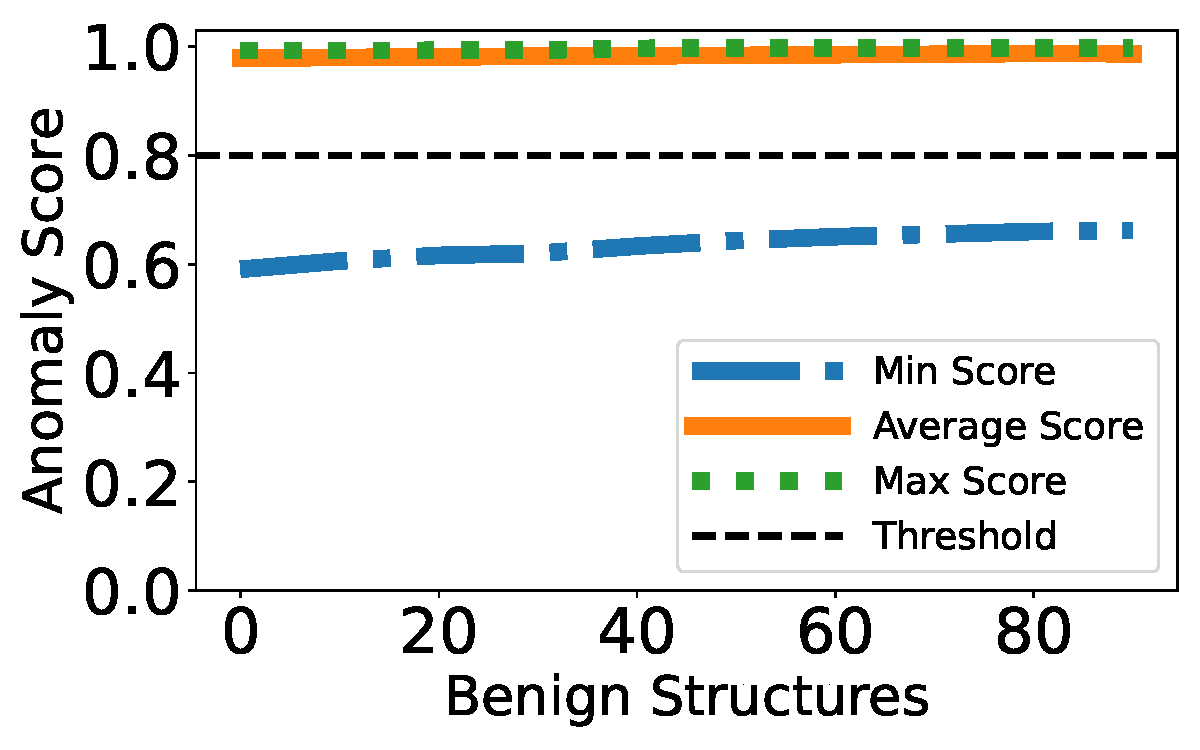
\includegraphics[width=0.34\textwidth]{fig/adversarial.pdf}
%   \caption{Adversarial mimicry attack analysis.}
%   \label{mimicryattack}
%   \vspace{-2ex}
% \end{figure}


In this section, we analyze the robustness of our system against mimicry, model poisoning, gradient-based attacks and bin-level inference attacks. Membership inference attacks are discussed in Section~\ref{sec:privacy}.

\begin{figure*}[!t]
  \centering
  \subfloat[Model poisoning: FedAvg aggregation.]{%
    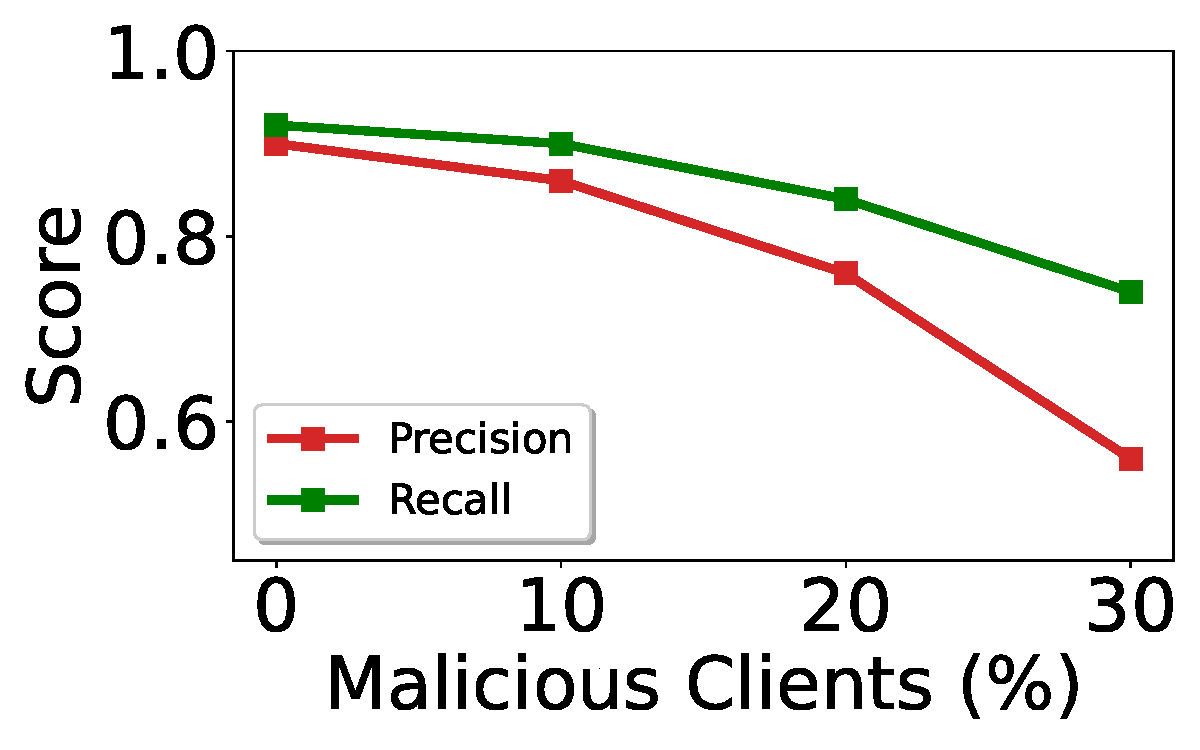
\includegraphics[height=0.15\textwidth]{fig/FedAvg_poisoning.pdf}%
    \label{fedavgpoison}
  }
  \hfill
  \subfloat[Model poisoning: Multi-Krum aggregation.]{%
    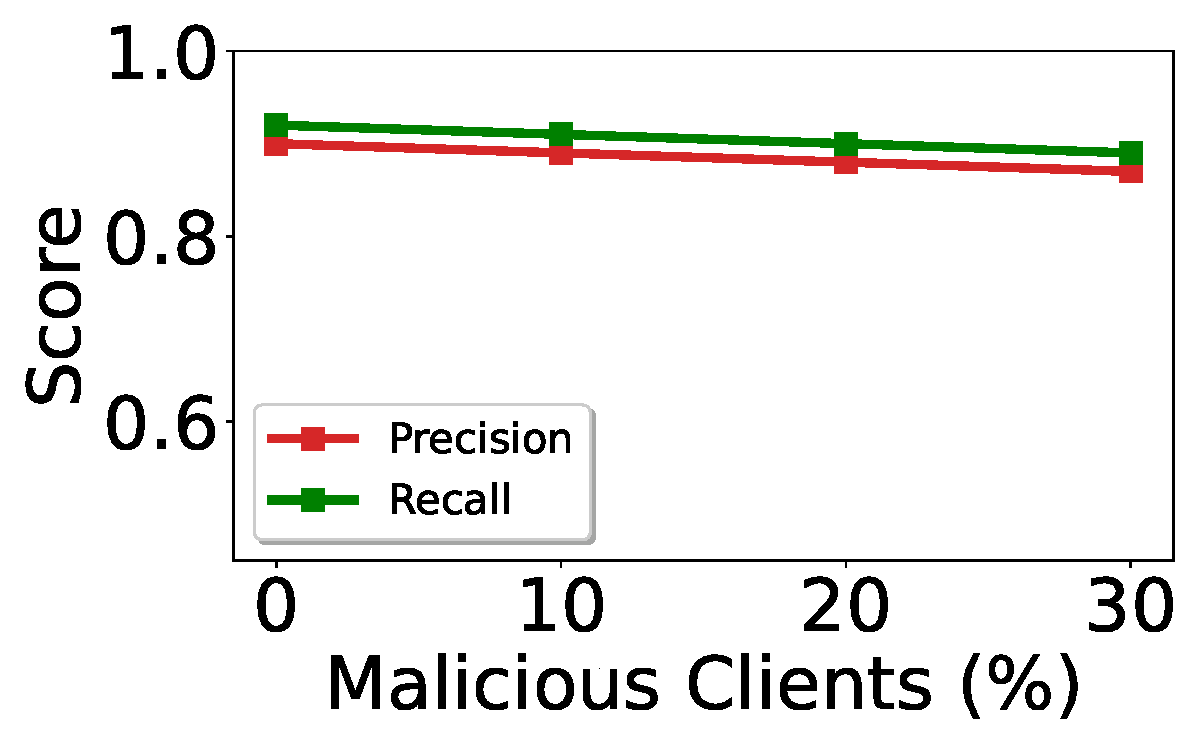
\includegraphics[height=0.15\textwidth]{fig/multi-krum.pdf}%
    \label{multikrumpoison}
  }
  \hfill
  \subfloat[Adversarial mimicry attack]{%
    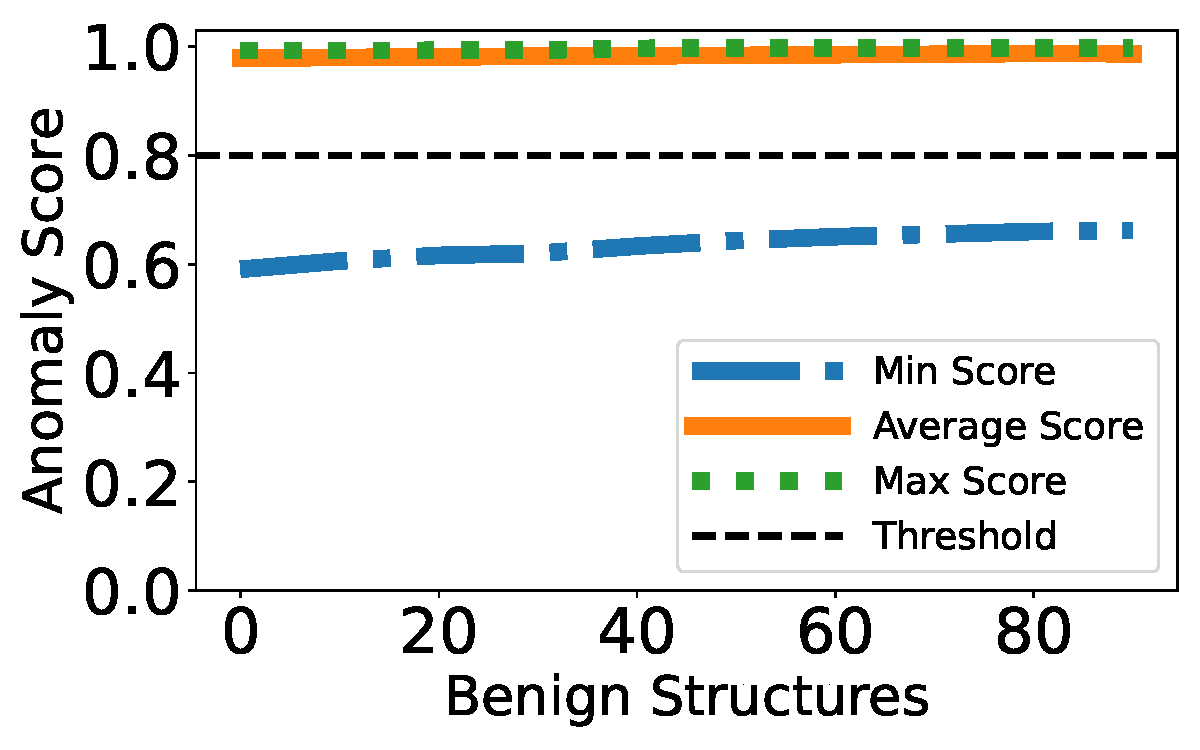
\includegraphics[height=0.15\textwidth]{fig/adversarial.pdf}%
    \label{mimicryattack}
  }
  \hfill
  \caption{Adversarial attacks analysis.}
  \label{fig:poison}
  \vspace{-3ex}
\end{figure*}

\PP{Mimicry Attacks}  We evaluated our system's resilience against the adversarial mimicry attack detailed by Goyal et al.~\cite{goyal2023sometimes} and compared its robustness with \flash. The attack aims to mimic benign graph embeddings, integrating benign node structures to evade detection. Using the E3 dataset, similar to \flash for fair comparison, our findings (shown in Figure~\ref{mimicryattack}) reveal that our detector remains robust; the integration of benign structures has a minimal impact on anomaly scores. Our system's superior robustness is due to our process-categorization-based ensemble \gnnshort architecture, which allows model specialization for different system entities, enhancing detection of structural changes. Conversely, \flash, relying on a generalized model for anomaly detection, exhibits vulnerabilities to mimicry attacks, as it may miss critical details. As demonstrated by the authors, \flash initially experiences a drop in anomaly scores, increasing the likelihood of attack nodes evading detection which is a vulnerability not present in our system. \footnote{PROVNINJA~\cite{mukherjee2023evading} is another mimicry attack that uses benign process profiles to find adversarial evasion strategies. It faces challenges against \pids like \flash and \Sys due to their multimodal architecture, which combines \wordvec for featurization and \gnnshort for anomaly detection. This complexity makes it difficult for attackers to create effective evasion strategies without accessing \wordvec directly or excessively querying the model, which conflicts with the black box nature of the assumed threat model of PROVNINJA.}


\PP{Model Poisoning Attacks} These occur when one or more malicious clients submit corrupted local model updates to the central server during training, thereby degrading the model’s performance. Existing methods typically assume an attack-free training phase, providing no defense against such attacks. We conducted experiments on the \optc dataset to assess the impact of poisoning attacks on our system, and we also evaluated how robust aggregation methods, such as Multi-Krum~\cite{munoz2019byzantine}, can enhance resilience.

Multi-Krum compares each client’s gradient with those of other clients, retaining only the most consistent updates. Since malicious updates must deviate significantly from benign ones to degrade performance, Multi-Krum effectively identifies and discards them as outliers. Figure~\ref{fig:poison} shows our experimental results using both FedAvg and Multi-Krum. With simple federated averaging, malicious noise critically affects the model by disrupting the benign distribution it learns. In contrast, Multi-Krum isolates and removes erroneous updates from malicious clients, preserving the global model. Notably, Multi-Krum assumes that fewer than one-third of all clients are malicious; therefore, in our experiments, we tested with a maximum of 30\% compromised clients.



\PP{Gradient-based Attacks} These attacks~\cite{chakraborty2021survey} exploit detailed knowledge of the target model, including its architecture and parameters, to calculate and apply malicious perturbations. Such white-box access allows an attacker to compute precise gradients that indicate how inputs should be modified to degrade the model’s performance. Other attacks tend to be black-box in nature, relying on iterative, query-based techniques to influence the model’s decisions. However, these repeated computations and queries run counter to the attacker’s aim of remaining inconspicuous, as they generate substantial activity and leave a significant footprint. Consequently, such attacks are often impractical in real-world scenarios. Several defenses can be employed during model training to bolster the system’s resilience against these threats. Adversarial training~\cite{tramer2019adversarial} is one effective strategy in which the model is trained on perturbed input data, thereby increasing its robustness against these attacks.

\PP{Bin-level Inference Attacks}  
In addition to the privacy risks outlined in Section~\ref{sec:privacy}, we identify another potential avenue for information leakage: bin-level inference attacks during training. In this scenario, a malicious client attempts to infer information about system entities held by other clients. It does so by manipulating the tokens it submits and observing changes in the utility server's harmonized vectors. Since overlapping token vectors are averaged, any noticeable change in the returned vector indicates that the token is shared across clients within the organization.  However, unlike the central and utility server inference risks, this attack does not compromise client identities and only the presence of a token in the system is revealed, preserving anonymity. Furthermore, our threat model~\ref{sec:threat}, consistent with prior \pids works, assumes a benign training environment free from adversarial clients. Bin-level inference attacks are thus only feasible during the training-time harmonization phase and not during deployment. We leave the development of federated learning methods robust to such adversarial training settings as an important direction for future work.

\section{Discussion \& Limitations}
\label{sec:discussion}

%\wajih{Use macros for common words in this whole section.}

%\wajih{Be consistent with the terminology that you used in the abstract/intro.}

%\wajih{Move adversarial attacks in a separate section.}

%% \PP{Adversarial Attacks Analysis} We discussed robustness to mimicry attacks in Section~\ref{sec:mimicry}. Here, we address vulnerabilities to other types of adversarial attacks, including gradient-based attacks, model poisoning, and inference attacks (discussed in Section~\ref{sec:privacy}). Addressing these attacks is beyond the scope of this paper, as we focus on establishing an end-to-end framework for privacy-aware PIDS. We plan to integrate advancements in adversarial defense mechanisms against such attacks into \Sys to enhance its robustness in future work. These integrations are discussed below.

% Gradient-based adversarial attacks~\cite{chakraborty2021survey} typically require white-box access to the target machine learning model, including its parameters. This necessity often renders them impractical for real-world applications. In contrast, black-box attacks, which utilize iterative, query-based techniques, tend to be more detectable and complex to implement due to their conspicuous nature. Such attacks are feasible if an attacker manages to compromise a client machine. However, during the operational phase, a compromised client cannot affect other clients because they are working independently. Several existing defenses can be employed during model training to enhance the system's resilience against these attacks. Adversarial training~\cite{tramer2019adversarial} is one effective strategy, wherein the model is trained with perturbed input data to increase its robustness to such attacks.

% During the training phase, poisoning attacks executed by malicious actors may introduce corrupt weights to compromise the global model~\cite{jagielski2018manipulating}. To improve \Sys's resilience against such threats, several defensive methods can be used. Among these, advanced model aggregation methods, such as Multi-Krum~\cite{munoz2019byzantine}, can be particularly effective. This method employs clustering techniques on the central server to identify anomalous updates during model aggregation. Consequently, outlier updates are removed, enhancing the system's robustness against poisoning.

\subsection{RQ4: Adversarial Attacks Analysis}
\label{sec:adversarial}

% \wajih{would it be possible to combine Figure 4 and Figure 3 into one figure with three subflots/subfigures.}

% \begin{figure}[!t]
%   \centering
%   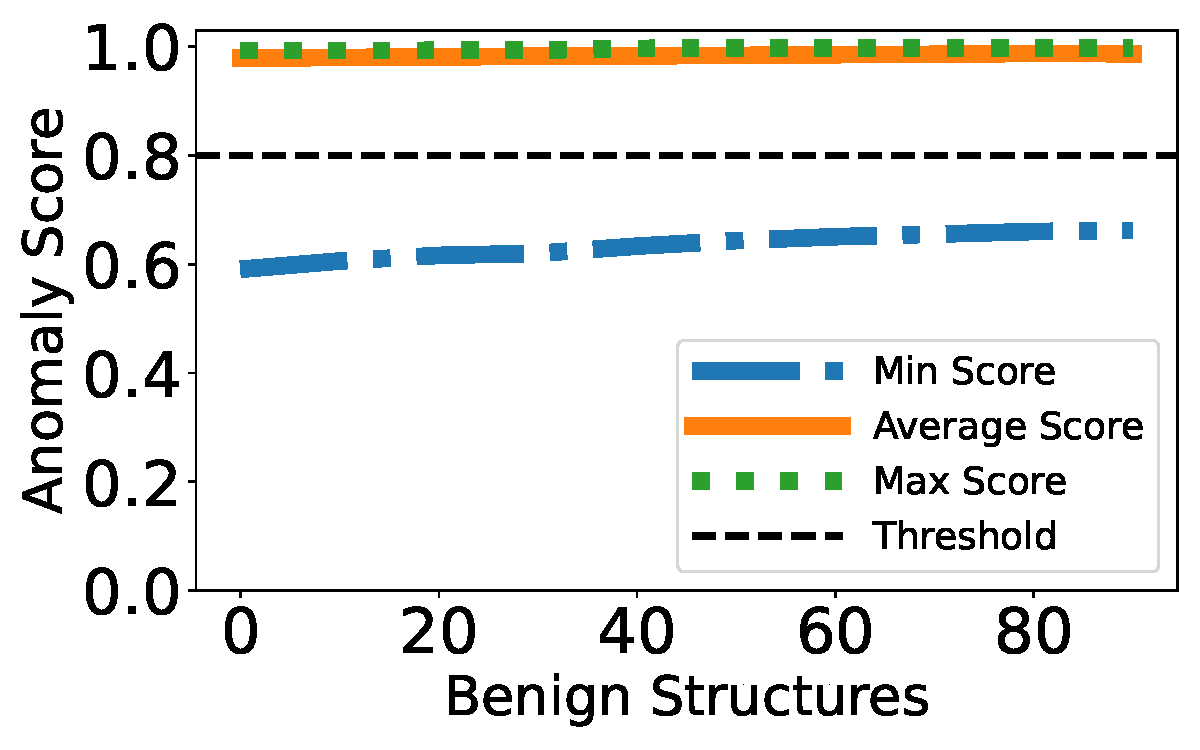
\includegraphics[width=0.34\textwidth]{fig/adversarial.pdf}
%   \caption{Adversarial mimicry attack analysis.}
%   \label{mimicryattack}
%   \vspace{-2ex}
% \end{figure}


In this section, we analyze the robustness of our system against mimicry, model poisoning, gradient-based attacks and bin-level inference attacks. Membership inference attacks are discussed in Section~\ref{sec:privacy}.

\begin{figure*}[!t]
  \centering
  \subfloat[Model poisoning: FedAvg aggregation.]{%
    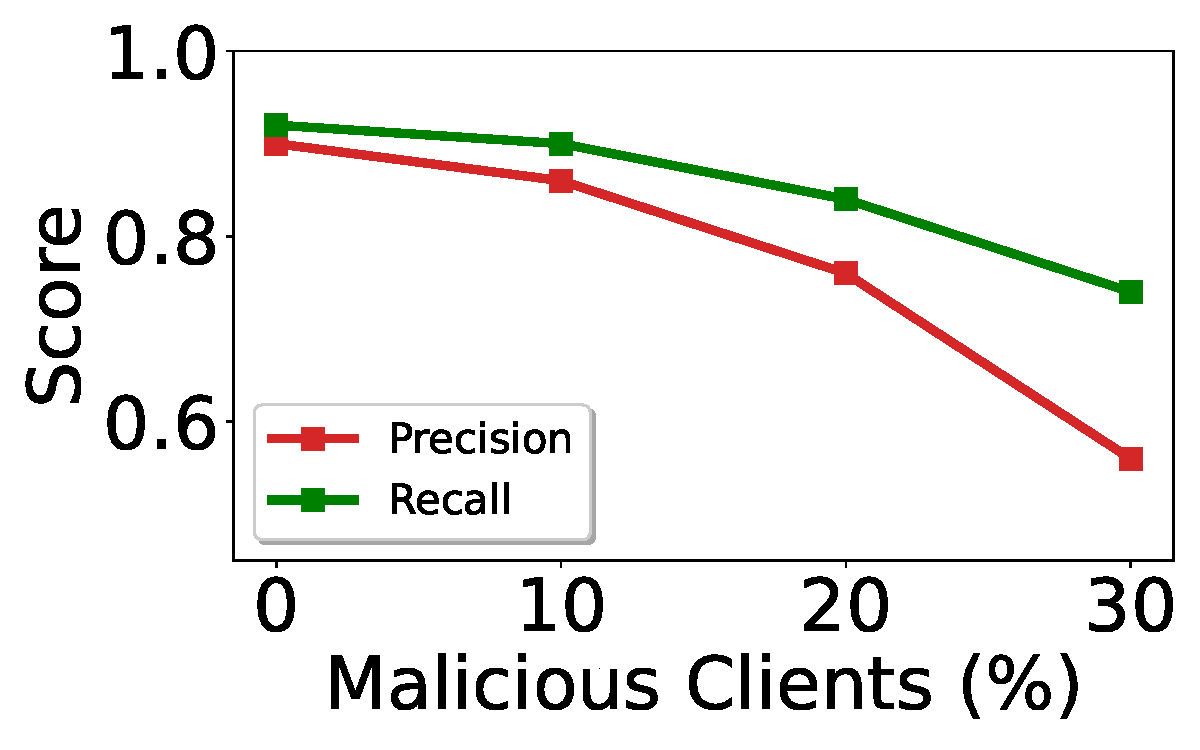
\includegraphics[height=0.15\textwidth]{fig/FedAvg_poisoning.pdf}%
    \label{fedavgpoison}
  }
  \hfill
  \subfloat[Model poisoning: Multi-Krum aggregation.]{%
    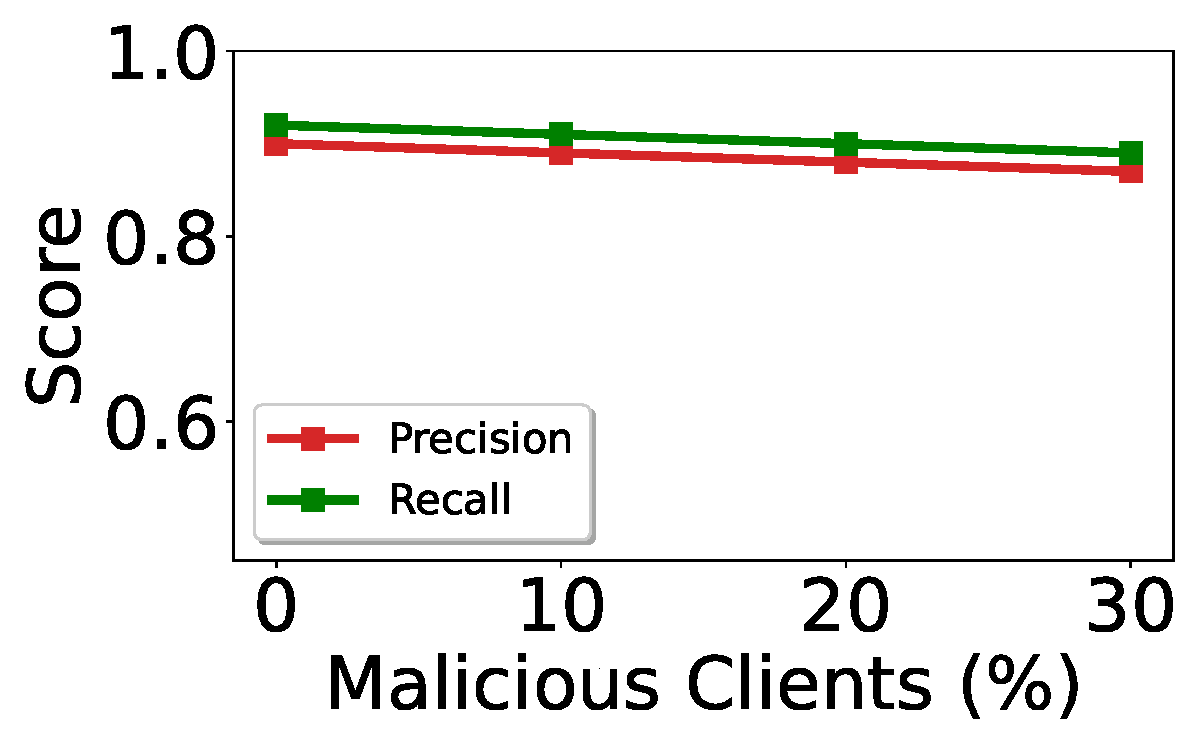
\includegraphics[height=0.15\textwidth]{fig/multi-krum.pdf}%
    \label{multikrumpoison}
  }
  \hfill
  \subfloat[Adversarial mimicry attack]{%
    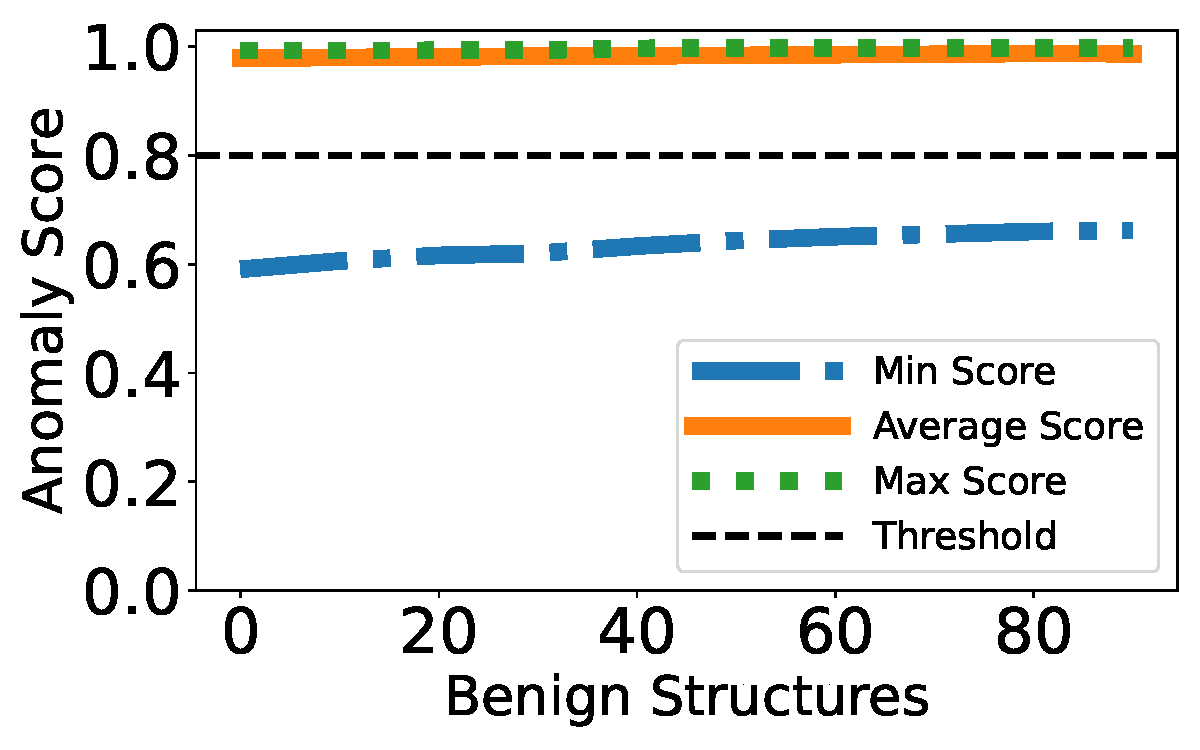
\includegraphics[height=0.15\textwidth]{fig/adversarial.pdf}%
    \label{mimicryattack}
  }
  \hfill
  \caption{Adversarial attacks analysis.}
  \label{fig:poison}
  \vspace{-3ex}
\end{figure*}

\PP{Mimicry Attacks}  We evaluated our system's resilience against the adversarial mimicry attack detailed by Goyal et al.~\cite{goyal2023sometimes} and compared its robustness with \flash. The attack aims to mimic benign graph embeddings, integrating benign node structures to evade detection. Using the E3 dataset, similar to \flash for fair comparison, our findings (shown in Figure~\ref{mimicryattack}) reveal that our detector remains robust; the integration of benign structures has a minimal impact on anomaly scores. Our system's superior robustness is due to our process-categorization-based ensemble \gnnshort architecture, which allows model specialization for different system entities, enhancing detection of structural changes. Conversely, \flash, relying on a generalized model for anomaly detection, exhibits vulnerabilities to mimicry attacks, as it may miss critical details. As demonstrated by the authors, \flash initially experiences a drop in anomaly scores, increasing the likelihood of attack nodes evading detection which is a vulnerability not present in our system. \footnote{PROVNINJA~\cite{mukherjee2023evading} is another mimicry attack that uses benign process profiles to find adversarial evasion strategies. It faces challenges against \pids like \flash and \Sys due to their multimodal architecture, which combines \wordvec for featurization and \gnnshort for anomaly detection. This complexity makes it difficult for attackers to create effective evasion strategies without accessing \wordvec directly or excessively querying the model, which conflicts with the black box nature of the assumed threat model of PROVNINJA.}


\PP{Model Poisoning Attacks} These occur when one or more malicious clients submit corrupted local model updates to the central server during training, thereby degrading the model’s performance. Existing methods typically assume an attack-free training phase, providing no defense against such attacks. We conducted experiments on the \optc dataset to assess the impact of poisoning attacks on our system, and we also evaluated how robust aggregation methods, such as Multi-Krum~\cite{munoz2019byzantine}, can enhance resilience.

Multi-Krum compares each client’s gradient with those of other clients, retaining only the most consistent updates. Since malicious updates must deviate significantly from benign ones to degrade performance, Multi-Krum effectively identifies and discards them as outliers. Figure~\ref{fig:poison} shows our experimental results using both FedAvg and Multi-Krum. With simple federated averaging, malicious noise critically affects the model by disrupting the benign distribution it learns. In contrast, Multi-Krum isolates and removes erroneous updates from malicious clients, preserving the global model. Notably, Multi-Krum assumes that fewer than one-third of all clients are malicious; therefore, in our experiments, we tested with a maximum of 30\% compromised clients.



\PP{Gradient-based Attacks} These attacks~\cite{chakraborty2021survey} exploit detailed knowledge of the target model, including its architecture and parameters, to calculate and apply malicious perturbations. Such white-box access allows an attacker to compute precise gradients that indicate how inputs should be modified to degrade the model’s performance. Other attacks tend to be black-box in nature, relying on iterative, query-based techniques to influence the model’s decisions. However, these repeated computations and queries run counter to the attacker’s aim of remaining inconspicuous, as they generate substantial activity and leave a significant footprint. Consequently, such attacks are often impractical in real-world scenarios. Several defenses can be employed during model training to bolster the system’s resilience against these threats. Adversarial training~\cite{tramer2019adversarial} is one effective strategy in which the model is trained on perturbed input data, thereby increasing its robustness against these attacks.

\PP{Bin-level Inference Attacks}  
In addition to the privacy risks outlined in Section~\ref{sec:privacy}, we identify another potential avenue for information leakage: bin-level inference attacks during training. In this scenario, a malicious client attempts to infer information about system entities held by other clients. It does so by manipulating the tokens it submits and observing changes in the utility server's harmonized vectors. Since overlapping token vectors are averaged, any noticeable change in the returned vector indicates that the token is shared across clients within the organization.  However, unlike the central and utility server inference risks, this attack does not compromise client identities and only the presence of a token in the system is revealed, preserving anonymity. Furthermore, our threat model~\ref{sec:threat}, consistent with prior \pids works, assumes a benign training environment free from adversarial clients. Bin-level inference attacks are thus only feasible during the training-time harmonization phase and not during deployment. We leave the development of federated learning methods robust to such adversarial training settings as an important direction for future work.


\PP{Alert Investigation} In systems like \Sys, validating the veracity of alerts is crucial for ensuring system reliability and preventing alert fatigue~\cite{nodoze2019}, traditionally involving security analysts manually reviewing each alert based on activities within local provenance graphs. This manual process, while thorough, is time-consuming and prone to errors, posing challenges in scalability and privacy. To enhance privacy and maintain efficiency in alert verification, implementing privacy-preserving techniques such as Secure Multi-party Computation (SMC)~\cite{goldreich1998secure}, Homomorphic Encryption (HE)~\cite{yi2014homomorphic}, and Zero-Knowledge Proofs (ZKP)~\cite{fiege1987zero} is vital. SMC allows multiple stakeholders to collaboratively validate alerts by jointly computing functions over their inputs while keeping those inputs private. HE enables the central server to analyze encrypted data, ensuring data confidentiality, and ZKP offers a way for one party to prove the validity of an alert to another without revealing any other information. Leveraging these technologies allows \Sys to privately and securely validate alerts, enhancing the system's trustworthiness and optimizing operational workflow. We identify privacy-preserving alert verification as a promising research direction. We leave it to future work to develop methods for privately sharing alert data with a central server, enabling security analysts to perform more in-depth attack analysis.

\PP{Explainability} The use of deep learning models in \pids makes them black-box systems, making it difficult to explain the inner decision-making process of these systems. Similar to existing \pids~\cite{flash2024,cheng2023kairos,yangprographer}, \Sys also suffers from this interpretability problem. This issue slows the adoption of these \pids compared to rule-based systems. Existing techniques~\cite{antwarg2021explaining,brown2018recurrent,ardito2021revisiting,hwang2021sfd} for model explainability focus on metrics such as feature importance. However, modern \pids use complex feature engineering techniques. For example, \flash uses a \wordvec model for feature generation from textual attributes in audit logs. These features are then used in a \gnn model for anomaly detection. The use of this multi-model approach renders existing explainable AI techniques impractical for these \pids. We identify explainable \pids as an important area for future research. The recent advancements in Large Language Models (LLMs)~\cite{chang2024survey} from the domain of Natural Language Processing can be utilized to solve this challenge. Future work can focus on using the reasoning power of LLMs to develop techniques for explaining \pids outputs.

\PP{Log Retention} Effective log retention \cite{wilbert2012log} is critical for the performance and reliability of \pids. Advanced Persistent Threats (APTs) can span months; therefore, logs need to be stored for extended periods to allow for thorough attack investigations. Decentralized systems like \Sys and \disdet \cite{dong2023distdet} keep raw logs on client machines. However, client machines have limited storage, so they can only store logs for a limited period. The duration for storing these logs depends on the domain in which \Sys is deployed. Secure and tamper-resistant cloud storage solutions \cite{kumar2018secure} can be combined with \Sys to securely back up user logs. In the event of an attack investigation, the logs corresponding to the alert raised by \Sys can be fetched from storage. These logs can then be processed to remove sensitive attributes to preserve user privacy \cite{portillo2019towards}. These logs can then be used for attack investigation.

\PP{Concept Drift} This is a problem where the data distribution of the underlying system evolves over time. For instance, with the emergence of new system activities, the patterns learned by \Sys during training might not remain valid. This drift could lead to misclassifications, as new benign behaviors might be mistakenly identified as anomalies. One mitigation strategy for this involves periodic retraining with more recent data to update the models. Techniques mentioned in recent works~\cite{lu2018learning, barbero2022transcending,jordaney2017transcend} can be leveraged to deal with the problem of concept drift.

\PP{State Explosion in Massive Networks} Scaling FL to larger enterprise networks introduces potential state explosion issues, primarily due to the increasing complexity in managing and integrating updates from a growing number of clients. As more clients participate, each contributing their local model updates, the volume of data to be processed and aggregated can increase significantly. This escalation can strain communication channels, leading to higher bandwidth requirements and increased latency. Furthermore, the aggregation process itself becomes more computationally demanding as the number of updates grows. \Sys addresses these challenges by utilizing an ensemble learning approach and categorizing system activities, which simplifies the aggregation by processing more uniform data segments. Moreover, our system uses models with small network overhead to prevent bandwidth challenges. To further enhance efficiency, additional techniques such as model compression~\cite{choudhary2020comprehensive}, selective update aggregation~\cite{ye2020federated} and the implementation of more robust communication protocols~\cite{laclau2020robust} can significantly improve handling large volumes of updates, thus preventing state explosion and maintaining system performance in large-scale federated learning environments.

% \wajih{add citations for different techniques (SMC, HE, etc.) below}

%\PP{Retraining Frequency} \wajih{Discuss here how often we need to retrain models on client machines. You can say that it depends on enterprise settings, in our experiments we found that XXX times per day gave us good results.}

%\wajih{Investigation using \Sys. We need to add one paragraph saying something about how to do an investigation using \Sys after detection. It does not have to be detailed. We just need to show that we thought about this problem. At the end of the paragraph say that we leave this for future work.}

%\wajih{Talk about why we did not consider other privacy-preserving techniques beyond the federation, such as secure multi-party computation or homomorphic encryption.}
\section{Conclusion}
\label{s:conclusion}
TODO

% \section{Ethics Considerations and Compliance with the Open Science Policy}
\label{sec:ethics}

In conducting our research, we strictly adhere to all ethical guidelines and the USENIX open science policy. Below are the key ethical considerations:

\begin{itemize}[leftmargin=*,itemsep=0.1em, parsep=0em, topsep=0em]
\item Our research does not identify any new vulnerabilities.
\item We conduct all experiments in a controlled environment using open-source datasets, ensuring no live systems are tested without informed consent.
\item Our activities do not violate any terms of service and involve no human subjects. 
\item Our research has not negatively impacted any team members and complies with all relevant laws. \item We are committed to transparency, making our research, systems, scripts, and datasets available to the public to enable reproduction and extension of our work. 
\end{itemize}

% \section{Acknowledgment}
\label{s:ack}


% \balance
% \bibliographystyle{plain}
% {
% \footnotesize
% \setlength{\bibsep}{3pt}
% \bibliography{bib-files/hassan,bib-files/hassan-misc}
% }
% % \section{Appendix}
% \label{sub:hyper}

% In  federated learning, where data originates from diverse sources such as user machines running various processes, quantifying this diversity becomes crucial for model development. The Shannon Diversity Index (SDI) is a metric adapted from ecology to measure the heterogeneity of datasets. This report elaborates on the application of SDI in federated learning, focusing on comparing the diversity of sub-models in an ensemble approach to a single model scheme.

% \section*{The Shannon Diversity Index (SDI)}

% SDI quantifies a dataset's diversity by considering both the variety of items (richness) and the distribution frequency of each item (evenness). It is given by:

% \[
% H' = -\sum_{i=1}^{R} p_i \ln(p_i)
% \]

% where:
% \begin{itemize}
%     \item $H'$ is the Shannon Diversity Index,
%     \item $R$ denotes the number of unique items,
%     \item $p_i$ represents the proportion of the dataset made up by the $i$th item.
% \end{itemize}

% In federated learning, SDI can reveal the heterogeneity within the data, guiding the strategy for model training and data segmentation.

% \section*{Application of SDI in Federated Learning}

% \subsection*{Scenario Overview}

% A federated learning setup involves analyzing process data from user machines. This scenario examines the diversity of processes, considering the significant overlap among users.

% \subsection*{Example Dataset}

% The dataset features processes like Chrome, Excel, Spotify, and others, from four user machines. Each machine's processes exhibit a 50\% overlap with others, presenting a realistic view of data distribution.

% \subsection*{Process Distribution Across Users}

% \begin{itemize}
%     \item \textbf{User 1}: \{Chrome, Excel, Spotify, Zoom, Slack\}
%     \item \textbf{User 2}: \{Word, PowerPoint, Teams, Slack, Spotify\}
%     \item \textbf{User 3}: \{Chrome, Zoom, Teams, Excel, Word\}
%     \item \textbf{User 4}: \{PowerPoint, Spotify, Slack, Chrome, Word\}
%     \item \textbf{User 5}: \{Chrome, Zoom, Teams\}

% \end{itemize}

% Processes are then randomly divided into three groups.

% \subsection*{Computing SDI for Each Group and single  Scheme}

% SDI calculations are based on the occurrence frequencies of processes, assessing diversity within each group and comparing it to a single  model approach where all processes are considered together.

% \subsubsection*{SDI Results}

% \begin{itemize}
%     \item \textbf{Category 1}: {Chrome, Zoom, and Teams}.
%     \item \textbf{Category 2}: {Word, Excel, and PowerPoint}.
%     \item \textbf{Category 3}: {Spotify and Slack}.
% \end{itemize}

% \subsection*{Analysis and Implications}

% \begin{itemize}
%     \item \textbf{Category 1 SDI}: $H' = 1.08$
%     \item \textbf{Category 2 SDI}: $H' = 1.10$
%     \item \textbf{Category 3 SDI}: $H' = 0.67$
%     \item The single  model, considering all processes together, yielded an SDI of $H' = 2.06$.
% \end{itemize}

% \subsubsection*{Diversity Comparison}

% Compared to the single  model's SDI, each sub-model reflects a specific aspect of the overall diversity but with reduced complexity, suggesting that sub-models focus on more homogeneous subsets of data.

% \subsubsection*{Influence on Client Fairness}

% By dividing the overall task into sub-tasks (sub-models) and assigning them to different subsets of processes (or data features), the influence of clients with large datasets is diversified across multiple models. This can prevent any single client from disproportionately skewing the outcome of the entire federated learning system.

% \subsubsection*{Balanced Representation}

% Each sub-model specializes in a different aspect of the data, potentially leading to a scenario where clients contribute more evenly across the ensemble. Clients with large datasets still contribute significantly, but their impact is more evenly distributed, enhancing fairness.



\balance
\bibliographystyle{IEEEtranS}
{
\footnotesize
\setlength{\bibsep}{3pt}
\bibliography{bib-files/hassan,bib-files/hassan-misc}}
% \section{Appendix}
% \label{sub:hyper}

% In  federated learning, where data originates from diverse sources such as user machines running various processes, quantifying this diversity becomes crucial for model development. The Shannon Diversity Index (SDI) is a metric adapted from ecology to measure the heterogeneity of datasets. This report elaborates on the application of SDI in federated learning, focusing on comparing the diversity of sub-models in an ensemble approach to a single model scheme.

% \section*{The Shannon Diversity Index (SDI)}

% SDI quantifies a dataset's diversity by considering both the variety of items (richness) and the distribution frequency of each item (evenness). It is given by:

% \[
% H' = -\sum_{i=1}^{R} p_i \ln(p_i)
% \]

% where:
% \begin{itemize}
%     \item $H'$ is the Shannon Diversity Index,
%     \item $R$ denotes the number of unique items,
%     \item $p_i$ represents the proportion of the dataset made up by the $i$th item.
% \end{itemize}

% In federated learning, SDI can reveal the heterogeneity within the data, guiding the strategy for model training and data segmentation.

% \section*{Application of SDI in Federated Learning}

% \subsection*{Scenario Overview}

% A federated learning setup involves analyzing process data from user machines. This scenario examines the diversity of processes, considering the significant overlap among users.

% \subsection*{Example Dataset}

% The dataset features processes like Chrome, Excel, Spotify, and others, from four user machines. Each machine's processes exhibit a 50\% overlap with others, presenting a realistic view of data distribution.

% \subsection*{Process Distribution Across Users}

% \begin{itemize}
%     \item \textbf{User 1}: \{Chrome, Excel, Spotify, Zoom, Slack\}
%     \item \textbf{User 2}: \{Word, PowerPoint, Teams, Slack, Spotify\}
%     \item \textbf{User 3}: \{Chrome, Zoom, Teams, Excel, Word\}
%     \item \textbf{User 4}: \{PowerPoint, Spotify, Slack, Chrome, Word\}
%     \item \textbf{User 5}: \{Chrome, Zoom, Teams\}

% \end{itemize}

% Processes are then randomly divided into three groups.

% \subsection*{Computing SDI for Each Group and single  Scheme}

% SDI calculations are based on the occurrence frequencies of processes, assessing diversity within each group and comparing it to a single  model approach where all processes are considered together.

% \subsubsection*{SDI Results}

% \begin{itemize}
%     \item \textbf{Category 1}: {Chrome, Zoom, and Teams}.
%     \item \textbf{Category 2}: {Word, Excel, and PowerPoint}.
%     \item \textbf{Category 3}: {Spotify and Slack}.
% \end{itemize}

% \subsection*{Analysis and Implications}

% \begin{itemize}
%     \item \textbf{Category 1 SDI}: $H' = 1.08$
%     \item \textbf{Category 2 SDI}: $H' = 1.10$
%     \item \textbf{Category 3 SDI}: $H' = 0.67$
%     \item The single  model, considering all processes together, yielded an SDI of $H' = 2.06$.
% \end{itemize}

% \subsubsection*{Diversity Comparison}

% Compared to the single  model's SDI, each sub-model reflects a specific aspect of the overall diversity but with reduced complexity, suggesting that sub-models focus on more homogeneous subsets of data.

% \subsubsection*{Influence on Client Fairness}

% By dividing the overall task into sub-tasks (sub-models) and assigning them to different subsets of processes (or data features), the influence of clients with large datasets is diversified across multiple models. This can prevent any single client from disproportionately skewing the outcome of the entire federated learning system.

% \subsubsection*{Balanced Representation}

% Each sub-model specializes in a different aspect of the data, potentially leading to a scenario where clients contribute more evenly across the ensemble. Clients with large datasets still contribute significantly, but their impact is more evenly distributed, enhancing fairness.


\end{document}